\documentclass[11pt]{report}

% ---------- Packages ----------
\usepackage[utf8]{inputenc}
\usepackage[T1]{fontenc}
\usepackage{amsmath,amssymb,amsthm}
\usepackage{grffile}
\usepackage{graphicx}
\usepackage{booktabs}
\usepackage{array}
\usepackage{siunitx}
\usepackage{listings}
\usepackage{xcolor}
\usepackage{hyperref}
\usepackage{cleveref}
\usepackage{geometry}
\usepackage{fancyhdr}
\usepackage{caption}
\usepackage{subcaption}
\usepackage{bm}
\usepackage[round,authoryear]{natbib}

\geometry{margin=1in}

% ---------- Hyperref setup ----------
\hypersetup{
    colorlinks=true,
    linkcolor=blue!60!black,
    citecolor=green!50!black,
    urlcolor=magenta,
    pdftitle={DRAGON: Documentation},
    pdfauthor={Bobbie},
}

% ---------- Header/Footer ----------
\pagestyle{fancy}
\fancyhf{}
\fancyhead[L]{DRAGON LORE}
\fancyhead[R]{\leftmark}
\fancyfoot[C]{\thepage}

% ---------- Code listing style ----------
\lstdefinestyle{codestyle}{
    backgroundcolor=\color{gray!10},
    commentstyle=\color{green!50!black},
    keywordstyle=\color{blue},
    numberstyle=\tiny\color{gray},
    stringstyle=\color{orange},
    basicstyle=\ttfamily\footnotesize,
    breakatwhitespace=false,
    breaklines=true,
    captionpos=b,
    keepspaces=true,
    numbers=left,
    numbersep=5pt,
    showspaces=false,
    showstringspaces=false,
    showtabs=false,
    tabsize=2,
    frame=single,
}
\lstset{style=codestyle}

% ---------- Custom math commands ----------
\renewcommand{\d}[1][ ]{\ensuremath{\operatorname{d}\!{#1}}}
\newcommand{\pd}[2]{\frac{\partial #1}{\partial #2}}

\newcommand{\cpp}[1]{\lstinline[language=C++]{#1}}
\newcommand{\bash}[1]{\lstinline[language=bash]{#1}}
\newcommand{\py}[1]{\lstinline[language=Python]{#1}}

% ---------- Title page info ----------
\title{\textbf{DRAGON}\\ Divergence-Regulation for Adaptive Godunov-Oriented Numerics\\ Literary Overview \& Reference Entries (LORE) Document}
\author{Bobbie Markwick}
\date{19 August 2026}

\begin{document}

% ================= Title Page =================
\pagenumbering{roman}
\maketitle

%\begin{abstract}\end{abstract}

\tableofcontents

\clearpage
\pagenumbering{arabic}
\setcounter{page}{1}

% ================= Introduction =================
%\chapter{Introduction} \label{ch:intro}

%\section{Motivation and Scope}
% TODO: Describe the scientific motivation for DRAGON, the physical  regimes it targets, and the problems it is designed to solve.

%\section{Overview of Capabilities}
% TODO: Summarize physics modules, dimensionality, geometries,  boundary conditions, and any special features (e.g., AMR, GPU support).

%\section{Document Organization}
%This document is organized as follows....



% ================= Code Structure =================
\chapter{Code Structure}
\label{ch:code}

\section{Directory Layout}
\begin{lstlisting}[language=bash, caption={Repository layout}]
DRAGON/                    # repository root
|-- DRAGON/                # core solver source
|   |-- Boundary/          # boundary conditions
|   |-- FluidElement/      # primitive/conservative state & arithmetic
|   |-- Hydro/             # hydrodynamic solver
|   |   |-- CFL/           # timestep control
|   |   |-- ExtendedArray/ # multidimensional arrays with ghost cells
|   |   |-- Godunov/       # split/unsplit driver, flux application
|   |   |-- Reconstruction/# MUSCL interface-state reconstruction
|   |   |-- Riemann/       # Exact, HLL, HLLE, HLLC, HLLD, Roe solvers
|   |-- MHD/               # constrained transport (E-field, Faraday, body fields)
|   |-- Passives/          # passive scalars 
|   |-- Refinement/        # domain decomposition (DistGrid)
|   |-- main/              # program entry point & problem setup
|   |-- Config.h, Constants.h, Problem.cpp
|-- DRAGONWING/            # memory management & multithreading
|   |-- Atomics/           # atomic counters
|   |-- Memory/            # RAII scratch arrrays
|   |-- Multithreading/    # multithreading
|-- DRAGONHOARD/           # HDF5 output & restart I/O
|-- DRAGONGAZE/            # Python visualisation/analysis scripts
|-- DRAGONLORE/            # this documentation
|-- Examples/              # example problem setups
|   |-- 1D/                # shock tubes
|   |-- Hydro/             # 2D and 3D Hydro examples
|   |   |-- Blast/, Diagonal/, Kelvin-Helmholtz/
|   |-- MHD/               # 2D and 3D MHD examples
|   |   |-- Blast/, LoopAdvection/, MHDRotor/, Orszag-Tang/, Waves/
|-- Testing/               # unit tests
|   |-- Core/
|-- LICENSE                #Apache License
|-- README.md
\end{lstlisting}

\section{Data Structures}
\label{sec:data-structures}

\subsection{Fluid Elements}
\label{sec:fluid-elements}

The following data types are defined in \bash{DRAGON/FluidElement/FluidElement.h}

\subsubsection{vec3}

\cpp{DRAGON::vec3} is a plain structure with $x,y,z$ components.
The following operations are supported:
\begin{itemize}
\item Addition (\cpp{+}, \cpp{+=}) and Subtraction  (\cpp{-}, \cpp{-=}) with another \cpp{vec3}.
\item Multiplication (\cpp{*}, \cpp{*=}) and Division  (\cpp{/}, \cpp{/=}) by a scalar \cpp{double}.
\item Dot (\cpp{*}) and cross (\cpp{cross(v1, v2)}) product between two \cpp{vec3}'s.
\item Swapping two components, either in place (e.g. \cpp{swapXY()}) or on a copy (e.g. \cpp{swappedXY()}).
\end{itemize}

\subsubsection{PrimitiveState}

\cpp{DRAGON::PrimitiveState} represents a single fluid element (i.e.\ one cell's state), which contains density \cpp{rho}, pressure \cpp{p}, velocity vector \cpp{v}, and (MHD only) magnetic field vector \cpp{B}. This is the form the solver reconstructs, applies boundary conditions to, and reports as output.

As already noted in \Cref{ch:physics}, \cpp{B} is stored in Gaussian (non-rationalized) units, so the code is explicit about factors of $4\pi$ wherever they appear -- concretely, \bash{Constants.h} predefines \cpp{_1_4pi} ($=1/4\pi$), \cpp{_1_8pi} ($=1/8\pi$), and \cpp{sq4pi} ($=\sqrt{4\pi}$) rather than dividing by $4\pi$ inline. %and both energy density and pressure conversions add/remove a magnetic term $\mathbf{B}^2/8\pi$.

\subsubsection{ConservativeState}

\cpp{DRAGON::ConservativeState} represents a fluid element in conservative form: mass density \cpp{rho}, energy density \cpp{E}, momentum density vector \cpp{mom}, and (MHD only) \cpp{B}. This is the form fluxes are computed and applied in: rather than a true fluid element, a particular instance of \cpp{ConservativeState} might instead represent a flux (times one computational unit time per computational unit length).

The following fluid arithmetic operations are supported by \cpp{ConservativeState}
\begin{itemize}
\item Addition (\cpp{+}, \cpp{+=}) and Subtraction  (\cpp{-}, \cpp{-=}) with another \cpp{ConservativeState}.
\item Multiplication (\cpp{*}, \cpp{*=}) and Division  (\cpp{/}, \cpp{/=}) of all components by a \cpp{double}.
\item Swapping two dimensions as with \cpp{vec3}. This swaps the corresponding components of both \cpp{mom} and \cpp{B}. \cpp{PrimitiveState} also supports this operation directly (using \cpp{v} instead of \cpp{mom}).
\end{itemize}

Both \cpp{PrimitiveState} and \cpp{ConservativeState} are constructible from the other (\cpp{ConservativeState(PrimitiveState)} and \cpp{PrimitiveState(ConservativeState)}).  This can be done explicitly via the other, and is also done implicitly whenever a \cpp{PrimitiveState} is used in fluid arithmetic. 
If you need to directly add or subtract the components of two \cpp{PrimitiveState}'s, you will need to do this manually on each component.

Both types also provide a number of other physically relevant quantities, such as various wave speeds, \cpp{energy()} or \cpp{pressure()} on a primitive or conservative state, and \cpp{flux()} to calculate the fluxes of the governing MHD equations (\ref{eq:MHD}). The \cpp{flux()} function returns the flux in the $x$-direction, and in MHD includes the electric fields from the induction equation as the \cpp{B} components (see \Cref{sec:ct}).  When called from a \cpp{ConservativeState}, \cpp{flux()} can optionally take the velocity \cpp{v} if already known; otherwise \cpp{v} is computed from \cpp{mom} and \cpp{rho}.


\subsection{ExtendedArray}
\label{sec:extendedarray}
Grid storage is built on a small family of templates in \bash{DRAGON/Hydro/ExtendedArray}: \cpp{ExtendedArray1D<T>}, \cpp{ExtendedArray2D<T>}, and \cpp{ExtendedArray3D<T>}. Each owns a single flat, row-major heap array sized to include a configurable ghost margin.
Accessing elements within an extended array is done via \cpp{array[i]}, \cpp{array[i,j]}, or \cpp{array[i,j,k]} depending on the array's dimension\footnote{It is for this reason that DRAGON requires C++23}. 
\cpp{i}, \cpp{j}, or \cpp{k} may be negative or exceed that dimension's size by an amount up to the array's ghost margin; in this case the accessed quantity corresponds not to a physical item but to cell within the boundary layer\footnote{Or, in the case of domain decomposition (\Cref{sec:distgrid}), it might be a cell owned by another subgrid.}.
When DRAGON is built for testing, every cell access will assert that the bounds of the ghosts are within the valid range; this check is compiled out in production builds.

\cpp{ExtendedArray} objects can't be copied using normal C++ syntax, but the contents of one array can be copied to another (with identical dimension) using  \cpp{clone(ref, copyghosts)}. Ghost cells are copied only if \cpp{copyghosts} is true.

\bash{ArrayTypes.hpp} defines the concrete array types used throughout the solver as typedefs over these templates and \cpp{PrimitiveState}/\cpp{ConservativeState}/\cpp{vec3} (\Cref{sec:fluid-elements}) -- e.g.\ \cpp{FluidArray2D = ExtendedArray2D<PrimitiveState>}, \cpp{FluxArray3D = ExtendedArray3D<ConservativeState>}, \cpp{MagneticArray2D = ExtendedArray2D<vec3>}. 


\subsection{Grid}
\label{sec:grid}

Fundamentally, a \cpp{DRAGON::Grid} (\bash{DRAGON/Hydro/Grid.hpp}) is one or more extended arrays together with a boundary condition and the ability to advance the arrays in time. 

The abstract \cpp{Grid} base class declares the two pure-virtual per-step advancement functions \cpp{split_step(dt)}/\cpp{unsplit_step(dt)}, the CFL-aware driver \cpp{advance(dt, check_cfl)} which wraps either \cpp{advance_split}/\cpp{advance_unsplit} (\Cref{sec:CFL}), and the virtual failure hook \cpp{on_step_fail(e)} used by the retry-with-halving loop.

The dimension-specific subclasses \cpp{Grid1D}/\cpp{Grid2D}/\cpp{Grid3D} each own one \cpp{FluidArray1D/2D/3D w} (\Cref{sec:extendedarray}) as their primary state, plus a staggered \cpp{MagneticArray2D/3D B} in MHD builds (\Cref{sec:ct}).
The magnetic field is stored on a staggered face-centred grid, with \cpp{B[i,j,k].x} corresponding to $B_{i-\frac12,j,k}^x$, \cpp{B[i,j,k].y}  to $B_{i,j-\frac12,k}^y$, and \cpp{B[i,j,k].z}  to $B_{i,j,k-\frac12}^z$.
 External functions can access a reference to the staggered magnetic array via \cpp{grid._B()}.


\section{Dependencies}
\label{sec:dependencies}

DRAGON's only dependency is \textbf{HDF5} \citep{HDFGroup}, used by DRAGONHOARD (\Cref{ch:hoard})\footnote{Core DRAGON and DRAGONWING are agnostic to the file storage format, so if HDF5 is for some reason unavailable on your system, you would only need to modify DRAGONHOARD to interface with your alternative format.} for output and restart I/O.
No other third-party library is required to build or run DRAGON itself.

DRAGON's in-house visualisation toolkit DRAGONGAZE (\Cref{ch:gaze}) depends separately on \textbf{h5py} (to read the HDF5 files DRAGONHOARD writes) and \textbf{Matplotlib} (to render plots from that data). These are Python-side dependencies only and do not affect the C++ build.


On macOS, HDF5 can be installed with Homebrew:
\begin{lstlisting}[language=bash]
brew install hdf5
brew --prefix hdf5
\end{lstlisting}
The second command prints the path to the HDF5 installation on your computer. This will usually \bash{/opt/homebrew/opt/hdf5} on Apple Silicon Macs, or \bash{/usr/local/opt/hdf5} on Intel Macs.



On Linux, install HDF5 through your system package manager -- for example, on Debian/Ubuntu:
\begin{lstlisting}[language=bash]
sudo apt install libhdf5-dev
\end{lstlisting}


\section{Style Guide}

This section contains a style guide for developers who wish to contribute to DRAGON.

\subsection{File Headers}

Every file opens with a comment block:
\begin{lstlisting}[language=C++]
//
//  <Filename>
//  <DirectoryPath>
//
//  Created by <original developer> on <creation date>.
//  <citations, if applicable>
//
\end{lstlisting}
Here \bash{<Filename>} is the name of the file (including extension), and \bash{<DirectoryPath>} is relative to the project root.

Each in-code citation should include author names, year, and a link. arXiv links  are preferred if available, as this makes the papers available to users who don't belong to an institution. For sources not on arXiv, use a doi link if possible. 
If you implemented something based on the description in source A's description of a method first published in source B, you should cite as follows:
\begin{lstlisting}[language=C++]
//  Implemented based in part on <citation for source A>
//      <citation(s) for source(s) B>
\end{lstlisting}
In addition to comment citations, also give a full citation in the bibliography of this document.

\subsection{Header guards}
The traditional pattern is preferred. Typically, the you should name it after the file stem.
\begin{lstlisting}[language=C++]
#ifndef Grid_hpp
#define Grid_hpp
...
#endif
\end{lstlisting}

\subsection{Includes}

Includes should be grouped in the following order, leaving a blank line between each group
\begin{enumerate}
\item Header files defining things that this file implements
\item  Includes which are used in a major way.
\item Includes which are used in a minor way.
\item Includes which are only used in error paths.
\end{enumerate}
For header files other than in the first group, you should also include a trailing comment saying \textit{why} this header is included. Trailing comments in the same group should have their starting points vertically aligned. Comments may be omitted if the file is being used for a data type which shares its name with the include, and for the module's configuration header.

For example, the includes in \bash{CFL.cpp} are
\begin{lstlisting}[language=C++]
#include "CFL.hpp"

#include "Config.h"
#include <cmath>        //For std::abs, sqrt, pow
#include <algorithm>    //For std::min/max

#include "Boundary/GhostFill.hpp"   //For boundary.apply

#include <stdexcept>    //For std::runtime_error (CFL timestep fails to compute)
#include <exception>    //For handling step restarts
#include <iostream>     //For printing step-restart messages
#include <cstdlib>      //For exit() if the timestep gets too small
\end{lstlisting}
This file implements everything declared in \bash{CFL.hpp}.
\bash{Config.h} defines which of this file's calculation methods should be active, and the various \cpp{std::} functions are used heavily throughout the implmentation, so these includes qualify as major usage. \cpp{boundary.apply} meanwhile is only called in a couple of places, so it is considered a minor item. Lastly, the last four includes are only used to handle step restarts, so they are considered error-path-only.


Immediately after the includes, source files typically contain \cpp{using namespace DRAGON;} (and/or any other namespace they live in).
Each of the top-level modules has its own namespace of the same name: \cpp{DRAGON}, \cpp{DRAGONWING}, \cpp{DRAGONHOARD}. 
Sub-areas get nested namespaces rather than longer names: \cpp{DRAGON::CONFIG}, \cpp{DRAGON::Boundary}, etc. 

\subsection{Naming}

\paragraph{Types}are PascalCase: \cpp{PrimitiveSate}, \cpp{Grid1D}, \cpp{ArrayGuard}. As an exception, \cpp{vec3} is lowercase. Namespaces are also PascalCase, except for top-level modules since those are acronyms.

\paragraph{Functions}are typically either camelCase (e.g. \cpp{swapXY}, \cpp{getSize}, \cpp{waitForCompletion}) or snake\_case (e.g. \cpp{advance_split}, \cpp{cfl_time}, \cpp{verify_and_fallback}). Named algorithms should however defer to the capitalisation seen in the literature (e.g. \cpp{HLL}, \cpp{Roe}, \cpp{MUSCL}, \cpp{CTU}).

\paragraph{Local variables} should stay short, and where possible should match symbols used in the physics (e.g. \cpp{rho}, \cpp{B}, \cpp{dx}, \cpp{nx}). 
However, variable names should avoid conflicting with other variable names if this could lead to confusion (e.g. momentum is \cpp{mom}, since \cpp{p} already refers to pressure). 
Loop indices should generally be \cpp{i}, \cpp{j}, \cpp{k} for $x$, $y$, and $z$ dimensions, plus \cpp{g} for ghost indices.


\paragraph{Compile-time options} in \bash{Config.h} (and corresponding files in other modules) should be SCREAMING\_SNAKE\_CASE (e.g. \cpp{RIEMANN_HLLX}, \cpp{CT_CONSV_TOTAL_E}) for preprocessor options and snake\_case (e.g. \cpp{timestep_tolerance}, \cpp{ct_energy_beta}).

\paragraph{Derived Constants}in \bash{Constants.h} use the format \cpp{_A_B} to refer to the fraction A/B. For example, \cpp{_1_4pi}$=\frac1{4\pi}$, or \cpp{_Gm1_2G}$= \frac{\gamma-1}{2\gamma}$.  Nonfractional constants may also include an underscore to avoid naming conflicts, such as \cpp{_gamma}. 



\subsection{Indentation}

Indent using four-space tabs\footnote{Here in the Cult of the DRAGON, we are \href{https://github.com/torvalds/linux/blob/master/Documentation/process/coding-style.rst}{heretics}.}. This is partly because I am used to Xcode's default, and partly because the ``You're nesting too much" crowd isn't usually nesting three dimensions of loops. 

\

\noindent \bash{Config.h} uses a specialindentation to encode which options belong to which setting:
\begin{itemize}
\item A \cpp{#define} indented and sitting \textit{above} another \cpp{#define}  is one of the enumerated choices for that setting (e.g. \cpp{RIEMANN_HLLC} is a choice for \cpp{RIEMANN_DEFAULT}).

\item A \cpp{#define} or \cpp{const} indented and sitting \textit{below} another \cpp{#define} is a parameter specific to that setting (e.g. \cpp{exact_riemann_max_iters} only matters when \cpp{RIEMANN_EXACT} is selected).

\end{itemize}
This is spelled out in further detail in a comment at the top of the file.

Outside of \bash{Config.h}, one should generally follow standard C++ indentation practices, with the following additional prescriptions:
\begin{enumerate}
\item Lines which purely serve an auxiliary purpose (e.g. calling \cpp{DRAGONWING} to allocate or release scratch memory) should be indented one extra line to keep the primary algorithm easier to read.
\item \cpp{#if}/\cpp{#ifdef} blocks should be at the same indentation level as both the surrounding and enclosed code. As such nested \cpp{#if}'s should generally be on the same indentation level.%, though an exception can be made if not doing so significantly hinders readability.
\item \cpp{case} statements should be at the \textit{same} indentation level as the \cpp{switch}. If a particular case requires multiple lines, indent after the first. 
\end{enumerate}

\subsection{Braces}
Opening braces should stay on the same line as the function signature or control statement.
Closing braces should be on their own line, except that \cpp{else} or \cpp{while} should be a single space come after the closing brace of an \cpp{if} or \cpp{do} statement (respectively, and when applicable).

For \cpp{if}-\cpp{else} statements, either all should use braces or none should. 
Except to compliance with the preceding guideline,  \cpp{if} statements with a single statement do not need braces, even if the statement is placed on its own line. 

\subsection{Spaces}

Spaces should be included after the following keywords
\begin{lstlisting}[language=C++]
if else switch case do while for
\end{lstlisting}
With most of these keywords you should also include a space before the opening brace. For functions however, there should be no space between the closing parentheses and the opening brace, unless there is some other keyword (e.g. \cpp{const}) between them, in which case that keyword should have a space on both sides.


Generally you should use spaces on each side any of the following operators:
\begin{lstlisting}[language=C++]
=  +  -  <  >  *  /  %  |  &  ^  <=  >=  ==  !=  ?  :
\end{lstlisting}
However, sometimes omitting some of these spaces can make larger mathematical statements easier to read by conveying order of operations. If this is the case, do that. For loops are another place where omitting these extra spaces is generally acceptable.

%\subsection{Miscellaneous}
%Pay no attention to style guides that recommend keeping your lines under a certain length, unless you want to.

% ================= Physical Model =================
\chapter{Physical Model \& Numerical Methods}
\label{ch:physics}

\section{Governing Equations}
The ideal MHD equations solved by DRAGON are, in conservative form:
\begin{subequations} \label{eq:MHD}
\begin{equation} \pd{\rho}{t} + \nabla\cdot (\rho \mathbf{v}) = 0 \end{equation} \label{eq:continuity} 
\begin{equation} \pd{}{t}\left(\rho \mathbf{v}\right) + \nabla\cdot \left[ \rho \mathbf{v}\mathbf{v} - \frac{1}{4\pi}\mathbf{B}\mathbf{B}  + \left(p + \frac{\mathbf{B}^2}{8\pi}\right)\mathbb{I} \right]= 0 \end{equation} \label{eq:momentum} 
\begin{equation} \pd{E}{t} + \nabla\cdot \left[ \left(E + p + \frac{\mathbf{B}^2}{8\pi}\right)\mathbf{v}    -  (\mathbf{v} \cdot \mathbf{B}) \mathbf{B} \right]= 0 \end{equation} \label{eq:energy} 
\begin{equation} \pd{\mathbf{B}}{t}  =  \nabla\times (\mathbf{v} \times \mathbf{B}) \end{equation} \label{eq:induction} 
subject to the constraint
\begin{equation} \nabla\cdot \mathbf{B} = 0. \label{eq:divb}\end{equation}
\end{subequations}
Here $\rho$ is mass density, $\mathbf{v}$ the fluid velocity, $\mathbf{B}$ the magnetic field, and $p$ the thermal pressure. 
$E$ the total energy density
\begin{equation} E = \frac{p}{\gamma - 1} + \frac{1}{2}\rho \mathbf{v}^2 + \frac{\mathbf{B}^2}{8\pi}, \end{equation}
where $\gamma$ adiabatic index.
DRAGON adopts Gaussian (non-rationalized) electromagnetic units, so the magnetic pressure and Lorentz force terms carry an explicit factor of $4\pi$. 

\section{Initial Conditions} \label{sec:initial}
In DRAGON, problem initialisation consists of three steps:
\begin{enumerate}
\item Hydrodynamic Initialisation
\item Magnetic Field Initialization
\item (Optional) Custom Additional Initialisation
\end{enumerate}

In the first step, the user implements \cpp{Problem::initialFluidState(x,y,z)} which returns a primitive hydrodynamic state $w = (\rho, \mathbf{v}, p)$ at position $(x,y,z)$.  The cell $w_{i,j,k}$ will be initialised with the state computed by this function with input position $( (i+\frac12)\d x, (j+\frac12)\d y, (k+\frac12)\d z)$. Any value of $\mathbf{B}$ provided in this step will be overridden in the following step, though there are cases where it is useful to compute a preliminary value of $\mathbf{B}$ at this stage.

In the second step, the user implements \cpp{Problem::initialMagneticPotential(x,y,z)} which returns vector potential $\mathbf A$ at position $(x,y,z)$. From this function, $\mathbf{B} = \nabla\times\mathbf{A}$ is initialised as follows:
\begin{enumerate}
\item $\mathbf A$ is calculated at every edge on the grid.
\begin{subequations}
\begin{equation} A^x_{i, j-\frac12, k-\frac12} = \mathbf{A}\left[\left(i+\frac12\right)\d x,j\d y, k\d z\right]_x\end{equation}
\begin{equation} A^y_{i-\frac12, j, k-\frac12} = \mathbf{A}\left[i\d x,\left(j+\frac12\right)\d y, k\d z\right]_y\end{equation}
\begin{equation} A^z_{i-\frac12, j-\frac12, k} = \mathbf{A}\left[i\d x,j\d y, \left(k+\frac12\right)\d z\right]_z\end{equation}
\end{subequations}
\item The normal component of $\mathbf{B}$ is calculated on each of the faces 
\begin{subequations}
\begin{equation} B^x_{i-\frac12, j,k} = \frac14\left(A^y_{i-\frac12, j,k-\frac12} + A^z_{i-\frac12, j+\frac12,k} - A^y_{i-\frac12, j,k+\frac12}  - A^z_{i-\frac12, j-\frac12,k}\right) \end{equation}
\begin{equation} B^y_{i, j-\frac12,k} = \frac14\left(A^z_{i-\frac12, j-\frac12,k} + A^x_{i, j-\frac12,k+\frac12} - A^z_{i+\frac12, j-\frac12,k}  - A^x_{i, j-\frac12,k-\frac12}\right)\end{equation}
\begin{equation} B^z_{i, j,k-\frac12}= \frac14\left(A^x_{i, j-\frac12,k-\frac12} + A^y_{i+\frac12, j,k-\frac12} - A^x_{i, j+\frac12,k-\frac12}  - A^y_{i-\frac12, j,k-\frac12}\right)\end{equation}
\end{subequations}
\item $\mathbf{B}_{i,j,k}$ is calculated as an average of the adjacent faces
\begin{subequations}
\begin{equation} B^x_{i, j,k} = \frac12\left(B^x_{i-\frac12,j,k} + B^x_{i+\frac12,j,k}\right)\end{equation}
\begin{equation} B^y_{i, j,k} = \frac12\left(B^y_{i,j-\frac12,k} + B^y_{i,j+\frac12,k}\right)\end{equation}
\begin{equation} B^z_{i, j,k} = \frac12\left(B^z_{i,j,k-\frac12} + B^z_{i,j,k+\frac12}\right)\end{equation}
\end{subequations}
\end{enumerate}
This procedure ensures that $\mathbf{B}$ is initialised with zero divergence everywhere.

In the final step, the user implements \cpp{Problem::completeProblemInit(grid)} to perform any additional initialisation steps on \cpp{grid}.

\section{Boundary Conditions} \label{sec:boundary}
DRAGON supports several types of boundary conditions, and provides capability for defining customisable boundary conditions.
All boundary conditions are subclasses of the \cpp{GhostFill} subclass, which are responsible for filling in the ghost cells on a \cpp{Grid} object. 
To set the boundary conditions for a problem, set the \cpp{boundary} property of the \cpp{Grid} class, for example
\begin{lstlisting}[language=C++]
grid.boundary = Periodic();
\end{lstlisting}
Every time the grid advances, it will call the \cpp{apply(Grid&)} function on its boundary object.

A boundary object can be restricted to specific faces by passing a string argument to the constructor. In this string, specify any combination of X, Y, Z, optionally adding plus or minus after any or all of these to only include the respective side\footnote{Plus and minus restriction is not supported for periodic boundary conditions}. For example, \cpp{Reflective("XZ-")} uses reflective boundary conditions on the $X_-$, $X_+$, and $Z_-$ boundaries.  Any faces not explicitly specified will default to outflow. 

Boundary conditions can be combined using the \cpp{+} operator. For example:
\begin{lstlisting}[language=C++]
grid.boundary = Reflective("XZ-") + Periodic("Y");
\end{lstlisting}
defines a box which is reflective in the $X_\pm$ and $Z_-$  boundaries, periodic in the $Y$ direction,  and defaults to outflow on the $Z_+$ boundary. Boundaries are applied in the order they are specified, with any implicit outflow being applied first. In the example, the reflective boundaries are applied before the periodic boundaries.

In addition to passing a face-restriction string, the GhostFill constructor also takes a boolean \cpp{corner_ghosts}. This value is true by default, and you should normally leave it that way. If \cpp{corner_ghosts} is true, then all ghosts on the corresponding side of the boundary will be filled. If it is false, then only the ghosts which are out of bounds in a single dimension are filled, and ghosts in the corner regions are assumed to have already been properly filled by a previous boundary object.

DRAGON includes the following built in boundary classes 

\subsection{Outflow}
The \cpp{Boundary::Outflow} class implements outflow (Neumann) boundary conditions, filing each ghost with the state of the nearest physical cell. Outflow boundaries are the default boundary if none is set.
Negative-side and positive-side ghosts  on an X boundary are filled as 
\begin{equation}
\begin{pmatrix}
\rho_{(-g,j,k)}\\
\mathbf{v}_{(-g,j,k)}\\
p_{(-g,j,k)}\\
B^y_{(-g,j,k)}\\
B^z_{(-g,j,k)}
\end{pmatrix} = \begin{pmatrix}
\rho_{(0,j,k)}\\
\mathbf{v}_{(0,j,k)}\\
p_{(0,j,k)}\\
B^y_{(g-1,j,k)}\\
B^z_{(g-1,j,k)}
\end{pmatrix}
,\qquad
\begin{pmatrix}
\rho_{(n_x-1+g,j,k)}\\
\mathbf{v}_{(n_x-1+g,j,k)}\\
p_{(n_x-1+g,j,k)}\\
B^y_{(n_x-1+g,j,k)}\\
B^z_{(n_x-1+g,j,k)}
\end{pmatrix} = \begin{pmatrix}
\rho_{(n_x-1,j,k)}\\
\mathbf{v}_{(n_x-1,j,k)}\\
p_{(n_x-1,j,k)}\\
B^y_{(n_x-1,j,k)}\\
B^z_{(n_x-1,j,k)}
\end{pmatrix}
\end{equation}
Normal magnetic fields however are linearly extrapolated to preserve $\nabla\cdot\mathbf{B} = 0$:
\begin{subequations}
\begin{equation} B^x_{(-g,j,k)} = 2B^x_{(-g+1,j,k)} - B^x_{(-g+2,j,k)}\end{equation}
\begin{equation} B^x_{(n_x+g,j,k)} = 2B^x_{(n_x-1+g,j,k)} - B^x_{(n_x-2+g,j,k)}\end{equation}
\end{subequations}

Calling \cpp{Boundary::Outflow::Gated} instead of the outflow constructor will return a modified outflow condition designed to inhibit accidental inflow. This variant follows all outflow criteria as normal, except that if the normal velocity is directed inwards to the physical region ($v_x >0$ on an $X_-$ boundary, $v_x<0$ on an $X_+$ boundary), that component will be set to zero in the boundary region. 

\subsection{Periodic}
The \cpp{Boundary::Periodic} class implements periodic boundary conditions, filling ghosts such that the ghost cells near the positive boundary match the physical cells near the corresponding negative boundary.
Negative-side ghosts are filled as $w_{-g,j,k} = w_{n_x-g,j,k}$ and positive-side ghosts are filled as $w_{n_x+g,j,k} = w_{g,j,k}$.
Face-magnetic ghosts are filled likewise for half-integer values of $g$. 

Note that periodic boundary conditions require that both the plus and minus boundaries of any given dimension are used; if restriction such as \cpp{Periodic("X-")} is attempted, the object will initialise such that sides will be used (in this case, equivalent to \cpp{Periodic("X")}).

\subsection{Reflective}
The \cpp{Boundary::Reflective} class implements reflective boundary conditions, filling ghosts such that they mirror the nearby physical cells. These conditions mimic a stationary wall, which in MHD is also taken to be perfectly conductive. Negative-side and positive-side ghosts  on an X boundary are filled as 
\begin{equation}
\begin{pmatrix}
\rho_{(-g,j,k)}\\
v^x_{(-g,j,k)}\\
v^y_{(-g,j,k)}\\
v^z_{(-g,j,k)}\\
p_{(-g,j,k)}\\
B^x_{(-g,j,k)}\\
B^y_{(-g,j,k)}\\
B^z_{(-g,j,k)}
\end{pmatrix} = \begin{pmatrix}
\rho_{(g-1,j,k)}\\
-v^x_{(g-1,j,k)}\\
v^y_{(g-1,j,k)}\\
v^z_{(g-1,j,k)}\\
p_{(g-1,j,k)}\\
B^x_{(g-1,j,k)}\\
-B^y_{(g-1,j,k)}\\
-B^z_{(g-1,j,k)}
\end{pmatrix}
,\qquad
\begin{pmatrix}
\rho_{(n_x-1+g,j,k)}\\
v^x_{(n_x-1+g,j,k)}\\
v^y_{(n_x-1+g,j,k)}\\
v^z_{(n_x-1+g,j,k)}\\
p_{(n_x-1+g,j,k)}\\
B^x_{(n_x-1+g,j,k)}\\
B^y_{(n_x-1+g,j,k)}\\
B^z_{(n_x-1+g,j,k)}
\end{pmatrix} = \begin{pmatrix}
\rho_{(n_x-g,j,k)}\\
-v^x_{(n_x-g,j,k)}\\
v^y_{(n_x-g,j,k)}\\
v^z_{(n_x-g,j,k)}\\
p_{(n_x-g,j,k)}\\
B^x_{(n_x-g,j,k)}\\
-B^y_{(n_x-g,j,k)}\\
-B^z_{(n_x-g,j,k)}
\end{pmatrix}
\end{equation}
Face-magnetic ghosts are filled likewise for half-integer values of $g$.

\subsection{Fixed}
The \cpp{Boundary::Fixed} class implements fixed (Dirichlet) boundary conditions, filling ghosts with a constant uniform state. When constructing a fixed boundary, the primitive fluid state is the first argument. 

Fixed boundaries are fine to use in hydrodynamic problems, but aren't recommended for nontrivial MHD problems since their interaction with constrained transport hasn't been tested yet.

\subsection{Ignore}

The \cpp{Boundary::Ignore} class is a no-op boundary. Generally you should not use this in your problems, but the it is used internally to support domain decomposition.


 \section{Multidimensional Integration Schemes}
 \subsection{Operator-Split (Strang) Update}\label{sec:split}

In split mode, each timestep is built from a sequence of 1D sweeps along coordinate directions following the dimensional-splitting approach of \citet{Strang1968}, each solved with the same 1D Godunov kernel (\cpp{Godunov::sweep}): 
apply boundary conditions (\Cref{sec:boundary}), reconstruct interface states with MUSCL (\Cref{sec:reconstruction}), solve the Riemann problem (\Cref{sec:riemann}) at each face, and difference the resulting fluxes into every cell in a single pass down the array, reusing the right-going flux of one interface as the left-going flux of the next.

A multidmensional split sweep consists of sweeps in the $x$, $y$, and (if applicable) $z$ directions. 
A sweep along $y$ or $z$ is performed by transposing (via \cpp{swappedXY} or \cpp{swappedXZ}) each 1D line of cells so the swept direction is treated as $x$, running the same kernel as the $x$ sweep, and transposing back. 
This approach means that only one 1D solver needs to be implemented and tested. 
Each split step operates on a scratch copy of the grid so that, if any sub-sweep fails the physicality check, the original state is left untouched and the whole step can be retried at a smaller $\Delta t$.



To avoid the directional bias a fixed sweep order would introduce, DRAGON alternates or rotates the sweep order with every step.
In two dimensions, this is done by alternating by between $XYX$ and $YXY$, both with a $(\frac{\Delta t}{2}, \Delta t, \frac{\Delta t}{2})$ pattern. 
In three dimensions, this is done by rotating through six orderings: the cyclic permutations $(XYZYX)$, $(ZXYXZ)$, $(YZXZY)$, and the anticyclic permutations $(ZYXYZ)$, $(XZYZX)$, and $(YXZXY)$ all with a $(\frac{\Delta t}{2}, \frac{\Delta t}{2}, \Delta t, \frac{\Delta t}{2},\frac{\Delta t}{2})$ pattern. 

 
 
 \subsection{Unsplit (CTU) Update}
\label{sec:unsplit}

The unsplit driver (\cpp{Grid::unsplit_step}) advances all
directions simultaneously in a single conservative update, following
this sequence:
\begin{enumerate}
\item \textbf{MUSCL}: compute preliminary half-step interface states in every direction (\Cref{sec:reconstruction}).
\item \textbf{CTU}: apply transverse corrections to those interface states (\Cref{sec:ctu}), assuming \cpp{CTU} is enabled in \bash{Config.h}
\item \textbf{Final fluxes}: solve the Riemann problem at every face using the (possibly CTU-corrected) interface states (\Cref{sec:riemann}).
\item \textbf{Update hydrodynamic states}: apply the fluxes conservatively to a scratch copy.
\item \textbf{Constrained Transport}: extract, upwind, and integrate the electric field, then advance the face-noraml $\mathbf B$ and recompute body-centered fields (\Cref{sec:ct}).
\item \textbf{Physicality check} -- verify every updated cell is physical; if not, throw to trigger a step restart.
\item \textbf{Synchronization} -- in a domain-decomposed run, wait for all other subgrids to reach the same checkpoint (and confirm none of them failed) before proceeding.
\item \textbf{Commit} -- copy the scratch states computed by steps 4 and 5 back into the live grid.
\end{enumerate}


For the flux application in step 4, \cpp{Godunov::applyFluxes} takes fluxes $F^X, F^Y, F^Z$ through every face of a cell and  updates the conservative
state before converting back to primitive:
\begin{equation}
U_{i,j,k}^{n+1} = U_{i,j,k}^{n}
+ \frac{\Delta t}{\Delta x}\left(F^X_{i-\frac12,j,k} - F^X_{i+\frac12,j,k}\right)
+ \frac{\Delta t}{\Delta y}\left(F^Y_{i,j-\frac12,k} - F^Y_{i,j+\frac12,k}\right)
+ \frac{\Delta t}{\Delta z}\left(F^Z_{i,j,k-\frac12} - F^Z_{i,j,k+\frac12}\right),
\end{equation}
throwing if any updated cell is non-finite (this is a coarser, cheaper check than the full physicality test applied after the CT update).



\section{Time Integration}
\label{sec:CFL}

\subsection{Per-Cell Signal Speed}
\label{sec:cfl-speed}

For a single cell with primitive state $w$, DRAGON computes a local CFL signal speed from the fast magnetosonic speed $c_f$ (sound speed $c_s$ in hydrodynamic builds), combined across the active grid directions in one of three ways, selected by \cpp{CFL_CALCULATION}
in \bash{Config.h}:
\begin{align}
    \text{\cpp{CFL_MAX}:} \qquad
        s_{\max} &= \max_{d \in \{x,y,z\}}\left(\frac{|v_d| + c}{\Delta d}\right), \label{eq:cfl-max} \\
    \text{\cpp{CFL_ADD}:} \qquad
        s_{\mathrm{add}} &= \sum_{d \in \{x,y,z\}} \frac{|v_d| + c}{\Delta d}, \label{eq:cfl-add} \\
    \text{power } p: \qquad
        s_{p} &= \left[\sum_{d \in \{x,y,z\}} \left(\frac{|v_d| + c}{\Delta d}\right)^{p} \right]^{1/p}, \label{eq:cfl-pow}
\end{align}
where a direction $d$ is only included if $\Delta d > 0$ (i.e.\ it is an active grid dimension). 
Equation \ref{eq:cfl-max} is typically appropriate for dimensional splitting, while the more conservative equation \ref{eq:cfl-add} is appropriate for unsplit updates where waves can cross diagonally in a single step. 
Equation \ref{eq:cfl-pow} interpolates between the two as $p$ is tuned, approaching equation \Cref{eq:cfl-max} as $p \to \infty$.


\subsection{Grid-Wide Timestep}

The global timestep bound is derived from the inverse of the fastest signal speed for any one cell in the physical region of the grid:
\begin{equation} \label{eq:cfl}
\Delta t \leq C_\mathrm{CFL} \, \min_{i,j,k} \l \left(\frac{1}{s_{i,j,k}}\right)
\end{equation}
where $s_{i,j,k}$ are the speeds calculated in the previous section for each individual cell and $C_\mathrm{CFL} \le 1$ is the coefficient given by \cpp{CONFIG::CFL_coeff}.
The first layer of ghosts are also included in the calculation, but additional ghosts are ignored as they are only used to correct the states seen at the interfaces.  If the resulting timestep is nonpositive, \cpp{CFL::cfl_time} throws an exception, since no finite timestep can be justified in that case.


The \cpp{Grid::advance(dt)} function is responsible for controlling the time advancement as follows
\begin{enumerate}
\item Each step begins with the application of boundary conditions.
\item Timestep $\Delta t_1$ is taken to be the lesser of \cpp{dt} and the bound given by \ref{eq:cfl}.  
\item Advance the problem by time $\Delta t_1$. If an exception is thrown, halve $\Delta t_1$ and try again.% If however this brings $\Delta t_1$ below \cpp{CONFIG::Timestep_Tolerance}, the program will exit.
\item Subtract $\Delta t_1$ from \cpp{dt}.
\item Repeat from step 1 until \cpp{dt} falls below \cpp{CONFIG::Timestep_Tolerance} ($10^{-14}$ by default)
\end{enumerate}

This retry-with-halving behaviour is what lets the physicality checks recover from an occasional bad step (e.g.\ from an overly aggressive CFL coefficient) without aborting the whole simulation, at the cost of re-doing the failed substep at a smaller $\Delta t$.
 
 


\section{Reconstruction}\label{sec:reconstruction}

DRAGON reconstructs left/right interface states using the MUSCL (Monotonic Upstream-centered Scheme for Conservation Laws) approach of \citet{vanLeer1979}, applied to the primitive variables $w = (\rho,  \mathbf{v}, p, \mathbf{B})$.

\subsection{Piecewise-Linear Slopes}

For each cell $i$, a limited slope $\Delta_i$ is computed from the neighbouring cell averages,
\begin{equation} \label{eq:MUSCL_lim}
    \Delta_i = \mathrm{limiter}\!\left( w_i - w_{i-1},\; w_{i+1} - w_i \right),
\end{equation}
where $w_i$ are the primitive variables in the $i$th cell, and limiter is the limiter function selected by setting \cpp{MUSCL_DEFAULT_LIMITER} in \bash{Config.h}.
The following limiter functions are implemented \citep{Roe1986,vanLeer1974,vanLeer1977,vanAlbada1982}:
\begin{subequations}
\begin{equation} \label{eq:minmod}
    \mathrm{minmod}(a, b) =
    \begin{cases}
        a & |a| < |b| \text{ and } ab > 0, \\
        b & |b| \le |a| \text{ and } ab > 0, \\
        0 & ab \le 0.
    \end{cases}
\end{equation}
\begin{equation} \label{eq:mc}
    \mathrm{{MC}}(a, b) =
    \begin{cases}
        2a & |a| \le \left\{|b|, \frac14|a+b|\right\} \text{ and } ab > 0, \\
        2b & |b| \le \left\{|a|, \frac14|a+b|\right\} \text{ and } ab > 0, \\
        \frac12|a+b|  &  \frac14|a+b| < \left\{|a|, |b|\right\} \text{ and } ab > 0, \\
        
        0 & ab \le 0.
    \end{cases}
\end{equation}
\begin{equation} \label{eq:mc}
    \mathrm{superbee}(a, b) =
    \begin{cases}
        2a & 2|a| \le |b| \text{ and } ab > 0, \\
        2b & 2|b| \le |a| \text{ and } ab > 0, \\
        a  & |b| < |a| < 2|b| \text{ and } |a| > |b| \text{ and } ab > 0, \\
        b  & |a| \le |b| < 2|a| \text{ and } |b| > |a| \text{ and } ab > 0, \\
        0 & ab \le 0.
    \end{cases}
\end{equation}
\begin{equation}
    \mathrm{{vanLeer}}(a, b) =
    \begin{cases}
        \frac{2ab}{a+b} &ab > 0, \\
        0 & ab \le 0.
    \end{cases}
\end{equation}
\begin{equation}
    \mathrm{{vanAlbada}}(a, b) =
    \begin{cases}
        \frac{ab(a+b)}{a^2+b^2} &ab > 0, \\
        0 & ab \le 0.
    \end{cases}
\end{equation}
\end{subequations}
The monotonized-central (MC) limiter \citep{vanLeer1977} is selected by default, as it provides a reasonable balance between robustness and nondiffusiveness.%; minmod and superbee are due to \citet{Roe1986}, the van Leer limiter to \citet{vanLeer1974}, and van Albada to \citet{vanAlbada1982}.

Once $\Delta_i$ is computed, the piecewise-linear interface states are computed as
\begin{equation}
    w_{i+1/2}^{L} = w_i + \tfrac{1}{2}\Delta_i, \qquad
    w_{i+1/2}^{R} = w_{i+1} - \tfrac{1}{2}\Delta_{i+1}.
\end{equation}
Note that in code $w_{i+1/2}^{L}$ is generally referred to as \cpp{_xR[i]} and $w_{i+1/2}^{R}$ as \cpp{_xL[i+1]}, denoting them relative to the cells from which they originate rather than the Riemann problem to which they will be passed.

\subsection{Half-Step Time Predictor}

To achieve second-order accuracy in time, the interface states are then advanced by a half time step using the flux difference across the cell,
\begin{subequations}
\begin{equation}
 w_{i+1/2}^{L,n+1/2} = w_{i+1/2}^{L} + \frac{\Delta t}{2 \Delta x}\left[ F(w_{i-1/2}^R) - F(w_{i+1/2}^L) \right] +  \frac{\Delta t}{2}S_\mathrm{MHD},
\end{equation}
\begin{equation}
 w_{i-1/2}^{R,n+1/2} = w_{i-1/2}^{R} +  \frac{\Delta t}{2 \Delta x}\left[ F(w_{i-1/2}^R) - F(w_{i+1/2}^L)\right] +  \frac{\Delta t}{2}S_\mathrm{MHD}
\end{equation}
\end{subequations}
where $S_\mathrm{MHD}$ are MHD source terms (see section \ref{sec:MUSCL_MHD_src}).
Note that $w_{i+1/2}^{LR}$ are converted from primitive to conservative variables before the above operation, and then converted back to primitive variables when assigned to  $w_{i+1/2}^{LR, n+1/2}$. DRAGON's fluid arithmetic allows this to be done implicitly, though MUSCL does the primitive-to-conservative conversion explicitly to avoid redundant conversion.

If for a given cell the above procedure produces a nonphysical result for $w_{i-1/2}^{R}$ or $w_{i+1/2}^{L}$, then both of these interface states fall back to the first-order reconstruction $w_{i-1/2}^{R} = w_{i+1/2}^{L} = w_i$. The above procedure can also be disabled (in which case first-order reconstruction is always used) by disabling \cpp{MUSCL_Hancock} in \bash{Config.h}, though this isn't recommended.


\subsection{MHD Source terms} \label{sec:MUSCL_MHD_src}

When reconstructing MHD states, additional source terms $S_\mathrm{MHD}$ are needed to ensure the reconstructed state remains consistent with the solenoid constraint.
 These terms are computed from the face-normal fields $B^x_{i+1/2,j,k}$ (see section \ref{sec:ct}) and their normal derivatives 
 \begin{subequations}
 \begin{equation} \pd{B_x}{x} = \frac{1}{\Delta x} \left(B^x_{i+1/2,j,k} - B^x_{i-1/2,j,k}\right) \end{equation}
 \begin{equation} \pd{B_y}{x} = \frac{1}{\Delta y} \left(B^y_{i,j+1/2,k} - B^y_{i,j-1/2,k}\right) \end{equation}
 \begin{equation} \pd{B_z}{x} = \frac{1}{\Delta z} \left(B^z_{i,j,k+1/2} - B^z_{i,j,k-1/2}\right) \end{equation}
 \end{subequations}
 Source terms are also not needed for density and momentum, as these terms do not interact with magnetic field outside of their fluxes.
For the transverse magnetic field, the source terms are given as \citep{GardinerStone2008}:\footnote{Note that minmod is used regardless of which limiter is used for equation \ref{eq:MUSCL_lim}.
}. 
\begin{equation} 
S_\mathrm{MHD}(B_y) = v_y \left[ \mathrm{minmod}\left(\pd{B_x}{x}, -\pd{B_y}{y}\right) - \frac{\Delta_i(B_x)}{\Delta x}\right]
\end{equation}
and similarly for $B_z$. For the normal term however  $S_\mathrm{MHD}(B_x) = 0$, as $(B_x)_{i+1/2}^{L,n+1/2}$ and $(B_x)_{i+1/2}^{R,n+1/2}$ will be set to $B^x_{i+1/2}$ after MUSCL reconstruction is complete.
The energy source term is then given by 
\begin{equation}
S_\mathrm{MHD}(E) = \frac{\mathbf{B}}{4\pi} \cdot S_\mathrm{MHD}(\mathbf{B}) 
\end{equation}
where $\mathbf B$ are taken from $w_i$.



\subsection{CTU Transverse Correction}
\label{sec:ctu}

The plain MUSCL half-states of \Cref{sec:reconstruction} account only for the wave structure normal to each interface; used directly in an unsplit update, they under-resolve genuinely multidimensional flow. 
DRAGON corrects for this following the procedure given by \citet{GardinerStone2008}.


\paragraph{Hydrodynamics.}

 The correction (\cpp{Godunov::correctState}) is a half-step transverse flux difference applied to \emph{both} sides of each interface state,
\begin{equation}
w^{L,\mathrm{corr}}_{d} = w^{L}_{d} - \frac{\Delta t}{2\Delta d'} \left[F_{d'}(w_{d'+\frac12}) - F_{d'}(w_{d'-\frac12})\right],
\qquad w^{R,\mathrm{corr}}_{d} = w^{R}_{d} - \frac{\Delta t}{2\Delta d'} \left[\cdots\right], \end{equation}
for each transverse direction $d' \ne d$. 
In 3D, \citet{GardinerStone2008}'s ``12-solve'' algorithm additionally corrects each transverse flux itself with a one-third-weighted contribution from the \emph{third} direction before using it (\cpp{computeCTUFlux_X/Y/Z}), so that corner-crossing waves are not double-counted.


\paragraph{Magnetohydrodynamics.} 

In MHD, DRAGON first computes a half-step-advanced $\mathbf B$ and body-centred $\mathbf{E}$ using preliminary, uncorrected fluxes (by solving the Riemann problem at the interfaces, see Section \ref{sec:riemann}) and one CT update (see section \ref{sec:ct}) at $\Delta t/2$.
From here, the conservative hydrodynamic variables ($\rho, \rho\mathbf{v}, E$) are updated similarly as to the hydrodynamic case, except that corrections from both transverse dimensions are applied simultaneously instead of feeding one update into the other.
Instead of fluxes, magnetic fields receive their corrections from the electric fields $\mathbf{E}$ computed in the preliminary CT update. For the x interface, this is given by:
\begin{subequations} \label{eq:ctu-mag1}
\begin{equation} 
B^{LR, n+\frac12}_{y,i\pm\frac12 ,j,k}  = B^{LR, n}_{y,i\pm\frac12 ,j,k}   +  \frac{\Delta t}{4\Delta z} \left[  \mathbf{E}^x_{i,j-\frac12,k-\frac12}  - \mathbf{E}^x_{i,j-\frac12,k+\frac12} +  \mathbf{E}^x_{i,j+\frac12,k-\frac12} -  \mathbf{E}^x_{i,j+\frac12,k+\frac12}\right]  + SB_y
\end{equation}
\begin{equation}
B^{LR, n+\frac12}_{z,i\pm\frac12 ,j,k}  = B^{LR, n}_{z,i\pm\frac12 ,j,k}   +  \frac{\Delta t}{4\Delta y} \left[\mathbf{E}^x_{i,j+\frac12,k-\frac12} -  \mathbf{E}^x_{i,j-\frac12,k-\frac12} +  \mathbf{E}^x_{i,j+\frac12,k+\frac12} -  \mathbf{E}^x_{i,j-\frac12,k+\frac12} \right] + SB_z
\end{equation}
\end{subequations}
and similarly for the y and z interfaces. The normal components of $\mathbf{B}$ meanwhile are set to equal to the face-normal values from the staggered grid.


However, the MHD correction additionally needs to keep the corrected interface states consistent with the CT electric field, following \citet{GardinerStone2008} eqs.\ 51--59. These additional\footnote{That is, these terms are in addition to, not in place of equations \ref{eq:ctu-mag1} and the corresponding hydrodynamic update} corrections are
\begin{subequations}
\begin{equation}
SB_y = \frac{\Delta t}{2}v_y\mathrm{minmod}\left(\pd{B_x}{x}, - \pd{B_z}{z}\right), \qquad
SB_z = \frac{\Delta t}{2}v_z\mathrm{minmod}\left(\pd{B_x}{x}, - \pd{B_y}{y}\right)
\end{equation}
\begin{equation}
SE =  \frac{\Delta t}{8\pi}  \left[B_y v_y\mathrm{minmod}\left(\pd{B_x}{x}, - \pd{B_z}{z}\right) + B_zv_z \mathrm{minmod}\left(\pd{B_x}{x}, - \pd{B_y}{y}\right)\right]
\end{equation}
\end{subequations}
for x-interfaces and similarly for y and z interfaces.  The derivatives $\pd{B_i}{x_i}$ are the same as computed in section \ref{sec:MUSCL_MHD_src}.
Note that \citet{GardinerStone2008} also prescribe a momentum term, but our MUSCL implementation renders this term unnecessary.






\section{Riemann Solvers}\label{sec:riemann}

The Riemann problem takes as inputs the left and right states $w_L$ and $w_R$. In the context of a Godunov code, the relevant solution is the flux through the $x=0$ plane.
In DRAGON, this can be obtained by calling \cpp{Riemann(wL,wR).flux()}. This function uses whichever Riemann solver is selected by \cpp{RIEMANN_DEFAULT} in \bash{Config.h}.  

In multidimensional problems,  the Riemann problem will also need to be solved on the y and z interfaces.
 \cpp{Riemann(wL,wR).flux_Y()} and \cpp{Riemann(wL,wR).flux_Z()} accomplish this by swapping x and y (or x and z), solving the problem as if it were an x interface, and then swapping the output back.  \cpp{Riemann(wL,wR).flux_X()} is also provided for code symmetry, though this simply calls \cpp{Riemann(wL,wR).flux()} as no swapping is necessary.
 
 


\subsection{Exact (Hydrodynamics Only)} \label{sec:Riemann-exact}

The Exact Riemann solver provides an exact solution to the Hydrodynamic Riemann problem \citep{Toro2009}, but as it generally requires an iterative procedure it is more costly than the other solvers.
This solver can be called directly as \cpp{Riemann(wL,wR).exact().flux()}\footnote{The intermediate object given by \cpp{Riemann(wL,wR).exact()} contains the star states as well as the initial problem; calling \cpp{flux(x_t)} on this object then computes the flux through the trajectory $x/t=$\cpp{x_t}, with \cpp{x_t=0} as the default.}



The exact solver iterates on the velocity-jump function
\begin{equation}
f(p, w) =
\begin{cases}
(p - p_w)\sqrt{\dfrac{2/[(\gamma+1)\rho_w]}{p + \frac{\gamma-1}{\gamma+1}p_w}} & p > p_w \ (\text{shock}), \\[10pt]
\dfrac{2 c_{s,w}}{\gamma - 1}\left[\left(\dfrac{p}{p_w}\right)^{\frac{\gamma-1}{2\gamma}} - 1\right] & p \le p_w \ (\text{rarefaction}),
\end{cases}
\end{equation}
to solve $f(p^{*}, w_L) + f(p^{*}, w_R) + (v_{x,R} - v_{x,L}) = 0$ for $p^{*}$.

When \cpp{Exact_Rarefactions_Check} is enabled in \bash{Config.h}, DRAGON first tests whether the wave pattern will be two rarefactions ($f(p_{\min}, w_L) + f(p_{\min}, w_R) + v_{x,R} - v_{x,L} \ge 0$ with $p_{\min} = \min(p_L, p_R)$); if so, it uses the closed-form Two-Rarefaction Riemann Solver (TRRS) instead of iterating. 
Otherwise DRAGON starts from the initial guess $p^{*}_0 = (p_L + p_R)/2$ and uses a damped Newton step ($\delta p^{*}= \min(f/f',\, 0.8\,p^{*})$) to prevent divergence to negative pressure. The iteration terminates when the relative change in $p^{*}$ falls below \cpp{CONFIG::ExactRiemann_Tolerance} or \cpp{CONFIG::ExactRiemann_MaxIters} is exhausted.

Once $p^*$ is calculated, star-region velocity and densities are given by
\begin{subequations}
\begin{equation} v_x^{*} = \frac{1}{2}\left[v_{x,L} + v_{x,R} + f(p^{*}, w_R) - f(p^{*}, w_L)\right], \end{equation}
\begin{equation} \rho_K^{*} =
\begin{cases}
\rho_K \left(\frac{p^{*} + \frac{\gamma-1}{\gamma+1}p_K}{\frac{\gamma-1}{\gamma+1}p^{*} + p_K}\right) & p^{*} > p_K \ (\text{shock}), \\[8pt]
\rho_K \left(p^{*}/p_K\right)^{1/\gamma} & p^{*} \le p_K \ (\text{rarefaction}),
\end{cases}
\qquad K \in \{L, R\}.
\end{equation}
\end{subequations}

From here, the solution is sampled along the requested ray $x/t$ (outside the wave fan, inside a shock's jump, or inside a rarefaction fan) to produce the flux; the sampling routine handles the left side of the contact by mirroring the problem (swapping $L \leftrightarrow R$ and negating normal velocity) and solving as if it were the right side to ensure implementation symmetry.


\subsection{HLL}

The two-wave Harten--Lax--van Leer solver approximates the star region as a single uniform state bounded by a pair of waves  with speeds $S_L$ and $S_R$. This solver can be called as \cpp{Riemann(wL,wR).HLL()}, or if wave speed estimates are already known, \cpp{Riemann(wL,wR).HLL(SL,SR)}.

\subsubsection{Normal Magnetic Fields}
In MHD, it is important that both sides of the problem have the same normal component of $B$. For HLL and all other solvers that support MHD, this is done by setting both to $\frac{1}{2}\left(B^L_x+ B^R_x\right)$.


\subsubsection{Roe-Averaged Intermediate State}
\label{sec:roe-avg}

HLL and HLLC both use a shared Roe-averaged state $M$ (\cpp{HLL::roeAvg}) to sharpen their outer wave-speed estimates:
\begin{equation}
\begin{pmatrix}
\rho_M\\[12pt]
\mathbf{v}_M\\[16pt]
\mathbf{B}_M\\[16pt]
H_M\\[12pt]
p_M
\end{pmatrix} = 
\begin{pmatrix}
\sqrt{\rho_L \rho_R}\\[4pt]
\dfrac{\sqrt{\rho_L}\,\mathbf{v}_L + \sqrt{\rho_R}\,\mathbf{v}_R} {\sqrt{\rho_L} + \sqrt{\rho_R}}\\[12pt]
\dfrac{\sqrt{\rho_L}\,\mathbf{B}_L + \sqrt{\rho_R}\,\mathbf{B}_R} {\sqrt{\rho_L} + \sqrt{\rho_R}}\\[12pt]
\dfrac{\sqrt{\rho_L}\,H_L + \sqrt{\rho_R}\,H_R} {\sqrt{\rho_L} + \sqrt{\rho_R}}\\[12pt]
(1 - \frac{1}{\gamma})\left(\rho_MH_M - \tfrac{1}{2}\rho_M\mathbf{v}_M^2\right)
\end{pmatrix}
\end{equation}
where $H_K = \frac{1}{\rho}\left(E_K+p_K+\frac{\mathbf{B}_K^2}{8\pi}\right)$ is specific enthalpy.


\subsubsection{HLL Wave Estimates} \label{sec:HLL_speed}

Outer wave speeds combine the physical-state and Roe-averaged signal speeds,
\begin{equation}
    S_L = \min\left(v_{x,L} - c_L,\; v_{x,M} - c_M\right), \qquad
    S_R = \max\left(v_{x,R} + c_R,\; v_{x,M} + c_M\right),
\end{equation}
where $c$  is the fast magnetosonic speed (sound speed in pure hydrodynamics) evaluated at $L$, $R$, and the Roe average $M$.

\subsubsection{HLL Flux}
Once the above speed estimates are calculated, the flux is then found via \cpp{Riemann(wL,wR).HLL(SL,SR)}\footnote{If you have your own method for calculating the wave speed estimates, you can call this method yourself instead of using the existing HLL machinery.}

The standard two-state flux is given by \citet{HartenLaxVanLeer1983}:
\begin{equation}
F_{\mathrm{HLL}}(S_L, S_R) =
\begin{cases}
F_L & S_L \ge 0, \\[4pt]
\frac{S_R F_L - S_L F_R + S_L S_R (U_R - U_L)}{S_R - S_L} & S_L < 0 < S_R, \\[8pt]
F_R & S_R \le 0,
\end{cases}
\end{equation}
where $F_L$ and $F_R$ are the fluxes computed directly from conservative states $U_L$ and $U_R$ respectively.

\subsection{HLLE} \label{sec:HLLE}

The HLLE solver implemented in \cpp{Riemann::HLLE()} uses the same two-state flux formula as HLL, but with the \citet{Einfeldt1988} wave-speed bounds to additionally guarantee positivity of the intermediate density.

These speeds are given as
\begin{equation} S_L = \min(v_{x,L} - c_L,\; v_{x,M} - d), \qquad S_R = \max(v_{x,R} + c_R,\; v_{x,M} + d),\end{equation}
where
\begin{equation}
d = \sqrt{\,\bar{a}^2 + \tfrac{1}{2}\sqrt{\rho_L\rho_R}\bar{v}_x^2}, \qquad
\bar{a^2} = \frac{\sqrt{\rho_L} c_L^2 + \sqrt{\rho_R} c_R^2}{\sqrt{\rho_L} + \sqrt{\rho_R}}, \qquad
\bar{v}_x = \frac{v_{x,R} - v_{x,L}}{\sqrt{\rho_L} + \sqrt{\rho_R}}.
\end{equation}


\subsection{HLLC (Hydrodynamics Only)}

HLLC \citep{ToroSpruceSpeares1994} restores the contact discontinuity smeared out by HLL/HLLE.

 \cpp{Riemann(wL,wR).HLLC()} uses the same outer wave speeds given in section \ref{sec:HLL_speed}, or \cpp{Riemann(wL,wR).HLLC(SL,SR)} can be called directly given alternative estimates. The speed of the restored contact wave is then given by
 \begin{equation}  S_M = \frac{p_R^{*} - p_L^{*}}{\rho_R(v_{x,R} - S_R) - \rho_L(v_{x,L} - S_L)} \end{equation}
where $p_K^{*} = p_K + \rho_K v_{x,K}(v_{x,K} - S_K)$.

Using this speed, identify the relevant side $X \in \{L, R\}$\footnote{$X=L$ if $S_M > 0$, otherwise $X=R$} and outer speed $S_X$ .  
From there, the star-region conservative state is
\begin{equation} U^{*} = U_X \left( \frac{S_X - v_{x,X}}{S_X - S_M}\right),\end{equation}
except that $(\rho v_x)^{*} = \rho^{*} S_M$ and  $E^*$ is given by
\begin{equation}
E^* = E_K \left(\frac{S_X - v_{x,X}}{S_X - S_M}\right)+  p_X\left(\frac{S_M - v_{x,X}}{S_X-S_M}\right)  + \rho^{*}(S_M - v_{x,X})S_M 
\end{equation}
From here, the final star-state flux is given by 
\begin{equation}
F = F_X + S_X(U^{*} - U_X).
\end{equation}

\subsection{HLLD (MHD Only)} \label{sec:HLLD}

HLLD \citep{MiyoshiKusano2005} extends the contact-resolving idea of HLLC to MHD by resolving five waves: the two outer fast waves ($S_L,
S_R$), two rotational/Alfv\'en waves ($S_L^{*}, S_R^{*}$), and the contact wave ($S_M$).

\subsubsection{Wave speeds}
Unlike other HLL solvers which use rho-averaging, HLLD's outer speeds use the fast magnetosonic speed $c_f$ directly,
\begin{equation}
S_L = \min(v_{x,L} - c_{f,L},\; v_{x,R} - c_{f,R}), \qquad
S_R = \max(v_{x,L} + c_{f,L},\; v_{x,R} + c_{f,R}).
\end{equation}
If $S_L \ge 0$ or $S_R \le 0$, then as with other HLL solvers the flux is simply $F_L$ or $F_R$.

The contact wave speed is given by 
\begin{equation}
S_M = \frac{(\varrho_R v_{x,R} - \varrho_L v_{x,L}) - (p_{T,R} - p_{T,L})}{\varrho_R - \varrho_L}
\end{equation}
where $p_{T,K} = p_K + \frac{1}{8\pi}B_K^2$ is the total pressure and $\varrho_K = \rho_K(S_K - v_{x,K})$ are the mass fluxes.
Alfv\'en speeds and star densities are then
\begin{equation}
S_L^{*} = S_M - \frac{|B_x|}{\sqrt{4\pi \rho_L^{*}}}, \qquad
S_R^{*} = S_M + \frac{|B_x|}{\sqrt{4\pi \rho_R^{*}}}, \qquad
\rho_K^{*} = \frac{\varrho_K}{S_K - S_M}.
\end{equation}

\subsubsection{Outer Star States}
Given total pressures 
$p_T^{*} = \frac{\varrho_R p_{T,L} - \varrho_L p_{T,R} + \varrho_L \varrho_R (v_{x,R} - v_{x,L})}{\varrho_R - \varrho_L}.$ 
and $p_{T,K} = p_K + \frac{\mathbf{B}_K^2}{8\pi}$,
the outer star states are given by
\begin{subequations}
\begin{equation}\rho_K^{*} = \frac{\varrho_K}{S_K - S_M}\end{equation}
\begin{equation}(v_x)_K^{*} = S_M\end{equation}
\begin{equation}(v_y)_K^{*} =  v_y -  \frac{ B_{y,K}}{4\pi}\left[ \frac{B_x(S_M - v_{x,K})}{\varrho_K(S_K-S_M) - \frac{B_x^2}{8\pi}}\right] \end{equation}
\begin{equation}(B_x)_K^{*} = B_x\end{equation}
\begin{equation}(B_y)_K^{*} =B_{y,K} \left[\frac{\varrho_K(S_K - v_{x,K}) - \frac{B_x^2}{8\pi}}{\varrho_K(S_K-S_M) - \frac{B_x^2}{8\pi}}\right] \end{equation}
\begin{equation}E_K^{*} = 
E_K \left(\frac{S_K-v_{x,K}}{S_K-S_M}\right) +  \frac{p_T^*S_M - p_{T,K}v_{x,K}}{S_K-S_M} + \frac{Bx}{4\pi}\frac{(\mathbf{v}_K\cdot\mathbf{B}_K - \mathbf{v}^*_K\cdot\mathbf{B}^*_K )}{S_K-S_M}
\end{equation}
\end{subequations}
and similarly for the $z$ components.
If the denominators are zero (or sufficiently close to zero), then the transverse components of $\mathbf{v}$ and $\mathbf{B}$ are taken directly from $w_K$ without rescaling.

Sometimes HLLD will compute a star state with nonpositive thermal pressure. If \cpp{HLLD_PHYSICAL_SAFETY} is enabled in \bash{Config.h}, then DRAGON will compute the  thermal pressure for the star states and switch to HLLE for a nonphysical result.

If the zero line falls between an alfven speed $S_K^*$ and the corresponding outer speed, $S_K$, then the flux is given by 
\begin{equation}
F_K^{*} = F_K + S_K(U_K^{*} - U_K)
\end{equation}
 on the appropriate side.


\subsubsection{Inner Star States}

The inner star states are 



\begin{subequations}
\begin{equation}\rho_K^{**} = \rho_K^{*}\end{equation}
\begin{equation}(v_x)_K^{**} = S_M\end{equation}
\begin{equation}(v_y)_K^{**} =  \frac{\sqrt{\rho_L^{*}} v_{y,L}^{*} + \sqrt{\rho_L^{*}} v_{y,R}^{*} }{\sqrt{\rho_L^{*}} + \sqrt{\rho_R^{*}}}  
\pm \frac{B_{y,R}- B_{y,L}}{\sqrt{4\pi\rho_L^{*}}+\sqrt{4\pi\rho_L^{*}}}
\end{equation}
\begin{equation}(B_x)_K^{**} = B_x\end{equation}
\begin{equation}(B_y)_K^{**} =  \frac{\sqrt{\rho_L^{*}} B_{y,R}^{*} + \sqrt{\rho_L^{*}} B_{y,L}^{*} }{\sqrt{\rho_L^{*}} + \sqrt{\rho_R^{*}}}  
\pm \frac{{v_{y,R}- v_{y,L}}}{\sqrt{\frac{1}{4\pi\rho_L^{*}}}+\sqrt{\frac{1}{4\pi\rho_R^{*}}}} 
\end{equation}
\begin{equation}
E_K^{**} = \mp \left( \mathbf{v}^{*}_K \cdot \mathbf{B}^{*}_K - \mathbf{v}^{**}_K \cdot \mathbf{B}^{**}_K \right) \sqrt{\frac{\rho_K^{*}}{4\pi}}
\end{equation}
\end{subequations}
and similarly for the $z$ components. For the transverse components, the $+$ path is taken if $B_x > 0$ and the $-$ path is taken if $B_x < 0$. For Energy, the minus path is taken upstream of $B_x$ and the plus path is taken downstream of $B_x$ (i.e. use the opposite sign to $B_x S_M$).

As with the outer star states, if \cpp{HLLD_PHYSICAL_SAFETY}, is enabled in \bash{Config.h}, then DRAGON will revert to HLLE if the inner star state produces a nonphysical thermal pressure.

If the zero line falls between an alfven speed $S_K^*$ and contact speed $S_M$, the flux is given by 
\begin{equation}
F_K^{**} = F_K^* + S_K^*(U_K^{**} - U_K^*)
\end{equation}
 on the appropriate side.


\subsubsection{Zero Normal B}

When the interface-normal field vanishes, the Alfv\'en waves collapse onto the contact wave and the five-wave structure collapses to three regions. DRAGON handles this with a separate code path, using the same $S_L, S_R, S_M$ as above but without the Alfv\'en-speed split.

Outer star states are given by
\begin{subequations}
\begin{equation}\rho_K^{*} = \frac{\varrho_K}{S_K - S_M}\end{equation}
\begin{equation}(v_x)_K^{*} = S_M\end{equation}
\begin{equation}(v_y)_K^{*} =  v_y \end{equation}
\begin{equation}(\mathbf{B})_K^{*} =\mathbf{B}_{K} \left[\frac{S_K - v_{x,K}}{S_K-S_M}\right] \end{equation}
\begin{equation}E_K^{*} = 
E_K \left(\frac{S_K-v_{x,K}}{S_K-S_M}\right) +  \frac{p_T^*S_M - p_{T,K}v_{x,K}}{S_K-S_M}
\end{equation}
\end{subequations}

No inner state is computed since $S_L^* = S_M = S_R^*$.  In the exceptional case where $S_M = 0$ exactly, the flux is taken as the density-weighted average
of the two one-sided fluxes $F = \frac{\sqrt{\rho_L^{*}}\,F_L^{*} + \sqrt{\rho_R^{*}}\,F_R^{*}}
{\sqrt{\rho_L^{*}}+\sqrt{\rho_R^{*}}}$ to preserve left-right
symmetry at that single point.


\subsection{Roe (Hydrodynamics Only)}

The Roe solver \citep{Roe1981,RoePike1984} linearizes the Euler flux Jacobian about the Roe-averaged state of \Cref{sec:roe-avg}, giving the five eigenvalues
\begin{equation}
\lambda = \left( v_{x,M} - a_M,\; v_{x,M},\; v_{x,M},\; v_{x,M},\; v_{x,M} + a_M \right)
\end{equation}
which correspond to the left acoustic, entropy, two shear, and right acoustic modes.

 The corresponding right eigenvectors $K_1, \dots, K_5$ and wave strengths are
 \begin{subequations}
\begin{equation}\alpha_1K_1 = \frac{(p_R - p_L) - \rho_M a_M (v_{x,R} - v_{x,L})} {2 a_M^2} 
\begin{pmatrix} 1 \\ \mathbf{v}_M - \begin{pmatrix} a_M , 0, 0 \end{pmatrix}^T \\ H_M - v_{x,M}a_M\end{pmatrix}
\end{equation} 
\begin{equation}
\alpha_2K_2 =  (\rho_R - \rho_L) - \frac{p_R - p_L}{a_M^2}
\begin{pmatrix} 1 \\ \mathbf{v}_M \\ \frac{1}{2}\mathbf{v}_M^2\end{pmatrix}
\end{equation}
\begin{equation}
\alpha_3K_3 =  \rho_M (v_{y,R} - v_{y,L})
\begin{pmatrix} 0 \\ \begin{pmatrix}0 , 1, 0 \end{pmatrix}^T \\ v_{y,M}\end{pmatrix}, \qquad
\alpha_4K_4 =  \rho_M (v_{z,R} - v_{z,L})
\begin{pmatrix} 0 \\ \begin{pmatrix}0 , 0, 1\end{pmatrix}^T \\ v_{z,M}\end{pmatrix}
\end{equation}
\begin{equation} \alpha_5 = \frac{(p_R - p_L) + \rho_M a_M (v_{x,R} - v_{x,L})} {2 a_M^2}  
\begin{pmatrix} 1 \\ \mathbf{v}_M + \begin{pmatrix} a_M , 0, 0 \end{pmatrix}^T \\ H_M + v_{x,M}a_M\end{pmatrix}
\end{equation}
\end{subequations}
The flux is then computed by 
\begin{equation}F_{\mathrm{Roe}} = \frac{1}{2}(F_L + F_R) - \frac{1}{2}\sum_{k=1}^{5} \alpha_k \, |\lambda_k| \, K_k.\end{equation}

However, the Roe method requires an entropy fix \citep{HartenHyman1983}. This is enabled by \cpp{Harten\_Hyman} in \bash{Config.h}.
The entropy fix checks whether the left or right acoustic wave is a transonic rarefaction. If this is the case, the offending eigenvalue is replaced by an interpolated value between the fan's bounding speeds before the flux is assembled.

\subsection{Riemann Solver Fallback Behaviour}\label{sec:riemann_fallback}

Most Riemann solvers are not guaranteed to produce physically sound results. DRAGON provides mechanisms to adaptively pivoting to a different solver should one fail.
One such mechanism is the \cpp{HLLD_PHYSICAL_SAFETY} pathway described in \Cref{sec:HLLD}, which causes the HLLD solver to switch to HLLE in the event that a star state pressure is nonphsyical. 

The other pathway is enabled via \cpp{RIEMANN_VERIFY_FALLBACK} in \bash{Config.h}.  In this method, the states $w_L - \xi\frac{\Delta t}{\Delta x} F_{i+\frac12}$ and $w_R + \xi\frac{\Delta t}{\Delta x} F_{i+\frac12}$ are calculated for $\xi=$\cpp{CONFIG::Riemann_ExactFallback_Parameter}. 
If either of the resulting quantities is nonphysical, the following fallback procedure is used
\begin{enumerate}
\item Recalculate the flux using HLLE (see \Cref{sec:HLLE})
\begin{enumerate}
\item If this result passes the above physicality test, return it
\item If this result fails the above physicality test, proceed to step 2
\item This step can be skipped by disabling \cpp{RIEMANN_FALLBACK_TRY_HLLE} in \bash{Config.h}.
\end{enumerate}
\item In Hydrodynamic mode, recalculate the flux using the Exact solver (see \Cref{sec:Riemann-exact})
\begin{enumerate}
\item If this result passes the above physicality test, return it
\item If this result fails the above physicality test, proceed to step 3
\item In MHD mode, proceed directly to step 3.
\end{enumerate}
\item Throw an exception, which will typically result in the entire timestep being restarted.
\end{enumerate}
From our own testing we have found that \cpp{HLLD_PHYSICAL_SAFETY} is a more robust fallback pattern for the HLLD solver, and as such recommend disabling \cpp{RIEMANN_VERIFY_FALLBACK} for MHD builds.



\section{Constrained Transport} \label{sec:ct}

DRAGON uses constrained transport \citep{EvansHawley1988} to ensure that magnetic fields remain free of divergences.
The specific implementation is largely based on \citet{GardinerStone2008}.

\subsection{Computation of Electric Fields}

Because the induction equation is part of the same conservative MHD system solved by the Riemann solvers of \Cref{sec:riemann}, the resulting fluxes already contain the electric field (up to a sign) via the transverse-$B$ components.
Specifically, the flux of $B^a$ through an $b$-face is $\mp E^c$, where the minus (plus) sign is taken when $abc$ a cyclic (anticyclic) permutation of $xyz$.
DRAGON extracts this information directly via \cpp{CT::computeElectric},  rather than reconstructing $\mathbf{E}$ separately.

In 3D, each edge-centered component of $\mathbf{E}$ touches four
adjacent faces, and is taken as their average:
\begin{subequations}
\begin{equation}
E^x_{i,j-\frac12,k-\frac12} = \frac14\left[ F^{Z, B_y}_{i,j-1,k-\frac12}+ F^{Z, B_y}_{i,j,k-\frac12} - F^{Y, B_z}_{i,j-\frac12,k-1}- F^{Y, B_z}_{i,j-\frac12,k}\right]
\end{equation}
\begin{equation}
E^y_{i-\frac12,j,k-\frac12} = \frac14\left[ F^{X, B_z}_{i-\frac12, j, k-1}+ F^{X, B_z}_{i-\frac12,j,k} - F^{Z, B_x}_{i-1,j,k-\frac12}- F^{Z, B_x}_{i,j,k-\frac12}\right]
\end{equation}
\begin{equation}
E^z_{i-\frac12,j-\frac12,k} = \frac14\left[ F^{Y, B_x}_{i-1,j-\frac12, j, k}+ F^{Y, B_x}_{i,j-\frac12,k} - F^{X, B_y}_{i-\frac12,j-1, k}- F^{X, B_y}_{i-\frac12,j,k}\right]
\end{equation}
\end{subequations}
where $F^{X, B_y}_{i-\frac12, j,k}$ denotes the $B^y$ component of the flux returned by the $x$-direction Riemann solve at face $(i-1/2,j,k)$, and similarly for the other flux/component pairs.
%This is the classic \citet{EvansHawley1988} corner-averaging construction.
In 2D, the $E_z$ component is likewise derived as
\begin{equation}
E^z_{i-\frac12,j-\frac12} = \frac14\left[ F^{Y, B_x}_{i-1,j-\frac12, j}+ F^{Y, B_x}_{i,j-\frac12} - F^{X, B_y}_{i-\frac12,j-1}- F^{X, B_y}_{i-\frac12,j}\right].
\end{equation}
Meanwhile, the $E_x$ and $E_y$ components only touch one face:
\begin{equation}
    E^x_{i,j-\frac12} = -F^{Y, B_z}_{i,j-\frac12}, \qquad E^y_{i-\frac12,j} = F^{X,B_z}_{i-\frac12,j}
\end{equation}


\subsubsection{CTU Upwinding}

The above four-face average is only first-order accurate at the edge and can allow spurious checkerboard-like noise to grow. 
DRAGON corrects this in \cpp{CT::upwindElectric} using the unsplit Corner Transport Upwind (CTU) scheme of \citet{GardinerStone2008}.


Each edge-centred $\mathbf{E}$ component is upwinded once per adjacent
face, using the sign of the mass flux through that face to choose
which side to draw from:
\begin{equation}
    \mathrm{upwindCorr}(\dot m, E^{\mathrm{face}}_{-}, E^{\mathrm{face}}_{+},
        E^{\mathrm{body}}_{-}, E^{\mathrm{body}}_{+}) =
    \begin{cases}
        \tfrac14\left(E^{\mathrm{face}}_{-} - E^{\mathrm{body}}_{-}\right)
            & \dot m > \epsilon, \\[4pt]
        \tfrac14\left(E^{\mathrm{face}}_{+} - E^{\mathrm{body}}_{+}\right)
            & \dot m < -\epsilon, \\[4pt]
        \tfrac18\left(E^{\mathrm{face}}_{-} + E^{\mathrm{face}}_{+}
            - E^{\mathrm{body}}_{-} - E^{\mathrm{body}}_{+}\right)
            & |\dot m| \le \epsilon,
    \end{cases}
\end{equation}
with $\epsilon = 10^{-18}$ (\cpp{CTU\_TOL} in \bash{Electric.cpp}) guarding the near-zero-velocity case. 
Here $\dot m$ is the mass flux\footnote{\citet{GardinerStone2008} use velocity, but mass flux will almost always have the same sign and fluxes are already being passed to \cpp{CT::upwindElectric}} through the relevant face.
$E^{\mathrm{body}}_{\pm}$ are the cell-centred reference values $\mathbf{E} = -\mathbf{v} \times \mathbf{B}$ (calculated by \cpp{CT::bodyElectric}) in the two cells adjacent to that face, and  $E^{\mathrm{face}}_{\pm}$ are the face-centred field values values (as used in \cpp{CT::computeElectric}) in the faces which 1) border both the cell and edge in question and 2) are not the face through which mass flux is taken.
Each edge component receives one such correction per bordering face, and the corrections are summed onto the flux-averaged value from \cpp{CT::computeElectric}.


\subsection{Faraday's Law}
Given the finalized upwinded edge $\mathbf{E}$, the face-normal $B$-fields are advanced using
\begin{equation} \pd{\mathbf{B}}{t} = -\nabla \times \mathbf{E}. \end{equation}
\cpp{CT::Faraday} evaluates this curl such that each face component only involves the edge $E$ components that actually bound it. In 3D, this is 
\begin{subequations}
\begin{equation} \Delta B^x_{i-\frac12,j,k} = \frac{\Delta t}{\Delta z}\left[E^y_{i-\frac12,j,k+\frac12} - E^y_{i-\frac12,j,k-\frac12}\right] -\frac{\Delta t}{\Delta y} \left[E^z_{i-\frac12,j+\frac12,k} - E^z_{i-\frac12,j-\frac12,k}\right] \end{equation}
\begin{equation} \Delta B^y_{i,j-\frac12,k} = \frac{\Delta t}{\Delta x}\left[E^z_{i+\frac12,j-\frac12,k} - E^z_{i-\frac12,j-\frac12,k}\right] -\frac{\Delta t}{\Delta z}\left[E^x_{i,j-\frac12,k+\frac12} - E^x_{i,j-\frac12,k-\frac12}\right]\end{equation}
\begin{equation} \Delta B^z_{i,j,k-\frac12} = \frac{\Delta t}{\Delta y}\left[E^x_{i,j+\frac12,k-\frac12} - E^x_{i,j-\frac12,k-\frac12}\right] -\frac{\Delta t}{\Delta x}\left[E^y_{i+\frac12,j,k-\frac12} - E^y_{i-\frac12,j,k-\frac12}\right] \end{equation}
\end{subequations}
The corresponding 2D update follows the same pattern for the two in-plane face fields $B^x, B^y$ (using $E^z$ only) and the cell-centered $B^z$ (using both $E^x$ and $E^y$). 
This update, by construction, leaves $\nabla \cdot \mathbf{B}$ unchanged from its value before the step.

\subsection{Calculation of Body-Centred Fields} 

Once the face-centred normal fields are calculated, the body-centred fields are calculated as follows
\begin{subequations}
\begin{equation} B^x_{i, j,k} = \frac12\left(B^x_{i-\frac12,j,k} + B^x_{i+\frac12,j,k}\right)\end{equation}
\begin{equation} B^y_{i, j,k} = \frac12\left(B^y_{i,j-\frac12,k} + B^y_{i,j+\frac12,k}\right)\end{equation}
\begin{equation} B^z_{i, j,k} = \frac12\left(B^z_{i,j,k-\frac12} + B^z_{i,j,k+\frac12}\right)\end{equation}
\end{subequations}

However, a complication arises from the magnetic contribution to energy.  Unless the updated value happens to match the previous value exactly, it isn't possible to keep both total and thermal energy constant through the CT-update. 
DRAGON supports three different procedures for handling the energy in the CT update: 
\begin{itemize}
\item \textit{Always keep total energy constant} (\cpp{CT_CONSV_TOTAL_E}). This is done by converting $\mathbf{w}$ to conservative form, setting $\mathbf{B} $ on the conservative form, and then converting back to primitive form. This method ensures energy conservation, but may be prone to numerical issues where thermal pressure irrecoverably becomes nonphysical.
\item \textit{Always keep thermal pressure constant} (\cpp{CT_CONSV_THERMAL}). This is done by simply setting $\mathbf{B}$ on the primitive state $\mathbf{w}$. This method is the most robust, but will almost always violate energy conservation. This may be justifiable in some astrophysical flows on grounds that radiation violates energy conservation anyway.
\item \textit{Dynamically between the above options} (\cpp{CT_CONSV_BETA_GATED}). In this procedure, the local value of the plasma beta $\beta_m = \frac{8\pi p}{\mathbf{B}^2}$ is calculated and compared to \cpp{CONFIG::CT_Energy_Beta}. For cells with a plasma beta below the threshold, thermal energy is conserved to avoid numerical issues; otherwise, total energy is conserved. This option allows the simulation to remain closer to total energy conservation while still avoiding numerical issues. 
\end{itemize}
The desired option can be selected by setting \cpp{CT_ENERGY_CONSV} in \bash{Config.h}.


\section{Passive Scalars} \label{sec:passive}

Passive scalars are quantities which are advected by the fluid but don't feed back into its evolution. Passive scalars have a number of uses, such as tracking chemical composition or the origin of a particular patch of fluid.
 The governing equation for each passive scalar $q_i$ is
\begin{equation} \pd{}{t}(\rho q_i)+ \nabla\cdot (\rho \mathbf{v} q_i) = 0 \end{equation}
At each interface, the flux of each passive scalar is calculated by multiplying the mass flux by $q_i$ from the upwind cell.

To add a passive scalar to your grid, call \cpp{grid.passives().add(key_str)}, where \cpp{key_str} is a string used to identify the name of the scalar. In addition to identifying the scalar within DRAGON, this key is used to denote the scalar within output files and can therefore be used to plot the scalar in DRAGONGAZE. 
If you no longer need a particular scalar, you can remove it with \cpp{grid.passives().remove(key_str)}. Attempting to add a key which is already there or removing a nonexistent key won't do anything.

The current values of the passive at each cell can be accessed via  \cpp{grid.passives()[i, key_str]}, \cpp{grid.passives()[i,j, key_str]}, or \cpp{grid.passives()[i,j,k, key_str]} as appropriate for the dimension. Alternatively, \cpp{grid.passives()[i]}, \cpp{grid.passives()[i,j]}, or \cpp{grid.passives()[i,j,k]} will return a vector containing all of the passive values at a given cell, which can later be disambiguated by calling \cpp{grid.passives().lookup(passive_vector, key_str)} if needed.

Because passive scalars are by definition passive, only one layer of ghost cells is stored. For outflow and reflective boundaries, each cell in the ghost layer is filled by the immediately adjacent physical cell; for periodic boundaries, the ghost cells instead match the opposite side. 
Fixed-state boundary conditions don't define how the boundary should behave for passive scalars, you would need to implement that yourself.


% ================= DRAGONWING =================
\chapter{Performance: DRAGONWING}
\label{ch:wing}

DRAGON Wide Infrastructure Numerical Grids (DRAGONWING) is DRAGON's support library for memory management and multithreading. 

\section{Memory Management}
\label{sec:wing-memory}

DRAGON requires scratch arrays to store the information computed in the Reconstruction (\Cref{sec:reconstruction}), flux calculation (\Cref{sec:riemann}), and constrained transport (\Cref{sec:ct}) stages. These scratch arrays are of the same size as the main grid, though the CT scratch arrays only hold 3-vectors instead of the full 8-component fluid states.
Rather than have every call site \cpp{new}/\cpp{delete} these buffers, DRAGONWING centralises allocation behind three request functions, overloaded for 1D/2D/3D grids:
\begin{itemize}
\item \cpp{requestPrimitiveArrays(N, ...)} -- returns \cpp{N} scratch arrays of \cpp{PrimitiveState}
\item \cpp{requestFluxArrays(N, ...)} -- returns \cpp{N} scratch arrays of \cpp{ConservativeState} (used to store fluxes)
\item \cpp{requestVec3Arrays(N, ...)} -- returns \cpp{N} scratch arrays of \cpp{vec3} (used e.g.\ for electric fields).
\end{itemize}
Each of these returns a \cpp{DRAGONWING::ArrayGuard}, a small RAII wrapper templated on the underlying \cpp{ExtendedArray} type.
\cpp{ArrayGuard} provides a collection of raw pointers to the allocated arrays, which are returned to DRAGONWING upon destruction of the \cpp{ArrayGuard}.   
Arrays reclamation happens automatically when the guard goes out of scope (exception-safely included), or can be done early by calling \cpp{guard.release()}. Note that it is the responsibility of the caller to cease all use of any arrays allocated by the guard once \cpp{release()} is called.


 \cpp{REUSE_AUX_GRIDS} is enabled (this is the default) in \bash{DRAGONWING\_Config.hpp}, DRAGONWING keeps a static pool of previously-allocated arrays for each combination of element type (\cpp{PrimitiveState}/\cpp{ConservativeState}/\cpp{vec3}) and dimensionality (1D/2D/3D).  Each of the three element types has its own \cpp{std::mutex} (\cpp{pm}, \cpp{cm}, \cpp{vm}), so pooling is thread-safe.
Each request for new arrays first scans the corresponding pool for inactive arrays whose size match the request. 
Any such arrays are then marked as active and reused as is.
Only if the existing arrays are insufficient to meet the caller's request are new arrays allocated with \cpp{new}; these arrays are then added to the pool and marked as active.
When an array is released (via \cpp{ArrayGuard::release()} it is marked inactive again; the memory is not freed and is instead available for reuse.
 Because pooled arrays can carry stale data from a previous use, any code that requests scratch arrays must treat their contents as unspecified before writing to them. DRAGONWING makes no guarantee of zero-initialization.
 Arrays are only deleted when the program terminates, or if \cpp{DRAGONWING::purgeAllBuffers()} is called. This function frees every array currently sitting inactive in the pools via \cpp{delete}, though Active arrays are left alone so as to not interfere with the currently executing process; these arrays will instead be freed individually the next time they are released back to DRAGONWING. 

If instead \cpp{REUSE_AUX_GRIDS} is disabled, Requests for arrays always allocate arrays with \cpp{new}, and releasing arrays always frees the array with \cpp{delete}. No pool is kept, so there is nothing to purge and no stale-data concern, at the cost of paying full allocation/deallocation overhead on every step.


\section{Multithreading}
\label{sec:wing-threading}

\cpp{DRAGONWING::ThreadPool} is used by \cpp{DistGrid} (see \Cref{sec:distgrid}) to advance sibling subgrids concurrently, each on its own thread. It is constructed with a fixed thread budget \cpp{N} (one thread per child subgrid); \cpp{launchParallel(grid, dt)} is then called once per child to start \cpp{grid->advance_step(dt)} running on a new thread. 

\subsection{Checkpoint Protocol}

From a synchronisation standpoint, each-step advancement of a subgrid is divided into two phases:
\begin{enumerate}
\item Each subgrid, computes all updated values and verifies that the solution is physically admissible (steps 1-6 in \Cref{sec:unsplit}). The original array remains in tact so that the step can be restarted if necessary.  In an unsplit update, this phase uses a significant amount of scratch memory.  
\item Each subgrid commits the preliminary update to the base array (step 8 in \Cref{sec:unsplit}).
\end{enumerate}
All subgrids must complete phase 1 before any can enter phase 2. This requirement allows any subgrid to request that the step be restarted before the existing data is overwritten.


Subgrids maintain these synchronisation phases as follows:
\begin{enumerate}
\item  \cpp{DRAGONWING::waitForRelease()} (Optional but recommended).  Since phase 1 typically uses a significant amount of scratch memory,  the user might optionally set  \cpp{DRAGONWING::CONFIG::phase_1_max_threads} in \bash{DRAGONWING_Config.hpp} to limit program's total memory usage. The \cpp{ThreadPool} will track the number of threads currently in phase 1. If the number of threads is already at its limit, the caller will be blocked until another thread either reports completion of phase 1 or requests a step restart. \cpp{waitForRelease()} returns a boolean, which is true if the caller is clear to proceed with phase 1 and false if another subgrid has requested a restart (in which case the calling function should return instead of proceeding).
\item Do the work of phase 1.
\begin{enumerate}
\item If an error occurs, throw a \cpp{std::exception}. \cpp{launchParallel}'s exception handler will then call \cpp{DRAGONWING::requestRestart(error_msg)} to request that all subgrids restart the current step. For the first subgrid to request a step restart, the \cpp{error_msg} string can be accessed via \cpp{ThreadPool.restartMsg()}. Calling \cpp{restartMsg()} will then clear the message.
\end{enumerate}
\item \cpp{DRAGONWING::reportChckpoint1()}. This informs the local \cpp{ThreadPool} that another subgrid has completed phase 1. This will wake up any threads currenlty blocked in \cpp{waitForRelease()} and will allow one to proceed, or if it is the last function to complete it will wake up all threads blocked by in  the next step
\item \cpp{DRAGONWING::waitForCheckpoint1()}. This will block the current thread until all subgrids have completed phase 1. This function returns a boolean, which is true if the caller is clear to proceed with phase 2 and false if another subgrid has requested a restart (in which case the calling function should return instead of proceeding).
\item Do the work of phase 2
\item \cpp{DRAGONWING::reportChekcpoint2()}. This informs the thread pool that this subgrid has completed its work.
\end{enumerate}
The implementations of these functions lives in the \cpp{ThreadPool} class, but the caller need not know which \cpp{ThreadPool} is in use. DRAGONWING maintains a \cpp{thread_local} variable, allowing the \cpp{DRAGONWING::} functions to call the corresponding function on the \cpp{ThreadPool} that created the thread from which it is called.

After all subgrids are launched via \cpp{launchParallel(grid, dt)}, call \cpp{waitForCompletion()} on the same \cpp{ThreadPool} object.
This will wait until either either all threads have reported completion of phase 2 or any thread has requested a step restart. \cpp{waitForCompletion()} will return true if the step was successful, or false if it needs to be restarted.

%When \cpp{MULTITHREAD_UNAVAILABLE} is defined in \bash{DRAGONWING_Config.hpp}, \cpp{ThreadPool} compiles to single-threaded stub implementations: \cpp{launchParallel} runs the grid's advance synchronously on the calling thread instead of spawning one, and every checkpoint/wait function reduces to a check of the (still-cooperative) abort flag. This lets code written against the \cpp{ThreadPool}/checkpoint API run correctly, if serially, on platforms or configurations without thread support.





\section{Domain Decomposition}
\label{sec:distgrid}

\cpp{DRAGON::DistGrid<T>} implements domain decomposition, in which a larger gird is split into smaller subgrids which can be advanced concurrently on separate threads.
 Although this class is found in \bash{DRAGON/Refinement}\footnote{
 DRAGON does not yet support Adaptive Mesh Refinement (AMR), but the \bash{Refinement} directory uses this name in anticipation of future AMR implementation since Domain Decomposition is required for AMR. When such implmentation is added, this section will likely move to the AMR chapter.
 } instead of \bash{DRAGONWING/} proper, it is documented in this chapter because it is DRAGON's only current form of parallelism and depends directly on the \cpp{ThreadPool}/checkpoint machinery of \Cref{sec:wing-threading}.


\cpp{DistGrid<T>} is a CRTP-style base combined with \cpp{Grid1D}/\cpp{Grid2D}/\cpp{Grid3D} by multiple inheritance to form \cpp{DistGrid1D}, \cpp{DistGrid2D}, and \cpp{DistGrid3D}. Each holds a \cpp{std::vector<std::unique_ptr<T>>} of children -- subgrids of the same concrete type.
The tree can in principle nest to arbitrary depth, but until such time that AMR is implemented  DRAGON will in practice only ever build to one level: a parent (constructed with \cpp{root=true}) and its children (constructed with \cpp{root=false}). A grid with \cpp{children.size() <= 1} is treated as a leaf and steps itself directly rather than delegating to its (nonexistent or single) children.

\subsection{Load Balancing}

The number of children along each axis is chosen to keep child subgrids close to square (2D) or cubic (3D), so that surface-to-volume overhead from ghost-cell synchronization is not concentrated in one direction:
\begin{itemize}
\item \textbf{1D:} \cpp{ncx = CONFIG::core_count} directly -- every core gets one child.
\item \textbf{2D:} solving $n_x/n_{cx} = n_y/n_{cy}$ and $n_{cx} n_{cy} \gtrsim \mathrm{core\_count}$ gives
\begin{equation}
n_{cx} = \left\lceil \sqrt{\text{core\_count} \cdot \tfrac{n_x}{n_y}} \right\rceil, \qquad
n_{cy} = \left\lceil \sqrt{\text{core\_count} \cdot \tfrac{n_y}{n_x}} \right\rceil.
\end{equation}
\item \textbf{3D:} the analogous cube-root balancing is used for $n_{cx}, n_{cy}, n_{cz}$, giving
\begin{equation}
n_{cx} = \left\lceil \left(N \cdot \frac{n_x^2}{n_yn_z}\right)^{\frac13} \right\rceil, \qquad
n_{cy} = \left\lceil \left(N \cdot \frac{n_y^2}{n_xn_z}\right)^{\frac13} \right\rceil, \qquad
n_{cy} = \left\lceil \left(N\cdot \frac{n_z^2}{n_xn_y}\right)^{\frac13} \right\rceil,
\end{equation}
where $N$ is equal to \cpp{CONFIG::core_count}.
\end{itemize}
Because each factor is rounded up independently, the product $n_{cx} n_{cy}(n_{cz})$ is not guaranteed to equal \cpp{core\_count} exactly -- DRAGON may use somewhat more subgrids (and hence threads) than \cpp{core\_count} when the aspect ratio does not divide evenly.

Given a child count $n_c$ along an axis, \cpp{computeChildSize(nx, nc, i)} distributes the $n_x$ cells as evenly as possible: every child gets \cpp{nx / nc} cells, and the first \cpp{nx \% nc} children (by index) each get one extra cell, so no two children differ in size by more than one cell.

\subsection{Ghost Cells}

Child subgrids need enough ghost cells to reconstruct correctly at their boundaries without an intra-step resynchronization with their siblings. \cpp{validGhosts(g)} enforces a scheme-dependent minimum, taking the larger of the caller's requested depth \cpp{g} and the required minimum number of ghosts.
In general, a grid needs the following number of ghosts
\begin{itemize}
\item If MUSCL reconstruction is disabled, only a single ghost (the boundary) is required.
\item If MUSCL reconstruction is enabled, a second ghost is required in order to reconstruct the boundary state correctly.
\item For unsplit (CTU) integration with MHD, a third ghost is requried. This is because constrained transport needs the first layer of transverse fluxes in the boundary, and with CTU integration these fluxes are effected transverse corrections from the third layer of ghosts from the boundary.
\end{itemize} 
However, for split integration, twice as many ghosts are needed as a result of each step performing two half-steps along one or more dimensions.

Because a child subgrid's ghost cells are filled directly by its parent rather than through the standard boundary-condition API, every child is constructed with \cpp{boundary = Boundary::Ignore()} (\Cref{sec:boundary}).

\subsection{Parallel Step \& Synchronization}

\cpp{DistGrid<T>::step(dt)} is the actual parallel execution, called whenever a \cpp{split\_step}/\cpp{unsplit\_step} is invoked on a grid that has more than one child:
\begin{enumerate}
\item \cpp{pushToChildren()} copies the parent's fluid state (including its own ghost layer) into each child, offset appropriately for that child's position in the domain, then recurses into \cpp{child->pushToChildren()} so any grandchildren would be synchronised too. 
\item Construct a \cpp{DRAGONWING::ThreadPool} sized to the number of children, and call \cpp{launchParallel(child, dt)} for each one, launching its \cpp{split\_step}/\cpp{unsplit\_step} on its own thread.
\item \cpp{waitForCompletion()} blocks until every child has reported checkpoint 2 (\Cref{sec:wing-threading}) or a restart is requested.
\item If any child failed, throw a \cpp{std::runtime\_error} carrying the pool's restart message -- this propagates up into the same retry-with-halving substep loop as any other step failure (\Cref{sec:CFL}).
\item Otherwise, \cpp{loadFromChildren()} folds the children's updated interiors back into the parent. This function copies back only the child's interior cells (no ghosts) into the corresponding region of the parent. It also calls each child's \cpp{loadFromChildren()} prior to folding the child's data to ensure any grandchildren would be synchronised too. 
\end{enumerate}
Leaf grids (\cpp{children.size() <= 1}) bypass all of this: their \cpp{split\_step}/\cpp{unsplit\_step} simply calls the corresponding base \cpp{Grid1D/2D/3D} method directly and reports checkpoint 2 itself, since there are no children to launch or wait on. \cpp{on\_step\_fail()} follows the same split: a leaf delegates to the base \cpp{Grid}'s recovery logic, while a parent (with more than one child) always returns \cpp{true} -- there is no grid further up the decomposition to hand restart responsibility to, so the parent itself must trigger the retry.



\section{Atomics}
\label{sec:atomics}

DRAGONWING is responsible for managing any atomic registers which need to be accessed across multiple threads.
Currently, there is one such register, which tracks fallback behaviours.
When \cpp{DRAGONWING::reportFallback(weight,threshold)} is called, the fallback counter is incremented by \cpp{weight}. If this causes the counter to attain a value greater than \cpp{threshold}, an exception will be thrown to trigger a restart of the current step.
The counter is then reset by calling \cpp{DRAGONWING::resetFallbacks()}.

DRAGON reports fallback in the following cases
\begin{itemize}
\item When \cpp{Riemann::verify_and_fallback} (\Cref{sec:riemann_fallback}) detects the initial solution to be unphysical.
\item When HLLD computes a nonphysical star state and reverts to HLLE
\item When MUSCL computes a nonphysical interface \& reverts to piecwise-constant reconstruction
\item If \cpp{CT_CONSV_BETA_GATED} is enabled, when the local plasma beta is less than \cpp{Config::ct_energy_beta} and thermal pressure is protected.

\end{itemize}
The weights for these fallbacks are defined in DRAGON's \bash{Config.h}: \cpp{Config::fallback_weight_riemann} for the first two cases, \cpp{Config::fallback_weight_MUSCL} for MUSCL falling back to PCM reconstruction,  and \cpp{Config::fallback_weight_ct_beta} for the low-beta guard cases.

Each of the fallback cases will also pass \cpp{Config::fallback_limit} as the threshold for triggering a restart. This limit is the upper bound of the safes zone, it must be \textit{exceeded} to trigger a step restart.
 Note that \cpp{fallback_limit}  don't take resolution into account; if you are running the same simulation at multiple resolutions, you might consider increasing \cpp{fallback_limit} as resolution increases.
 % One possible way to do this might be to define your resolution in a separate header file that gets imported by both \bash{Config.h} and \bash{Problem.cpp}, and calculating \cpp{fallback_limit} based on the resolution.


As an example, if we use
\begin{lstlisting}[language=C++]
constexpr int fallback_limit = 6;
constexpr int fallback_weight_riemann = 3;
constexpr int fallback_weight_MUSCL = 4;
constexpr int fallback_weight_ct_beta = 0;
\end{lstlisting}
then a restart will be triggered after three Riemann solver fallbacks, two MUSCL fallbacks, or one of each (plasma-beta fallbacks will not trigger step restarts in this example).



% ================= DRAGONHOARD =================
\chapter{File Output: DRAGONHOARD}
\label{ch:hoard}

{DRAGON Hierarchical Output for Analysis, Restarts, and Diagnostics} (DRAGONHOARD) is DRAGON's I/O library: it writes simulation output, and supports loading them back in as restart-checkpoints. The public interface (\bash{DragonHoard.hpp}) exposes \cpp{writeToFile}/\cpp{loadFromFile}, each overloaded once per grid dimensionality plus a \cpp{Grid}-dispatching version that picks the right overload with a \cpp{dynamic_cast}.


Each frame is written as a single HDF5 file named \cpp{<output_base_name>_#####.h5}, where the five-digit (zero-padded) cycle number comes from \cpp{cycle_string()} and
\cpp{output_base_name} is set in the module's configuration header \bash{DRAGONHOARD_Config.h}.   DRAGONHOARD automatically appends the \bash{.h5} extension to a bare filename when it is not already present, so callers of \cpp{writeToFile}/\cpp{loadFromFile} do not need to include it themselves.

The output directory \cpp{output_dir} is also set in \bash{DRAGONHOARD_Config.h}. 
\cpp{verifyOutputDirectory()} creates \cpp{output_dir} if it does not already exist (and throws if the path exists but is not a directory); it is expected to be called once before the first write of a run (the default DRAGON \bash{main.cpp} does this).


\section{File Format}
\label{sec:hoard-format}

Every array is written gzip-compressed at level \cpp{HDF5_COMPRESSION_LEVEL} (set in \bash{DRAGONHOARD_Config.h}, nonpositive to disable), chunked at up to 1024 cells (1D), $32\times32$ (2D), or $16\times16\times16$ (3D). Chunking is capped to the array's own extent on small grids.

Each file also carries a small set of scalar attributes describing its contents: \cpp{format_version}, \cpp{write_option}, \cpp{dim}, \cpp{MHD}, \cpp{nx}/\cpp{ny}/\cpp{nz}, \cpp{dx}/\cpp{dy}/\cpp{dz}, \cpp{cycle}, and \cpp{time}.
 \cpp{ng} contains the ghost depth actually written, though this is normally zero\footnote{If you do need write ghosts for debugging purposes, enable \cpp{WRITE_GHOSTS_TO_FILE} in \bash{DRAGONHOARD_Config.h}} since ghosts are normally regenerated by the boundary conditions (\Cref{sec:boundary}). 
 2D/3D MHD files additionally store \cpp{B_floats}, recording the precision of the recorded body-centred fields.

Density (\cpp{rho}) is always written as are face-normal B fields \cpp{Bf} (if MHD is enabled).
The other components depend on \cpp{HDF5_WRITE_OPTION} and \cpp{HDF5_REDUNDANT_VALS_OPTION}.

Which variables are written is controlled by \cpp{HDF5_WRITE_OPTION} in \bash{DRAGONHOARD_Config.h}. This bitmask is as follows:
\begin{itemize}
\item bit 1 -- primitive variables (\cpp{v}, \cpp{p})
\item bit 2 -- energy density (\cpp{E})
\item bit 4 -- conserved variables (\cpp{mom, E})
\end{itemize}
The following presets are given: \cpp{HDF5_WRITE_PRIMITIVE} (1), \cpp{HDF5_WRITE_PRIMITIVE_AND_ENERGY} (3, the default), \cpp{HDF5_WRITE_CONSERVATIVE} (6), and \cpp{HDF5_WRITE_PRIMITIVE_AND_CONSERVATIVE} (7, both forms, at the cost of a larger file). A \cpp{#error} in \bash{HDF5Output.cpp} rejects any option that sets neither the primitive nor the conservative bit, since that would leave the fluid state under-determined. 

Body-centred \cpp{B} in MHD builds is written whenever \cpp{HDF5_REDUNDANT_VALS_OPTION} is not \cpp{HDF5_WRITE_OMIT}; that same setting also controls whether it (and, when the energy bit is set without the momentum bit, \cpp{E}) is stored as \cpp{float} or \cpp{double}. These values can be recomputed by loader, so trading precision for file size is safe in this case.



\section{Restart and Loading}
\label{sec:hoard-restart}

Loading mirrors writing: \cpp{loadFromFile} dispatches to the matching \cpp{Grid1D}/\cpp{Grid2D}/\cpp{Grid3D} overload and opens the file read-only. Before touching the grid it checks compatibility, rejecting a file with a newer \cpp{format_version} than this build understands, a mismatched dimensionality or dimensions\footnote{\cpp{nx}/\cpp{ny}/\cpp{nz}  must match exactly, there is currently no support for restarting onto a differently sized grid.}, or (in a hydro build) a file that was written with MHD enabled. 

Density and (in MHD builds) magnetic fields are loaded independent of \cpp{write_option}. The remaining load is determined by the file's \cpp{write_option}, not the current build's \cpp{HDF5_WRITE_OPTION} setting. If the file contains the full primitive state, then velocity and pressure are read; only if the file is conservative-only are energy and momentum read and subsequently converted to primitive states. Finally, if the body-centred \cpp{B} was not stored at full precision (\cpp{B_floats} $\neq$ \cpp{HDF5_WRITE_DOUBLE}), the loader discards whatever it read and calls \cpp{grid.initialize_B_fields()} to recompute it exactly from the (always double-precision) face field.




Whether a run attempts to restart at all is controlled at compile time by \cpp{RESTART_FROM_FILE} in \bash{DRAGONHOARD_Config.h}.
When restarts are enabled, \cpp{RESTART_FRAME} selects which frame to load; if negative (the default), \cpp{restartFileName()} scans \cpp{output_dir} and restarts from whichever \cpp{..._#####.h5} file has the highest cycle number. 



% ================= Installation and Usage =================
\chapter{Running DRAGON}
\label{ch:usage}

This chapter covers configuring, building, and running DRAGON itself. For turning simulation output into plots once a run has completed, see \Cref{ch:gaze}.

\section{Configuration}
\label{sec:usage-config}

Most numerical choices are compile-time settings in \bash{DRAGON/Config.h}. The most important switches are:

\begin{itemize}
\item \cpp{MHD} -- enables magnetohydrodynamics. Disable for pure hydrodynamics.
\item \cpp{DIMENSION_UNSPLIT} -- selects unsplit multidimensional advancement (disable to instead use Strang splitting).
\item \cpp{RIEMANN_DEFAULT} -- the default Riemann solver (\Cref{sec:riemann}). The default \cpp{RIEMANN_HLLX} uses HLLC for pure hydrodynamics and HLLD for MHD.
\item \cpp{CFL_CALCULATION} -- chooses the CFL speed calculation method for multidimensional problems (\Cref{sec:CFL}).
\item \cpp{CFL_coeff} -- the global CFL coefficient (\Cref{sec:CFL}); the default value is $0.3$.
\item \cpp{MUSCL_DEFAULT_LIMITER} -- the TVD limiter used by MUSCL reconstruction.
\item \cpp{core_count} -- how many child grids the root should create when using DistGrid (\Cref{sec:distgrid}).
\end{itemize}

Physical parameters are instead found in \bash{DRAGON/Constants.h}. Currently the only such value is the specific heat ratio \cpp{_gamma}, which defaults to $5/3$.

\section{Setting Up a Problem}
\label{sec:usage-problem}

Along with \bash{Config.h}, \bash{Problem.cpp} contains the information needed to set up the problem you wish to run: both files are filled with comments explaining how to configure a particular problem. To run a problem, edit \bash{Config.h} to choose the numerical options (\Cref{sec:usage-config}) and edit \bash{Problem.cpp} to define the initial conditions (\Cref{sec:initial}), boundary conditions (\Cref{sec:boundary}). Lastly, configure \bash{DRAGONHOARD/DRAGONHOARD_Config.hpp} with your desired output settings (\Cref{ch:hoard}).


The \bash{Examples/} folder includes several ready-made example problems. To run one of these problems, replace \bash{Config.h}, \bash{Problem.cpp}, and (if applicable) \bash{Constants.h} with the desired example's versions of those files. 

\section{Building on macOS with Xcode}
\label{sec:usage-xcode}

In Xcode, open the project's build settings and add the following, using the path to your HDF5 installation (\Cref{sec:dependencies}) in place of \bash{<Path_To_HDF5>}:
\begin{itemize}
\item \bash{<Path_To_HDF5>/include} to \emph{System Header Search Paths}
\item \bash{<Path_To_HDF5>/lib} to \emph{Library Search Paths}
\item \bash{<Path_To_HDF5>/lib} to \emph{Runpath Search Paths}
\item \bash{-lhdf5_cpp} to \emph{Other Linker Flags}
\item \bash{-lhdf5} to \emph{Other Linker Flags}
\end{itemize}
Once this is done, you should be able to build and run the DRAGON target, or the DRAGON\_TESTS target for the unit test suite.

If the project builds but fails when running, open \emph{Signing \& Capabilities} for each executable target and ensure \emph{Disable Library Validation} is enabled under \emph{Hardened Runtime}. After changing this setting, clean and rebuild before running again.

\section{Building from Command Line}

\subsection{Creating the bin Directory}

The first time you build DRAGON from the command line, you will need to create the `bin/` directory that the build output will go into.
 From the project's root directory, run:
\begin{lstlisting}[language=bash]
mkdir -p bin
\end{lstlisting}
The entire bin directory is ignored by git, so anything you put in there won't be committed to the repository. This is intended to avoid putting executables in the repository.


\subsection{Building on macOS}
\label{sec:usage-macos-cli}

From the project's root directory, run:
\begin{lstlisting}[language=bash]
HDF5_PATH=$(brew --prefix hdf5)
clang++ -std=c++23 -O3 \
    -o bin/DRAGON \
    -I"$HDF5_PATH/include" \
    -L"$HDF5_PATH/lib" \
    -Wl,-rpath,"$HDF5_PATH/lib" \
    -IDRAGON -IDRAGONWING -IDRAGONHOARD \
    $(find DRAGON DRAGONWING DRAGONHOARD -name "*.cpp") \
    -lhdf5_cpp -lhdf5
\end{lstlisting}
From here, you can run DRAGON by calling
\begin{lstlisting}[language=bash]
bin/DRAGON
\end{lstlisting}
or you can copy the executable to another directory and run it there.

The test suite can be built similarly as follows:
\begin{lstlisting}[language=bash]
HDF5_PATH=$(brew --prefix hdf5)
clang++ -std=c++23 -O3 \
    -DTESTMODE \
    -o bin/DRAGON_TESTS \
    -I"$HDF5_PATH/include" \
    -L"$HDF5_PATH/lib" \
    -Wl,-rpath,"$HDF5_PATH/lib" \
    -IDRAGON -IDRAGONWING -IDRAGONHOARD -ITesting\
    $(find DRAGON DRAGONWING DRAGONHOARD Testing -name "*.cpp") \
    -lhdf5_cpp -lhdf5
\end{lstlisting}

\subsection{Building on Linux}
\label{sec:usage-linux}

You can compile with your normal C++ compiler and manually provide the HDF5 include and library paths, along with DRAGON's own header search paths. If HDF5 is installed in a standard system location, this may be sufficient:
\begin{lstlisting}[language=bash]
g++ -std=c++23 -O3 \
    -o bin/DRAGON \
    -IDRAGON -IDRAGONWING -IDRAGONHOARD \
    $(find DRAGON DRAGONWING DRAGONHOARD -name "*.cpp") \
    -lhdf5_cpp -lhdf5
\end{lstlisting}

The test suite can be built similarly
\begin{lstlisting}[language=bash]
g++ -std=c++23 -O3 \
    -DTESTMODE \
    -o bin/DRAGON_TESTS \
    -IDRAGON -IDRAGONWING -IDRAGONHOARD -ITesting \
    $(find DRAGON DRAGONWING DRAGONHOARD Testing -name "*.cpp") \
    -lhdf5_cpp -lhdf5
\end{lstlisting}

If your system provides the HDF5 compiler wrapper \bash{h5c++}, it can be used instead of specifying the linker flags by hand:
\begin{lstlisting}[language=bash]
h5c++ -std=c++23 -O3 \
    -o bin/DRAGON \
    -IDRAGON -IDRAGONWING -IDRAGONHOARD \
    $(find DRAGON DRAGONWING DRAGONHOARD -name "*.cpp")
\end{lstlisting}
\begin{lstlisting}[language=bash]
h5c++ -std=c++23 -O3 \
    -DTESTMODE \
    -o bin/DRAGON_TESTS \
    -IDRAGON -IDRAGONWING -IDRAGONHOARD -ITesting \
    $(find DRAGON DRAGONWING DRAGONHOARD Testing -name "*.cpp")
\end{lstlisting}

If the compiler cannot find \bash{H5Cpp.h}, add the appropriate include path with \bash{-I}. If the linker cannot find the HDF5 libraries, add the appropriate library path with \bash{-L}. 

You can check whether HDF5 is available on your system with either
\begin{lstlisting}[language=bash]
h5c++ -show
\end{lstlisting}
or
\begin{lstlisting}[language=bash]
h5ls --version
\end{lstlisting}


% ================= DRAGONGAZE =================
\chapter{Making Plots: DRAGONGAZE (Alpha)}
\label{ch:gaze}

DRAGON Graphical Analysis \& Zonal Exploration (DRAGONGAZE) is DRAGON's Python plotting toolkit: a set of standalone scripts that turn the HDF5 frames written by DRAGON (\Cref{ch:hoard}) into PNG images, using Matplotlib. Nothing here needs to be compiled or linked against DRAGON -- \bash{DRAGONGAZE/} is a Python package, so each script is run as a module from the command line, from the directory that \emph{contains} \bash{DRAGONGAZE/}, once a simulation has produced at least one output frame.

\section{Setup}
\label{sec:gaze-setup}

DRAGONGAZE needs \textbf{h5py} and \textbf{Matplotlib} installed (\Cref{sec:dependencies}). Before running any script, check two settings at the top of \py{Config.py}: \py{hdf_dir} must point to the same directory the simulation is writing output to (i.e.\ DRAGONHOARD's own \py{output_dir}, \Cref{sec:hoard-format}), and \py{img_dir} is where the generated plots will be saved. Be sure to create this directory first if it doesn't already exist.

\section{Generating Plots}
\label{sec:gaze-usage}

Every command below is run from the directory that contains \bash{DRAGONGAZE/} (e.g.\ the DRAGON repository root), not from inside it -- see \Cref{sec:gaze-developers} for why.

\begin{itemize}
\item \textbf{1D runs:} run \bash{python -m DRAGONGAZE.GAZE1D} for hydrodynamics, or \bash{python -m DRAGONGAZE.GAZE1DMHD} for MHD. No arguments are needed -- each produces one multi-panel image per existing frame, combining density, pressure, energy, and velocity (plus, for MHD, the transverse magnetic field components) into a single figure.
\item \textbf{2D/3D runs:} list the fields to plot on the command line, e.g.\ \py{python -m DRAGONGAZE.GAZE2D rho p Bmag} or \py{python -m DRAGONGAZE.GAZE3D rho Bmag}. Each named field gets its own image per frame. Available field names are \py{rho}, \py{vx}, \py{vy}, \py{vz}, \py{p}, \py{E}, and (MHD builds) \py{Bx}, \py{By}, \py{Bz}, plus \py{Bmag} for the field strength $|\mathbf{B}|$ -- this is computed automatically, so there's no need to request the components separately just to see it. 
In addition to the above fluid parameters, any passive scalar can also be plotted by its key name.

\item \textbf{3D slices:} a field can optionally be suffixed with an axis pair to pick which mid-plane slice to render, e.g.\ \py{rho-xy}, \py{p-xz}, \py{Bmag-yz} (order doesn't matter -- \py{xy} and \py{yx} give the same slice). A field with no suffix produces all three mid-plane slices. A field can be listed twice to select two of the three possible slices, for example \py{rho-xy rho-xz}.

\item \textbf{Bivariate plots:} to plot two variables as a bivariate heatmap, run \bash{python -m DRAGONGAZE.GAZE2DBi} or \bash{python -m DRAGONGAZE.GAZE3DBi}. These scripts take two and three arguments respectively: the field to be plotted in red, the field to be plotted in blue, and, in 3D, the axis designation (\bash{xy}, \bash{xz}, or \bash{yz}). When both fields are present, the bivariate heatmap will display as magenta, while an absence/minimum of both will be white.


\end{itemize}

Images are written into \py{img_dir}, named by field, frame number, and (for 3D) axis pair (e.g.\ \py{density\_frame\_00003.png}, or \py{density\_xy\_frame\_00003.png} for a 3D slice).  A sequence of frames for one field sorts naturally and can be stitched directly into an animation (e.g.\ with \bash{ffmpeg} or \bash{magick}). To keep such an animation from flickering, DRAGONGAZE fixes each field's colour and axis limits once across every existing frame before it starts plotting, rather than rescaling them frame by frame.

\section{Customizing Plot Appearance}
\label{sec:gaze-appearance}

Everything about how a plot looks is controlled from \py{Config.py} -- the plotting scripts themselves never need to be touched:
\begin{itemize}
\item \py{titles} and \py{labels} set each field's plot title and axis label -- labels support LaTeX-style math via Matplotlib's mathtext, so a density label can be written to render as $\rho$ rather than plain text.
\item \py{cmaps} sets the colormap used for each field; any colormap name from \href{https://matplotlib.org/stable/gallery/color/colormap_reference.html}{Matplotlib's reference} can be used.
\item \py{log_plots} switches a field between a linear and a logarithmic scale.
\item \py{x_mode}/\py{y_mode}/\py{z_mode} choose where each axis's origin is labelled from -- centred, or at one edge. This is purely cosmetic and never changes the underlying data.
\item \py{plot_title} sets a title shared across every plot, and \py{time_unit} appends a unit label after the timestamp shown on each plot. DRAGON is unitless by default, so this is left blank unless a specific run has been given physical units.
\end{itemize}
When plotting passive scalars, you can add the scalar's key to the above dictionaries to control how those plots appear. If no key is provided, DRAGONGAZE will provide default values, and the colormap will be given by \py{cmaps["default"]}.

\section{Additional Information for Developers}
\label{sec:gaze-developers}

 \bash{HDF5_keys.py} maps each plottable field name to the HDF5 dataset path DRAGONHOARD wrote it under (\Cref{sec:hoard-format}). These paths are hard-copied from \bash{HDF5_Attrs.hpp} rather than shared with the C++ side in any way, so a key renamed or added there has no effect until \bash{HDF5_keys.py} is updated to match. The failure mode is a plain \py{KeyError} at plot time, not a build error.
 
 
 
 \py{FileUtils.readField(n, field)} is what actually resolves a field name to an array: for every field except \py{Bmag} this is a direct lookup via \py{HDF5_keys.keys}, while \py{Bmag} is synthesized on the fly as $\sqrt{B_x^2+B_y^2+B_z^2}$ since it isn't stored directly.
 You can use the same pattern to (checking for a special-cased name before falling back to the \py{keys} lookup) is the place to add any other derived quantity (such as kinetic energy). Be sure to also add entries for the your new field in \bash{Config.py}.




 



















% ================= Validation =================
\chapter{Validation and Test Cases}
\label{ch:tests}

DRAGON's verification scheme consists of three components:
\begin{enumerate}
\item An extensive suite of unit tests  (\bash{Testing/}) that exercises individual components in isolation
\item Additional unit tests which exercise fundamental properties (e.g. conservation laws) of the Godunov scheme on a small grid over a short duration
\item A set of example problems (\bash{Examples/}) that exercise the whole solver against known solutions to standard benchmark problems.
\end{enumerate}
The first two components are typically run together via the  \bash{DRAGON\_TESTS} target described in \Cref{ch:usage}. As a rule of thumb, developers should aim to run (and pass) the unit test suite before each commit.

\section{Unit Test Suite}
\label{sec:tests-unit}
The main function in \bash{Testing.cpp} runs each component's top-level \cpp{verify_*()} entry point, which in turn runs all of the narrower tests for that component and prints a confirmation once each group passes. A complete lists of tests is declared in \bash{Testing.hpp}.


Individual tests are plain \cpp{assert}-based checks (via \bash{<cassert>}). In addition to declaring all tests, \bash{Testing.hpp} provides helpers comparing floating-point results: \cpp{approx(a, b, rel, abs)} for scalars, and \cpp{expect_close(...)} for \cpp{vec3}, \cpp{PrimitiveState}, and \cpp{ConservativeState} objects. These functions accept both a relative and an absolute tolerance, defaulting to \cpp{1e-15} and \cpp{1e-18} respectively. 


\subsection{Component Tests}
In the order of execution, the following sets of component tests can be found in \bash{Testing/Core}
\begin{itemize}
\item \bash{FluidElement_Tests.cpp} exercises fluid arithmetic, state conversions, and other properties of the data types described in \Cref{sec:fluid-elements}.
\item \bash{Grid_Tests.cpp} exercises array construction and indexing described in \Cref{sec:extendedarray}.
\item \bash{Boundary/*} exercises the filling of ghost cells by boundary objects (\Cref{sec:boundary}). The file \bash{Boundary/Boundary_Tests.cpp} exercises boundary construction, boundary composition, and the no-op \cpp{Boundary::Ignore} class. All other built-in boundary types are tested within their own respective cpp file, with an additional file to test the gated variant of the outflow boundary.
\item \bash{IO_Tests.cpp} Exercises the output and restart capabilities of DRAGONHOARD (\Cref{ch:hoard}). The primary tests here consist of writing a grid to a file and then loading it back in; the test passes if the imported grid matches the original.  There are  also two tests which check that DRAGONHOARD throws when the dimension or size of the constructed grid  doesn't match the provided grid.

\item \bash{Riemann/*} exercises the Riemann solvers (\Cref{sec:riemann}).
\item \bash{TVD_Tests.cpp} exercises MUSCL reconstruction (\Cref{sec:reconstruction}) and all of the limiters therein.
\item \bash{CFL_Tests.cpp} exercises the computation of the CFL timestep bound (\Cref{sec:CFL}).

\item \bash{MHD/Faraday_Tests.cpp} exercises portions of the constrained transport machinery (\Cref{sec:ct}), though the computation of electric fields is not tested explicitly in this version. One of the more important tests here is \cpp{verify_ct_divergence_2D/3D()}, which checks that the constrained transport preserves $\mathbf{ \nabla\cdot B} = 0$ to machine precision.
\end{itemize}

\subsection{Godunov Tests}

Rather than exercising individual components, the tests in \bash{Godunov/*} and \bash{MHD/CT_Tests.cpp} exercise the fundamental properties of the Godunov scheme. For a typical test, a small grid is initialised and advanced for some short time interval, after which a series of assertions are run on the output.  
Notable tests include
\begin{itemize}
%\item \textbf{Uniform Flows}: a uniform flow (with appropriate boundary conditions) remains constant.
 \item \textbf{Periodic Conservation}: a flow within a periodic grid will obey conservation laws for mass, energy, and momentum. This test is particularly good at catching bugs.
 \item \textbf{Domain Decomposition}: the domain-decomposed grid (\Cref{sec:distgrid}) will produce the same result as an equivalent monolithic grid. This test also ensures that a sufficient number of ghost cells are allocated by the grid constructor, since an insufficient number of ghosts will lead to subgrids computing different fluxes at their interfaces.
\item \textbf{Zero Time}: a timestep of zero (\cpp{grid.advance(0)}) produces no change
 \item \textbf{1D Match}: For multidimensional flows, a 1D problem can be reproduced exactly over a single timestep.
\end{itemize}


\section{Example Problems}
\label{sec:tests-examples}

The example problems in \bash{Examples/} (\Cref{sec:usage-problem}) validate DRAGON at the level of complete simulations rather than individual components. This is typically done via comparison against a known solution or published reference result, or through an internal convergence study.


For problems with a convergence study, the example is repeated at successive grid resolutions $n, 2n, 4n, \dots$. At each resolution, \cpp{Problem::problemComplete(...)} computes the error (typically found by comparing the final frame to the initial frame, or to an analytic solution) and records it in  the $L_1$, $L_2$, and $L_\infty$ (max) norms. The observed convergence rate between two successive resolutions is then
\begin{equation} q = \log_2(E_n/E_{2n}), \end{equation}
where $E_n$ is the error at resolution $n$; for a scheme with formally $p$th-order accuracy, $q$ should approach $p$ as $n$ grows; the MUSCL-Hancock scheme (\Cref{sec:reconstruction}) DRAGON uses by default is formally second order, so $q\to2$ is the expectation in a well-resolved smooth-flow test. In practice, edge cases in MUSCL's formal order tend to result in the observed order falling somewhere between 1.0 and 2.0.


\subsection{Examples in One Dimension}


\begin{figure}[htbp]
\centering
\begin{subfigure}[t]{0.48\textwidth}
\centering
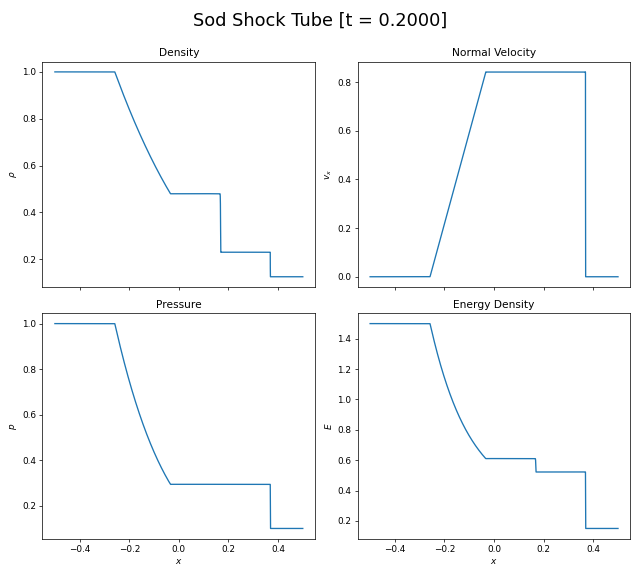
\includegraphics[width=\textwidth]{../Examples/1D/Sod/Sod.png}
\caption{Sod}
\end{subfigure}
\hfill
\begin{subfigure}[t]{0.48\textwidth}
\centering
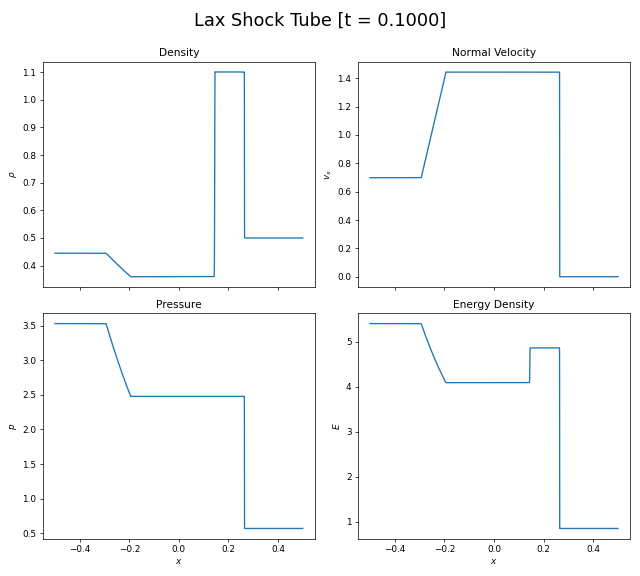
\includegraphics[width=\textwidth]{../Examples/1D/Lax/Lax.png}
\caption{Lax}
\end{subfigure}

\vspace{1em}
\begin{subfigure}[t]{0.48\textwidth}
\centering
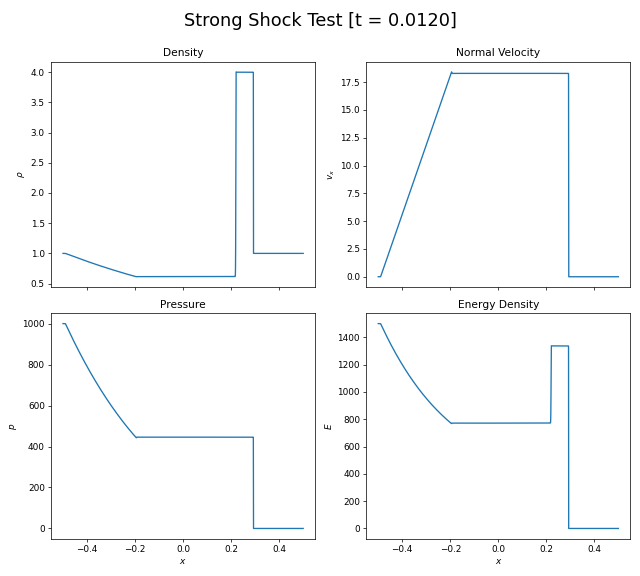
\includegraphics[width=\textwidth]{../Examples/1D/Strong Shock/StrongShock.png}
\caption{Strong Shock}
\end{subfigure}
\hfill
\begin{subfigure}[t]{0.48\textwidth}
\centering
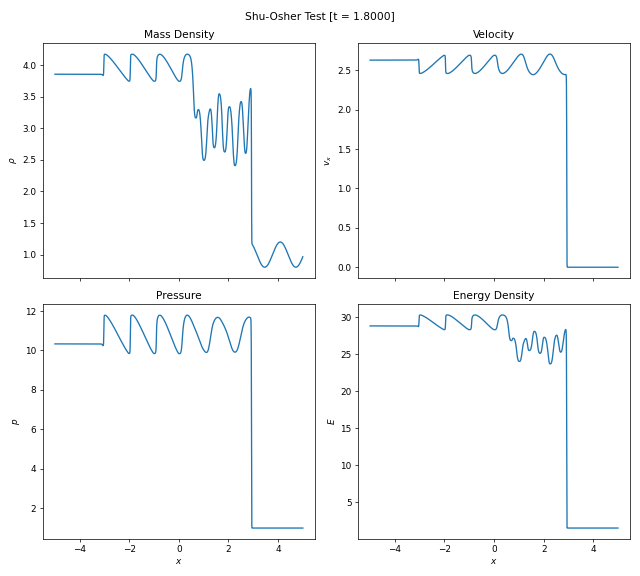
\includegraphics[width=\textwidth]{../Examples/1D/Shu-Osher/Shu & Osher.png}
\caption{Shu \& Osher}
\end{subfigure}
\caption{Reference output for the pure-hydrodynamic 1D examples.}
\label{fig:1d-hydro}
\end{figure}


\begin{table}[htbp]
\centering
\footnotesize
\setlength{\tabcolsep}{4pt}
\caption{Initial states for the 1D example problems.}\label{tab:1D}
\label{tab:1d-examples-ic}
\begin{tabular}{@{}ll>{\raggedright\arraybackslash}p{4.3cm}>{\raggedright\arraybackslash}p{3.0cm}>{\raggedright\arraybackslash}p{4.3cm}@{}}
\toprule
Example & MHD & Left state & Both states & Right state \\
\midrule
Sod & No & \mbox{$\rho = 1.0$}, \mbox{$p = 1.0$} & \mbox{$v = 0$} & \mbox{$\rho = 0.125$}, \mbox{$p = 0.1$} \\
Lax & No & \mbox{$\rho = 0.445$}, \mbox{$v_x = 0.698$}, \mbox{$p = 3.528$} & \mbox{$v_y = v_z = 0$} & \mbox{$\rho = 0.5$}, \mbox{$v_x = 0$}, \mbox{$p = 0.571$} \\
Strong Shock & No & \mbox{$p = 1000.0$} & \mbox{$\rho = 1.0$}, \mbox{$v = 0$} & \mbox{$p = 0.01$} \\
Shu \& Osher & No & \mbox{$\rho = 3.857143$}, \mbox{$v_x = 2.629369$}, \mbox{$p = 10.333333$} & \mbox{$v_y = v_z = 0$} & \mbox{$\rho = 1.0 + 0.2\sin(5x)$}, \mbox{$v_x = 0$}, \mbox{$p = 1.0$} \\
Brio \& Wu & Yes & \mbox{$\rho = 1.0$}, \mbox{$p = 1.0$}, \mbox{$B_y = \sqrt{4\pi}$} & \mbox{$v = 0$}, \mbox{$B_x = 0.75\sqrt{4\pi}$}, \mbox{$B_z = 0$} & \mbox{$\rho = 0.125$}, \mbox{$p = 0.1$}, \mbox{$B_y = -\sqrt{4\pi}$} \\
Dai \& Woodward & Yes & \mbox{$\rho = 1.08$}, \mbox{$v = (1.2, 0.01, 0.5)$}, \mbox{$p = 0.95$}, \mbox{$B_y = 3.6$} & \mbox{$B_x = 2.0$}, \mbox{$B_z = 2.0$} & \mbox{$\rho = 1.0$}, \mbox{$v = (0,0,0)$}, \mbox{$p = 1.0$}, \mbox{$B_y = 4.0$} \\
Ryu \& Jones & Yes & \mbox{$v_x = 10.0$}, \mbox{$p = 20.0$} & \mbox{$\rho = 1.0$}, \mbox{$v_y = v_z = 0$}, \mbox{$B = (5,5,0)$} & \mbox{$v_x = -10.0$}, \mbox{$p = 1.0$} \\
\bottomrule
\end{tabular}
\end{table}

The 1D examples (\bash{Examples/1D/}) are classic shock-tube and wave-interaction Riemann problems with well-established reference solutions:  \citet{Sod1978},  \citet{Lax1954},  \citet{ShuOsher1989}, and the Strong Shock test for pure hydrodynamics; and \citet{BrioWu1988}, citet{DaiWoodward1994}, and \citet{RyuJones1995} for MHD. Each is a self-contained \bash{Config.h}/\bash{Problem.cpp} pair (plus, for Brio \& Wu, a \bash{Constants.h} setting $\gamma = 2$). All of these problems use outflow boundaries, HLLC (hydro) or HLLD (MHD) as the Riemann solver, and MC limiting for hydro / MINMOD for MHD -- MC was found to produce spurious oscillations near strong shocks in the MHD cases. The specific inputs  for each test are listed in \Cref{tab:1D}. \Cref{fig:1d-hydro} shows DRAGON's output for the hydrodynamic problems, generated with DRAGONGAZE (\Cref{ch:gaze}); the corresponding plots for the MHD problems can be found in Appendix \ref{ch:additional-figures}. \Cref{tab:1d-examples-ic} lists the initial left, right, and shared states set up in each problem's \bash{Problem.cpp}.


\subsection{Hydrodynamic Examples in Two and Three dimensions}

The multidimensional hydrodynamic examples (\bash{Examples/Hydro/}) move past 1D shock tubes to exercise genuinely multidimensional behaviour.%: an exactly-known advected solution, a radially symmetric explosion, and a shear instability with no closed-form solution at all. 
For these examples it is of particular importance to exercise the CTU integration (\Cref{sec:ctu}), since the hydrodynamic 12-solve code path is distinct from MHD's 6-solve algorithm. Each example provides a \bash{Problem2D.cpp}; some tests also provide a \bash{Problem3D.cpp} so the same physical setup can be run in either dimensionality.

\subsubsection{Diagonal Advection Test}
\label{sec:diagonal-advection}

Diagonal Advection is DRAGON's simplest convergence test: a smooth sinusoidal density perturbation, $\rho(x,y,0) = \rho_0 + \rho_1\sin\!\big(2\pi(x+y)\big)$, is advected at unit velocity along the grid diagonal ($\mathbf{v} = (1,1)$ in 2D, $(1,1,1)$ in 3D). 
Because the flow is smooth, periodic, and uniform-velocity advection, we can compare the computed solution to the  exact analytic solution 
\begin{equation}\rho_\mathrm{exact}(x,y,t) = \rho_0 + \rho_1\sin\!\big(2\pi(x+y-2t)\big)\end{equation}
 in 2D (and analogously with a $3t$ phase shift in 3D).
We have run this problem using HLLC (\Cref{sec:riemann}) paired with three different limiters (\Cref{sec:reconstruction}) in 2D, plus one 3D run. The results are presented in Tables \ref{tab:diag-2D-minmod}--\ref{tab:diag-3D-MC}.

\begin{table}[htbp]
\centering
\caption{Diagonal Advection  (2D) convergence, HLLC + Minmod.}
\label{tab:diag-2D-minmod}
\begin{tabular}{rcccccc}
\toprule
$n$ & $L_1$ error & $L_1$ rate & $L_2$ error & $L_2$ rate & $L_\infty$ error & $L_\infty$ rate \\
\midrule
128 & $1.034\times10^{-3}$ & --   & $1.412\times10^{-3}$ & --   & $3.703\times10^{-3}$ & --   \\
256 & $2.863\times10^{-4}$ & 1.85 & $4.494\times10^{-4}$ & 1.65 & $1.512\times10^{-3}$ & 1.29 \\
512 & $7.834\times10^{-5}$ & 1.87 & $1.422\times10^{-4}$ & 1.66 & $6.103\times10^{-4}$ & 1.31 \\
\bottomrule
\end{tabular}
\end{table}

\begin{table}[htbp]
\centering
\caption{Diagonal Advection  (2D) convergence, HLLC + MC.}
\label{tab:diag-2D-MC}
\begin{tabular}{rcccccc}
\toprule
$n$ & $L_1$ error & $L_1$ rate & $L_2$ error & $L_2$ rate & $L_\infty$ error & $L_\infty$ rate \\
\midrule
128 & $2.249\times10^{-4}$ & --   & $3.107\times10^{-4}$ & --   & $9.426\times10^{-4}$ & --   \\
256 & $5.631\times10^{-5}$ & 2.00 & $9.315\times10^{-5}$ & 1.74 & $3.880\times10^{-4}$ & 1.28 \\
512 & $1.407\times10^{-5}$ & 2.00 & $2.812\times10^{-5}$ & 1.73 & $1.593\times10^{-4}$ & 1.28 \\
\bottomrule
\end{tabular}
\end{table}

\begin{table}[htbp]
\centering
\caption{Diagonal Advection  (2D) convergence,  HLLC + Superbee.}
\label{tab:diag-2D-superbee}
\begin{tabular}{rcccccc}
\toprule
$n$ & $L_1$ error & $L_1$ rate & $L_2$ error & $L_2$ rate & $L_\infty$ error & $L_\infty$ rate \\
\midrule
128 & $6.932\times10^{-4}$ & --   & $9.097\times10^{-4}$ & --   & $2.784\times10^{-3}$ & --   \\
256 & $1.987\times10^{-4}$ & 1.80 & $2.922\times10^{-4}$ & 1.64 & $1.272\times10^{-3}$ & 1.13 \\
512 & $5.302\times10^{-5}$ & 1.90 & $9.130\times10^{-5}$ & 1.68 & $5.151\times10^{-4}$ & 1.30 \\
\bottomrule
\end{tabular}
\end{table}

\begin{table}[htbp]
\centering
\caption{Diagonal Advection  (3D) convergence,  HLLC + MC.}
\label{tab:diag-3D-MC}
\begin{tabular}{rcccccc}
\toprule
$n$ & $L_1$ error & $L_1$ rate & $L_2$ error & $L_2$ rate & $L_\infty$ error & $L_\infty$ rate \\
\midrule
64  & $1.168\times10^{-3}$ & --   & $1.390\times10^{-3}$ & --   & $2.910\times10^{-3}$ & --   \\
128 & $3.215\times10^{-4}$ & 1.86 & $4.245\times10^{-4}$ & 1.71 & $1.219\times10^{-3}$ & 1.25 \\
256 & $8.195\times10^{-5}$ & 1.97 & $1.283\times10^{-4}$ & 1.73 & $5.142\times10^{-4}$ & 1.25 \\
\bottomrule
\end{tabular}
\end{table}

The data is broadly consistent with the second-order expectation: $L_1$ converges at $q\approx1.9$--$2.0$ for the two smoother limiters (MC, minmod), $L_2$ and $L_\infty$ converge more slowly since they weight the (still slightly under-resolved) peak of the sine wave more heavily.
Superbee meanwhile converges somewhat worse than the other limiters. This is expected, as it is the most compressive of the three limiters, and for a smooth-flow test there is no shock to sharpen so it only adds unnecessary numerical dissipation.

\subsubsection{Sedov Blast Test}
\label{sec:sedov-blast}

The Sedov Blast test deposits a fixed amount of energy $E_\mathrm{blast}$ into a small region of radius $r_0$ (a handful of cells wide) at the centre of an otherwise uniform, low-pressure ambient medium. 
The resulting point explosion is then allowed to expand outward. 
Concretely, this is implemented as a pressure spike: \cpp{Problem::makeProblem()} first counts how many cells actually fall within $r_0$ of the origin at the chosen resolution, then scales the per-cell blast pressure so that the total deposited energy is (to grid resolution) independent of $n$. \cpp{Problem::initialFluidState(...)} then applies that pressure only within $r_0$, leaving density uniform ($\rho=1$) and the exterior at the low ambient pressure $p_\mathrm{amb}=10^{-5}$ everywhere else. 
%The domain uses outflow boundaries (\Cref{sec:boundary}) so the resulting shock can leave the grid without reflecting back in.

The expected result of this problem is the self-similar Sedov--Taylor blast wave \citep{Taylor1950,Sedov1959}: a thin, strong spherical (circular, in 2D) shock expanding outward, enclosing a hot, nearly-uniform-pressure interior and leaving vacuum-like ambient conditions untouched ahead of the shock front. However, such a strong, grid-aligned shock is prone to the carbuncle instability \citep{Quirk1994}, a well-known failure mode in which a contact-preserving solver like HLLC lets a spurious, grid-aligned perturbation grow along the shock front.
To avoid this, we use the HLLE (\Cref{sec:HLLE})  Riemann solver rather than HLLC for this example. HLLE has no separate contact wave, so it is more diffusive across contacts; that extra diffusion is exactly what damps the carbuncle-forming perturbation, at the cost of a somewhat more smeared shock front.

\begin{figure}[htbp]
\centering
\begin{subfigure}[t]{0.48\textwidth}
\centering
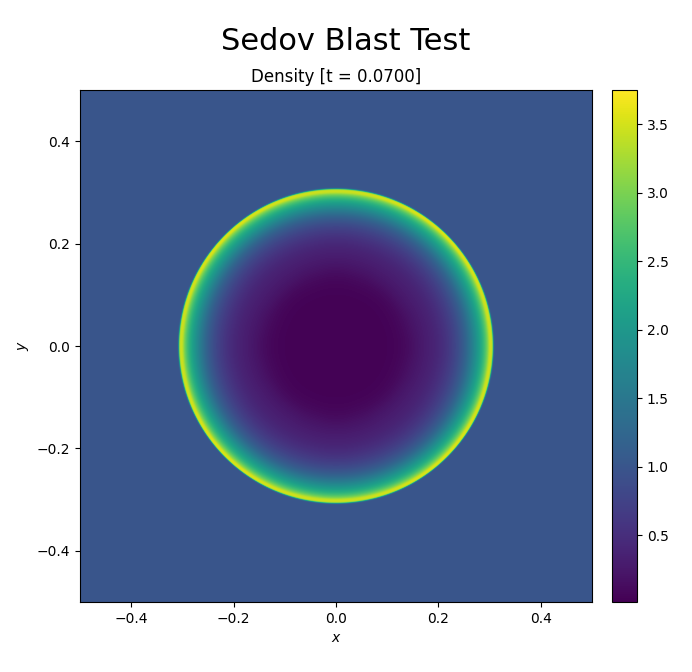
\includegraphics[width=\textwidth]{../Examples/Hydro/Blast/Output - 2D/density_frame_00007.png}
\caption{Density}
\end{subfigure}
\hfill
\begin{subfigure}[t]{0.48\textwidth}
\centering
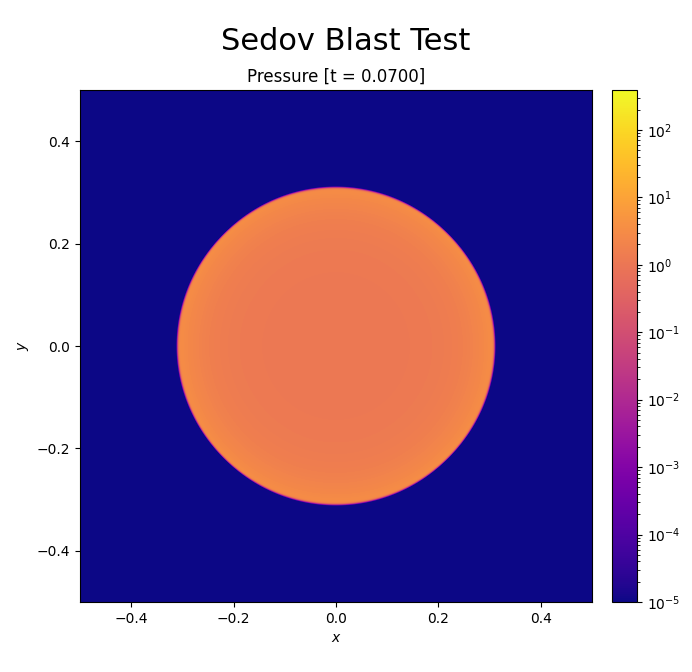
\includegraphics[width=\textwidth]{../Examples/Hydro/Blast/Output - 2D/pressure_frame_00007.png}
\caption{Pressure (log scale)}
\end{subfigure}
\caption{Reference output for the 2D Sedov Blast test at $t=0.07$.}
\label{fig:blast}
\end{figure}

The results plotted in \Cref{fig:blast} are as expected:  
the density panel shows the characteristic thin high-density shell trailing the shock front with a nearly-evacuated interior, 
and the (log-scaled) pressure panel shows the sharp several-orders-of-magnitude jump across the shock separating the hot post-shock bubble from the undisturbed ambient medium. 


\subsubsection{Kelvin--Helmholtz Instability}
\label{sec:kh-instability}

The Kelvin--Helmholtz example sets up a shear layer, following the well-posed construction of \citet{McNallyLyraPassy2012}: a denser right moving band ($\rho_1=2$, $v_x = +V_0$) separated from a lighter left-moving ambient medium ($\rho_2=1, v_x = -V_0$) by two $\tanh$-smoothed interfaces.
A small, spatially-localized transverse velocity perturbation is seeded at both interfaces -- a $\sin(2\pi\,\mathtt{kmode}\,x)$ pattern windowed by a Gaussian centred on each interface; this gives the shear instability something to grow from rather than waiting on grid noise.
Two passive scalars are used to trace the fluid: one is initialised to 1 in the upper ambient region and 0 everywhere else, and the other likewise in the lower ambient region.


\begin{figure}[htbp]
\centering
\begin{subfigure}[t]{0.48\textwidth}
\centering
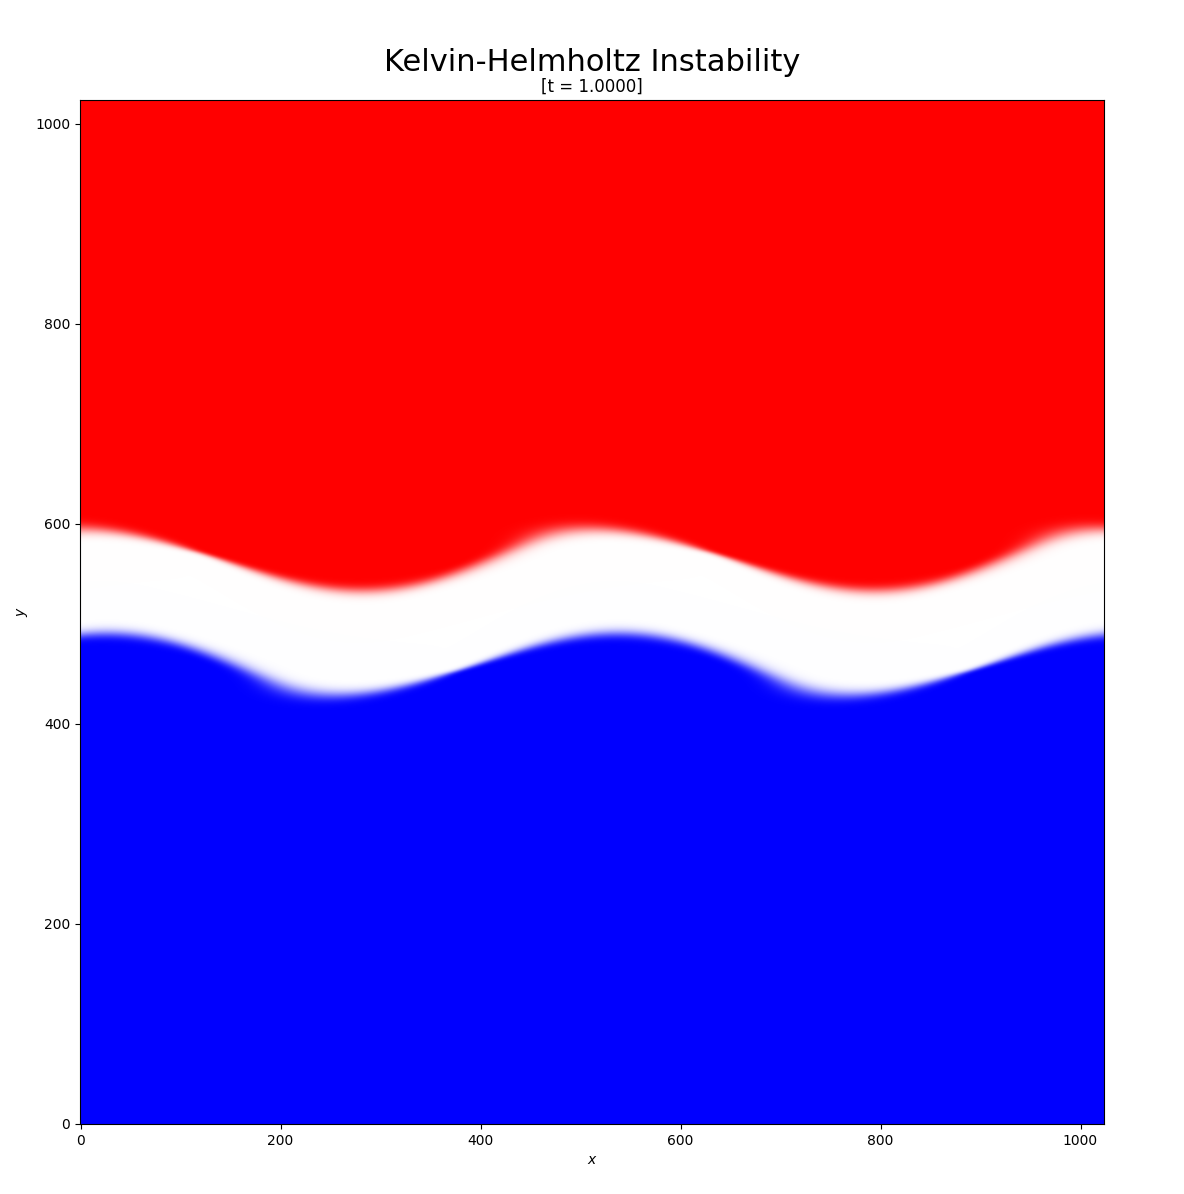
\includegraphics[width=\textwidth]{../Examples/Hydro/Kelvin-Helmholtz/Outputs/KH_t_1_0.png}
\caption{$t=1.0$}
\end{subfigure}
\hfill
\begin{subfigure}[t]{0.48\textwidth}
\centering
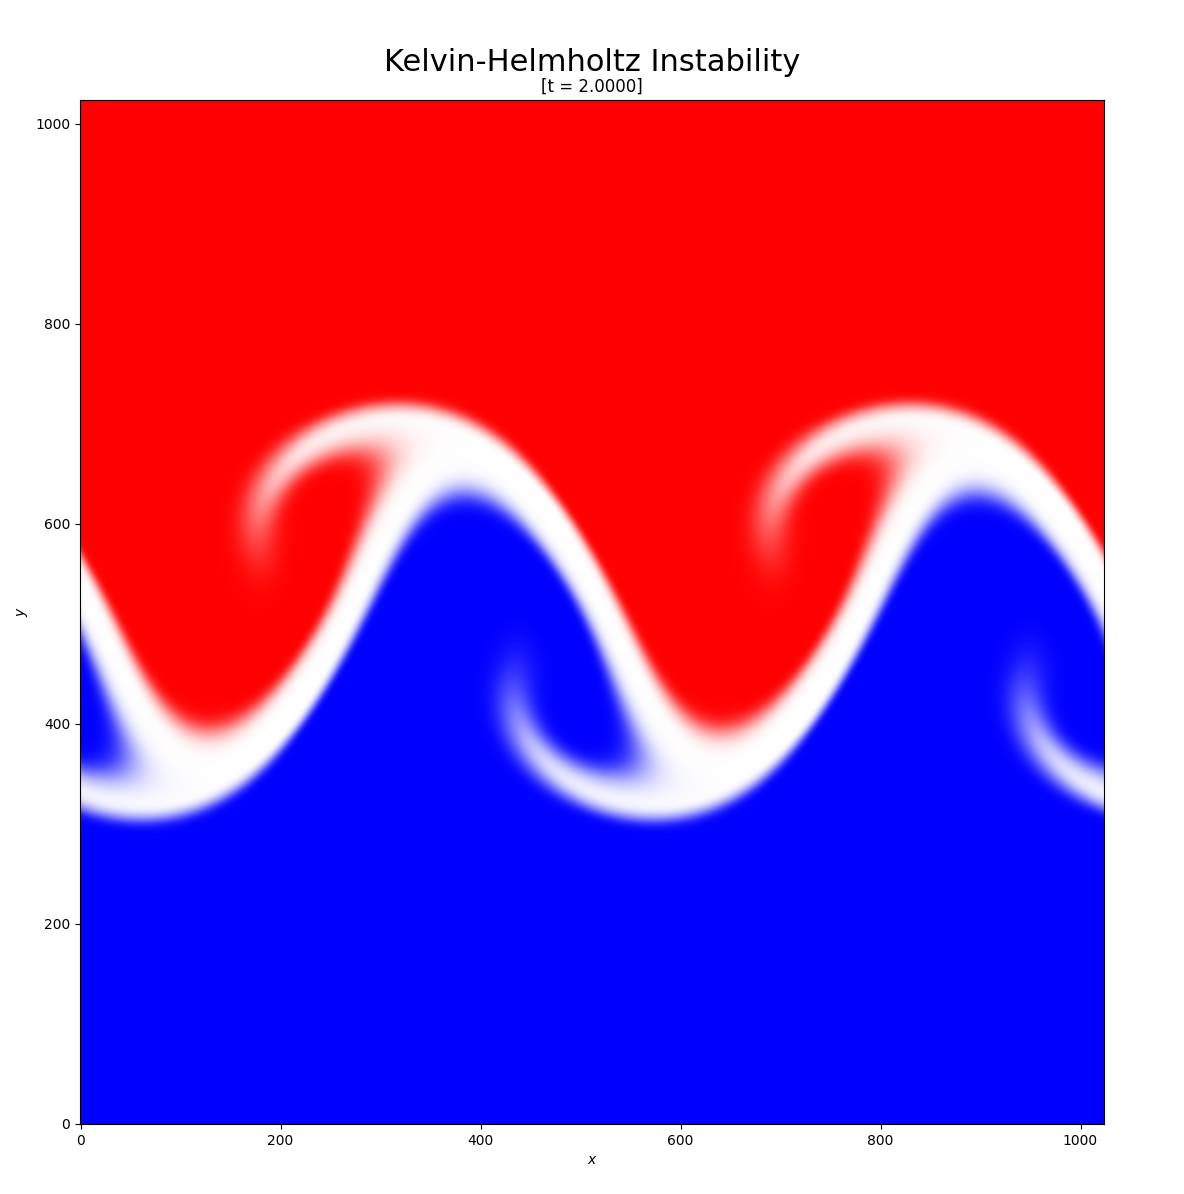
\includegraphics[width=\textwidth]{../Examples/Hydro/Kelvin-Helmholtz/Outputs/KH_t_2_0.png}
\caption{$t=2.0$}
\end{subfigure}
\caption{A heatmap of two tracers, showing the growth of the Kelvin--Helmholtz instability.}
\label{fig:kh}
\end{figure}


Unlike the other two examples in this section, Kelvin--Helmholtz has no closed-form solution to compare against -- growth of the shear instability is chaotic at late times, so this example is checked qualitatively, by confirming the characteristic vortex roll-up pattern appears and grows as expected. \Cref{fig:kh} shows this development: at $t=1$ the perturbation is still a small-amplitude wave on the shear interface, while by $t=2$ it has rolled up into the pair of vortices expected from \cpp{kmode=2} (one every half-period of the seeded perturbation), with visible secondary structure at the vortex cores from the instability continuing to cascade to smaller scales.



\subsection{MHD Examples in Two and Three dimensions}
\subsubsection{Field Loop Advection}
\label{sec:loop-advection}

The field loop advection test \citep{GardinerStone2005,GardinerStone2008} carries a weak magnetic field loop across a periodic domain at uniform velocity.
The field is deliberately weak ($B_0=10^{-6}$) in order to isolate inductive advection from the effects of magnetic pressure and tension altering the fluid.
Any distortion, diffusion, or divergence error in the transported field can only come from the induction step itself. 
The background velocity is oblique to all grid axes: $(v_x,v_y)=(2,0.5)$ in 2D and $(v_x,v_y,v_z)=(2,1,1)$ in 3D (with the loop uniform in the $z$ direction).

The example problem supports two loop profiles. The \emph{uniform} profile sets the vector potential $A_z = B_0\max(r_0-r,0)$, a cone that is linear in $r$ and therefore gives a field of constant magnitude $|B_\phi|=B_0$ everywhere inside $r<r_0$, dropping to zero outside. The \emph{Gaussian} profile instead sets $A_z=B_0\exp\!\big(-\tfrac12(r/r_0)^2\big)$, giving a smooth field magnitude that peaks in an annulus around the loop centre and has no kink.

Because the domain is periodic and the advection velocity is uniform, the chosen run time is an integer number of periods along all axes, so the field should return exactly to its initial shape.
 \Cref{fig:loop-advection} shows this for both profiles, both at the initial and final times.

\begin{figure}[htbp]
\centering
\begin{subfigure}[t]{0.48\textwidth}
\centering
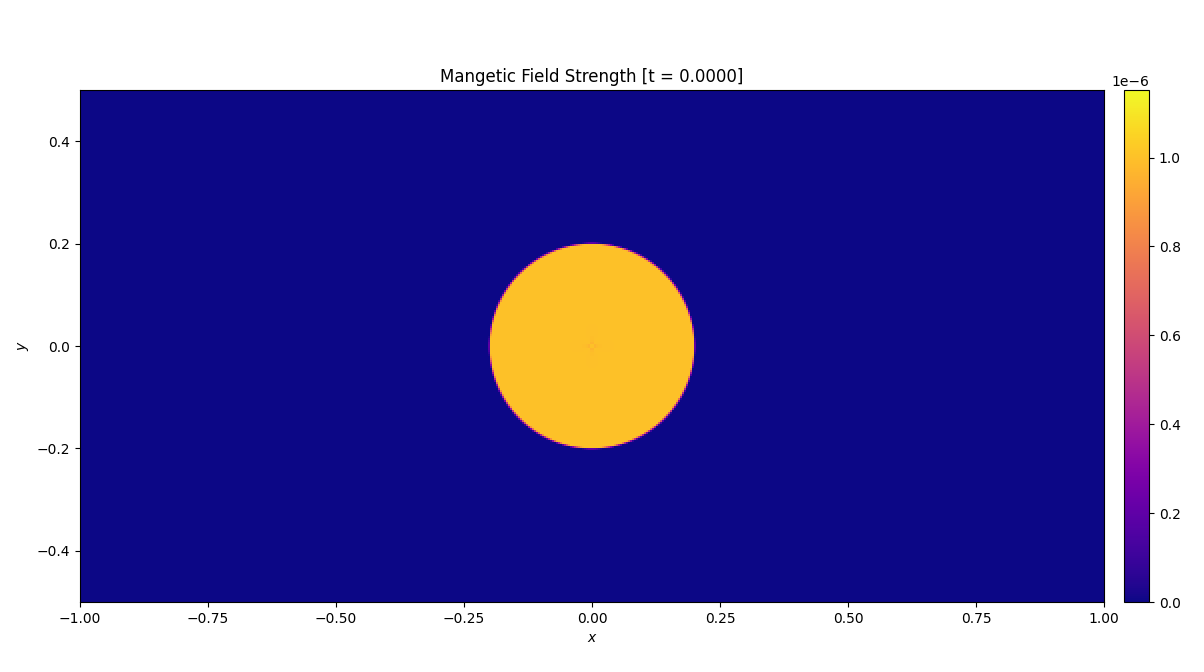
\includegraphics[width=\textwidth]{../Examples/MHD/LoopAdvection/Outputs/2D_frame_0.png}
\caption{2D, uniform $B_\phi$, $t=0$}
\end{subfigure}
\hfill
\begin{subfigure}[t]{0.48\textwidth}
\centering
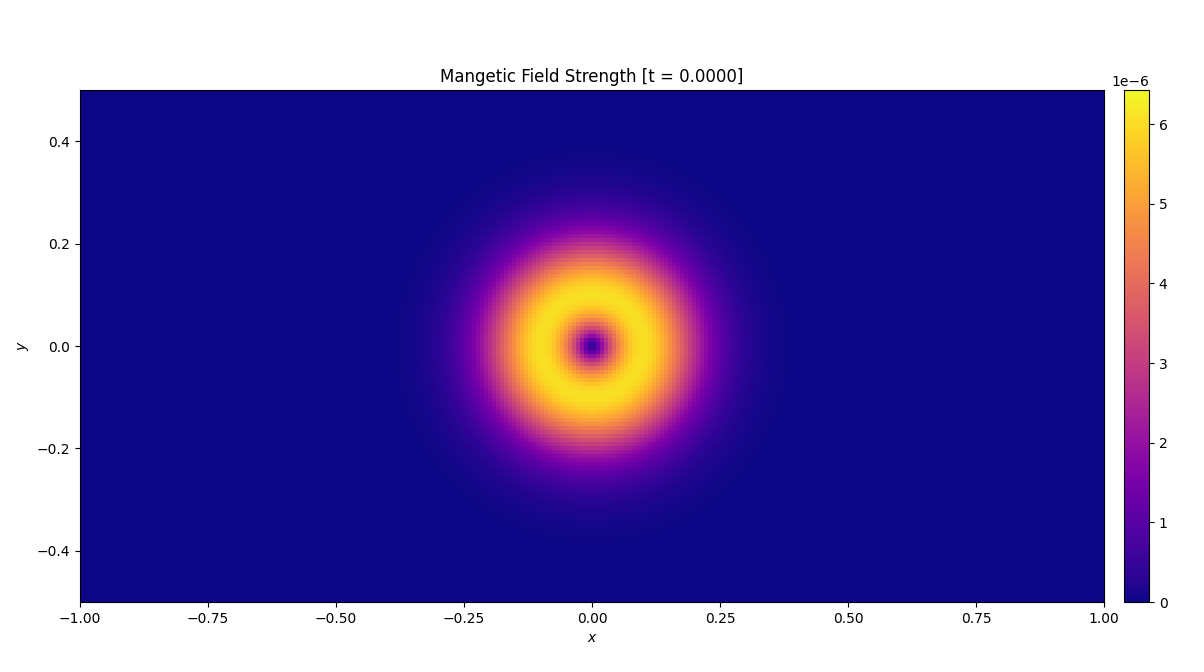
\includegraphics[width=\textwidth]{../Examples/MHD/LoopAdvection/Outputs/3D_Gaussian_0.png}
\caption{3D, Gaussian $A_z$, $t=0$}
\end{subfigure}

\begin{subfigure}[t]{0.48\textwidth}
\centering
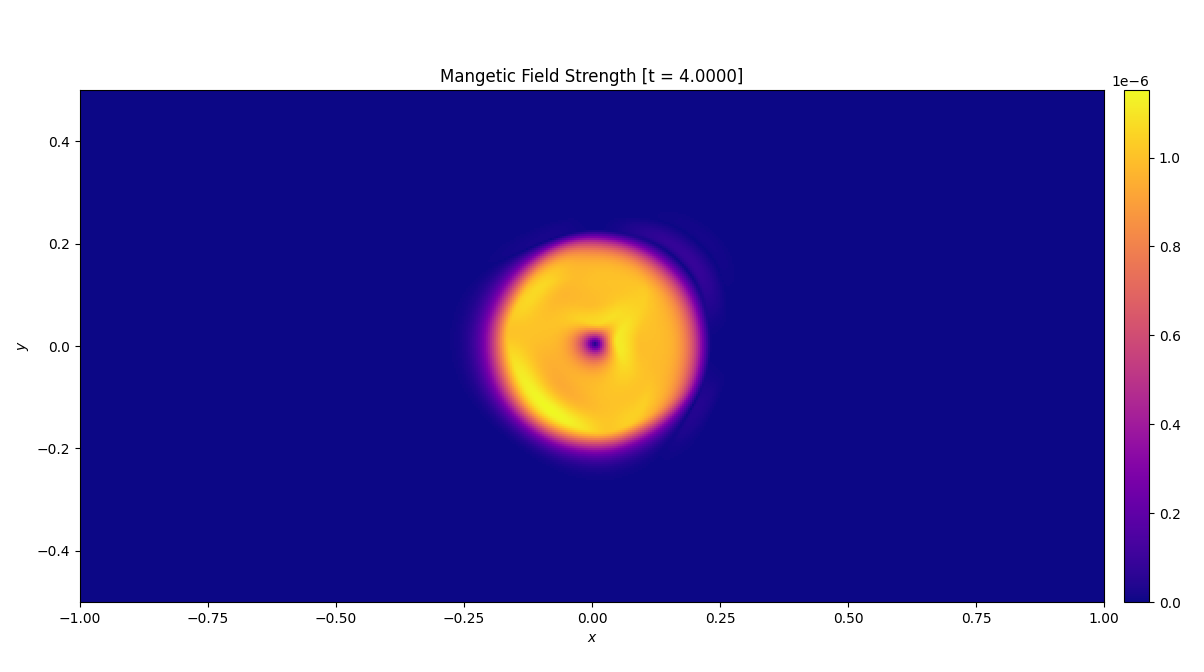
\includegraphics[width=\textwidth]{../Examples/MHD/LoopAdvection/Outputs/2D_frame_40.png}
\caption{2D, uniform $B_\phi$, $t=4$}
\end{subfigure}
\hfill
\begin{subfigure}[t]{0.48\textwidth}
\centering
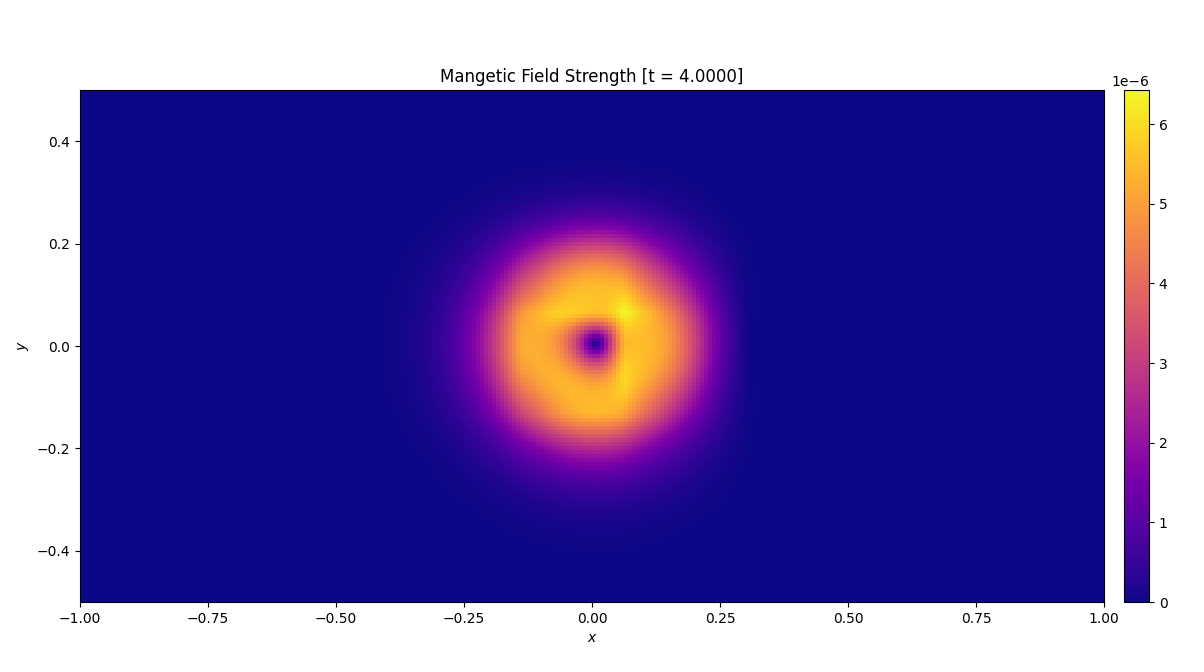
\includegraphics[width=\textwidth]{../Examples/MHD/LoopAdvection/Outputs/3D_Gaussian_40.png}
\caption{3D, Gaussian $A_z$, $t=4$}
\end{subfigure}
\caption{Magnetic field strength for the Field Loop Advection test, before and after two full advection periods.}
\label{fig:loop-advection}
\end{figure}

As with the other periodic advection tests, \cpp{Problem::problemComplete(...)} validates the run by reloading the initial frame from disk with \cpp{DRAGONHOARD::loadFromFile(...)} and differencing it against the final state, componentwise in $\mathbf{B}$. 
The reported $L_1$ error is $|\overline{\delta\mathbf B}|$, the magnitude of the mean absolute error vector.
Convergence data for both profiles are given in \Cref{tab:loop-uniform}--\Cref{tab:loop-gaussian}. The $n=512$ cases were not run in 3D on account of the diminishing returns for another high-resolution simulation being insufficient to justify the multi-day runtime.

\begin{table}[htbp]
\centering
\caption{Field Loop Advection, uniform $B_\phi$ convergence.}
\begin{tabular}{rcccc}
\toprule
& \multicolumn{2}{c}{2D} & \multicolumn{2}{c}{3D} \\
\cmidrule(lr){2-3}\cmidrule(lr){4-5}
$n$ & $L_1$ error & $L_1$ rate & $L_1$ error & $L_1$ rate \\
\midrule
64  & $5.211\times10^{-8}$ & --   & $5.657\times10^{-8}$ & --   \\
128 & $2.718\times10^{-8}$ & 0.94 & $3.040\times10^{-8}$ & 0.90 \\
256 & $1.615\times10^{-8}$ & 0.74 & $1.771\times10^{-8}$ & 0.78   \\
512 & $1.052\times10^{-8}$ & 0.62 & --                   & --   \\
\bottomrule
\end{tabular}
\label{tab:loop-uniform}
\end{table}

\begin{table}[htbp]
\centering
\caption{Field Loop Advection, Gaussian $A_z$ convergence.}
\begin{tabular}{rcccc}
\toprule
& \multicolumn{2}{c}{2D} & \multicolumn{2}{c}{3D} \\
\cmidrule(lr){2-3}\cmidrule(lr){4-5}
$n$ & $L_1$ error & $L_1$ rate & $L_1$ error & $L_1$ rate \\
\midrule
64  & $2.088\times10^{-7}$ & --   & $2.309\times10^{-7}$ & --   \\
128 & $8.032\times10^{-8}$ & 1.38 & $9.191\times10^{-8}$ & 1.32 \\
256 & $2.702\times10^{-8}$ & 1.57 & $3.214\times10^{-8}$ & 1.51 \\
512 & $9.061\times10^{-9}$ & 1.57 & --                   & --   \\
\bottomrule
\end{tabular}
\label{tab:loop-gaussian}
\end{table}

Unlike Diagonal Advection (\Cref{sec:diagonal-advection}), which converges at $q\approx1.9$--$2.0$, the loop advection error rates sit well below second order: $q\approx0.6$--$0.9$ for the uniform-$B_\phi$ profile and $q\approx1.3$--$1.6$ for the Gaussian profile. 
For the uniform-$B_\phi$ profile, this is most likely the result of the discontinuities at $r=0$ and $r_0$:  a scheme built around smooth reconstruction cannot converge faster than first order through a kink like this, which caps its observed rate close to 1. 
The Gaussian profile has no such kink and converges noticeably faster, though it is still below the $q\approx2$ seen for Diagonal Advection. %This may be a result of the loop being a genuinely two-dimensional feature  as opposed to Diagonal Advection's sine wave being separable and effectively one-dimensional along the advection direction. 

\subsubsection{Linear Wave Convergence}
\label{sec:linear-waves}

The MHD linear wave test \citep{GardinerStone2008} seeds a single, exactly linear eigenmode of the MHD equations on top of a uniform background state and lets it propagate.
The background is oriented obliquely to the grid so that the wave crosses all three axes rather than propagating along a single grid line, allowing this problem to properly test the convergence of DRAGON's CTU-CT implementation.

All seven wave modes are implemented: fast, Alfv\'en, slow, and entropy, with $+$ and $-$ variants for the first three.
 The background is perturbed by $\epsilon R\cos(2\pi x_1)$, where $R$ is the analytic eigenvector for the selected mode, $x_1$ is the rotated propagation coordinate, and $\epsilon=10^{-6}$ is small enough to stay in the linear regime.

As with Field Loop Advection, validation reloads the initial frame with \cpp{DRAGONHOARD::loadFromFile(...)} and differences it against the state after the wave has propagated an integer number of wavelengths back to its starting position. Here the comparison spans every conserved field at once: the componentwise $L_1$ errors in $\rho$, $\rho\mathbf{v}$, $\mathbf{B}$, and $E$ are all computed, and then combined into a single scalar
\begin{equation}
L_1 = \sqrt{L_1(\rho)^2 + L_1(\rho\mathbf{v})^2 + L_1(\mathbf B)^2 + L_1(E)^2}.
\end{equation}
Tables \ref{tab:wave-fast}--\ref{tab:wave-entropy} give the results for both propagation directions ($+$/$-$) of the fast, Alfv\'en, and slow modes, as well as for the (direction-independent) entropy mode.

\begin{table}[htbp]
\centering
\caption{MHD Linear Wave (3D, fast mode) convergence.}
\begin{tabular}{rcccc}
\toprule
$n$ & $(+)$ $L_1$ error & $(+)$ $L_1$ rate & $(-)$ $L_1$ error & $(-)$ $L_1$ rate \\
\midrule
16 & $5.389\times10^{-7}$ & --   & $5.389\times10^{-7}$ & --   \\
32 & $1.171\times10^{-7}$ & 2.20 & $1.175\times10^{-7}$ & 2.20 \\
64 & $3.466\times10^{-8}$ & 1.76 & $3.463\times10^{-8}$ & 1.76 \\
\bottomrule
\end{tabular}
\label{tab:wave-fast}
\end{table}

\begin{table}[htbp]
\centering
\caption{MHD Linear Wave (3D, Alfv\'en mode) convergence.}
\begin{tabular}{rcccc}
\toprule
$n$ & $(+)$ $L_1$ error & $(+)$ $L_1$ rate & $(-)$ $L_1$ error & $(-)$ $L_1$ rate \\
\midrule
16 & $4.657\times10^{-7}$ & --   & $4.657\times10^{-7}$ & --   \\
32 & $9.576\times10^{-8}$ & 2.28 & $9.573\times10^{-8}$ & 2.28 \\
64 & $2.481\times10^{-8}$ & 1.95 & $2.482\times10^{-8}$ & 1.95 \\
\bottomrule
\end{tabular}
\label{tab:wave-alfven}
\end{table}

\begin{table}[htbp]
\centering
\caption{MHD Linear Wave (3D, slow mode) convergence.}
\begin{tabular}{rcccc}
\toprule
$n$ & $(+)$ $L_1$ error & $(+)$ $L_1$ rate & $(-)$ $L_1$ error & $(-)$ $L_1$ rate \\
\midrule
16 & $1.723\times10^{-7}$ & --   & $1.723\times10^{-7}$ & --   \\
32 & $4.457\times10^{-8}$ & 1.95 & $4.457\times10^{-8}$ & 1.95 \\
64 & $1.321\times10^{-8}$ & 1.75 & $1.322\times10^{-8}$ & 1.75 \\
\bottomrule
\end{tabular}
\label{tab:wave-slow}
\end{table}

\begin{table}[!htbp]
\centering
\caption{MHD Linear Wave (3D, entropy mode) convergence.}
\begin{tabular}{rcc}
\toprule
$n$ & $L_1$ error & $L_1$ rate \\
\midrule
16 & $1.250\times10^{-7}$ & --   \\
32 & $4.511\times10^{-8}$ & 1.47 \\
64 & $1.381\times10^{-8}$ & 1.71 \\
\bottomrule
\end{tabular}
\label{tab:wave-entropy}
\end{table}

The fast, Alfv\'en, and slow modes all converge close to second order at these resolutions, as expected for smooth linear waves on the (formally second-order) MUSCL--Hancock scheme.
The entropy mode converges somewhat more slowly; this mode is purely advected, so its accuracy is governed entirely by the scalar advection error similar in character to the sub-second-order behaviour seen for the piecewise-linear loop profile in \Cref{sec:loop-advection}.
For the fast, Alfv\'en, and slow modes, the  $+$ and $-$ branches agree with each other to within a few percent, as expected by symmetry.



\subsubsection{MHD Blast}
\label{sec:mhd-blast}

The MHD Blast test \citep{GardinerStone2008} is the magnetized counterpart to the hydrodynamic Sedov Blast (\Cref{sec:sedov-blast}): a small central region of radius $r_0$ is set to a much higher pressure ($p_\mathrm{blast}=100$) than the surrounding ambient medium ($p_\mathrm{amb}=1$), with uniform density and zero velocity everywhere. 
Unlike the hydro version, the domain is threaded by a strong, uniform background magnetic field, with magnetic pressure comparable to or larger than the blast overpressure. 
This field is  oriented diagonally at $45^\circ$ to the grid by default to better exercise the CTU machinery.


\begin{figure}[!htbp]
\centering
\begin{subfigure}[t]{0.24\textwidth}
\centering
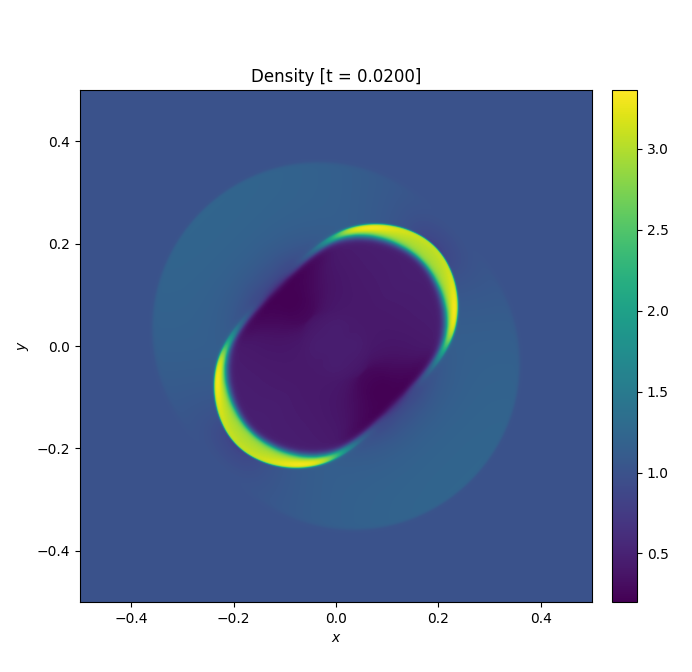
\includegraphics[width=\textwidth]{../Examples/MHD/Blast/Outputs/MHD_Blast_2D_density.png}
\caption{2D, Density}
\end{subfigure}
\hfill
\begin{subfigure}[t]{0.24\textwidth}
\centering
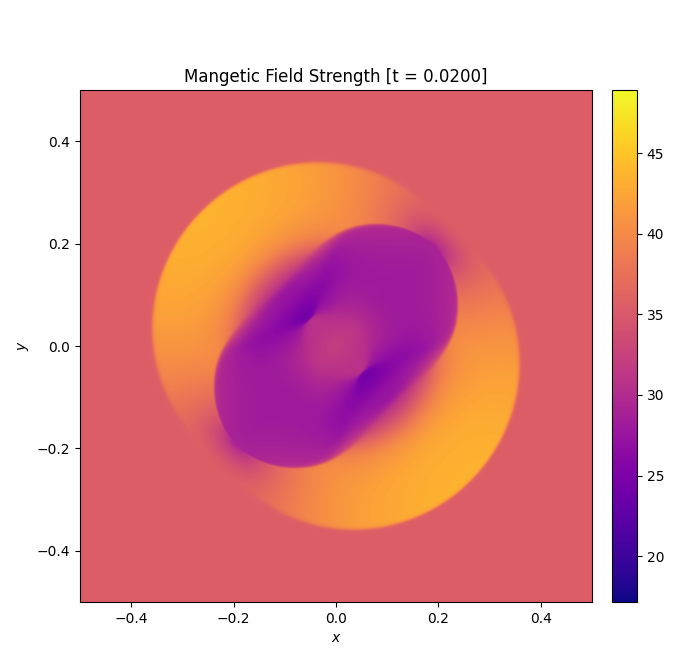
\includegraphics[width=\textwidth]{../Examples/MHD/Blast/Outputs/MHD_Blast_2D_magnetic.png}
\caption{2D, $|\mathbf{B}|$}
\end{subfigure}
\hfill
\begin{subfigure}[t]{0.24\textwidth}
\centering
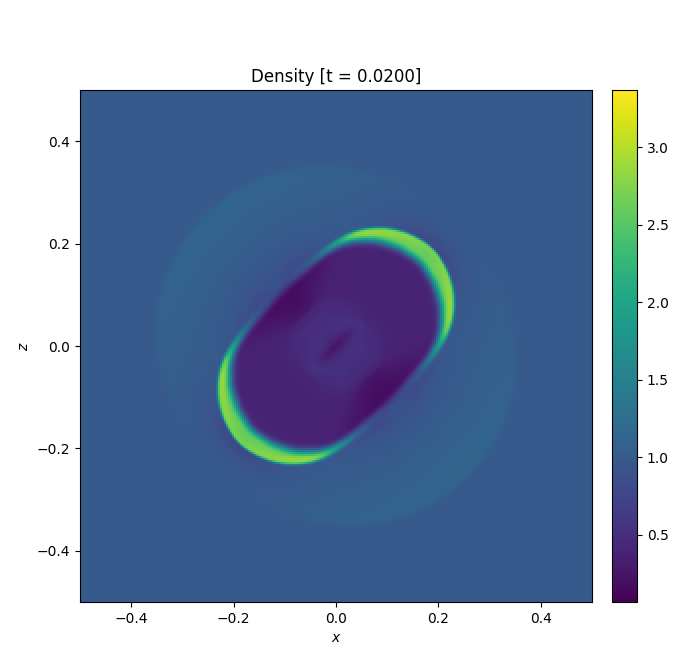
\includegraphics[width=\textwidth]{../Examples/MHD/Blast/Outputs/MHD_Blast_3D_density.png}
\caption{3D, Density}% (mid-plane slice)}
\end{subfigure}
\hfill
\begin{subfigure}[t]{0.24\textwidth}
\centering
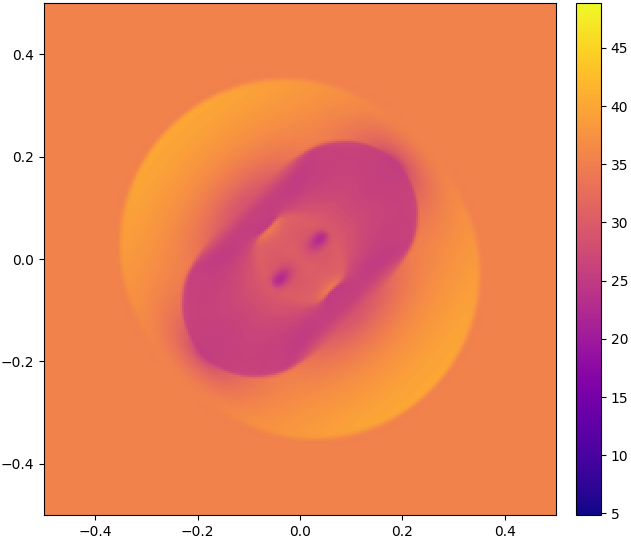
\includegraphics[width=\textwidth]{../Examples/MHD/Blast/Outputs/MHD_Blast_3D_magnetic.png}
\caption{3D, $|\mathbf{B}|$ }%(mid-plane slice)}
\end{subfigure}
\caption{MHD Blast test at $t=0.02$, 2D and 3D (mid-plane slices).}
\label{fig:mhd-blast}
\end{figure}



\Cref{fig:mhd-blast} shows the result in both 2D and 3D. 
As a result of magnetic tension along the field lines, the blast expansion is no longer circular as was the case in the hydrodynamic counterpart. Instead, the anisotropic blast expansion should demonstrate the shock moving faster along the field lines than in other directions. The magnetic field strength panels show evacuated cavities near the blast centre, where the explosion has pushed the field outward and compressed it into the bright rim.


\subsubsection{MHD Rotor}
\label{sec:mhd-rotor}

The MHD Rotor test \citep{BalsaraSpicer1999,Toth2000} embeds a dense, rigidly rotating disk ($\rho_0=10$, angular velocity $\omega=20$, radius $r_0=0.1$) in a lighter, stationary ambient medium ($\rho_\mathrm{amb}=1$), with a linear taper in density and velocity between $r_0$ and $r_1=0.115$ so the initial condition is continuous. A uniform background field $B_x=B_0$ threads the whole domain. 
Though the problem has no closed analytical solution, it is still useful in demonstrating expected behaviours of MHD: 
as the disk spins up the surrounding fluid, it winds the field lines into a strong torsional structure, launching Alfv\'en waves outward and progressively braking the rotor , thus testing the coupling between the magnetic tension force and rotational flow.

\begin{figure}[htbp]
\centering
\begin{subfigure}[t]{0.48\textwidth}
\centering
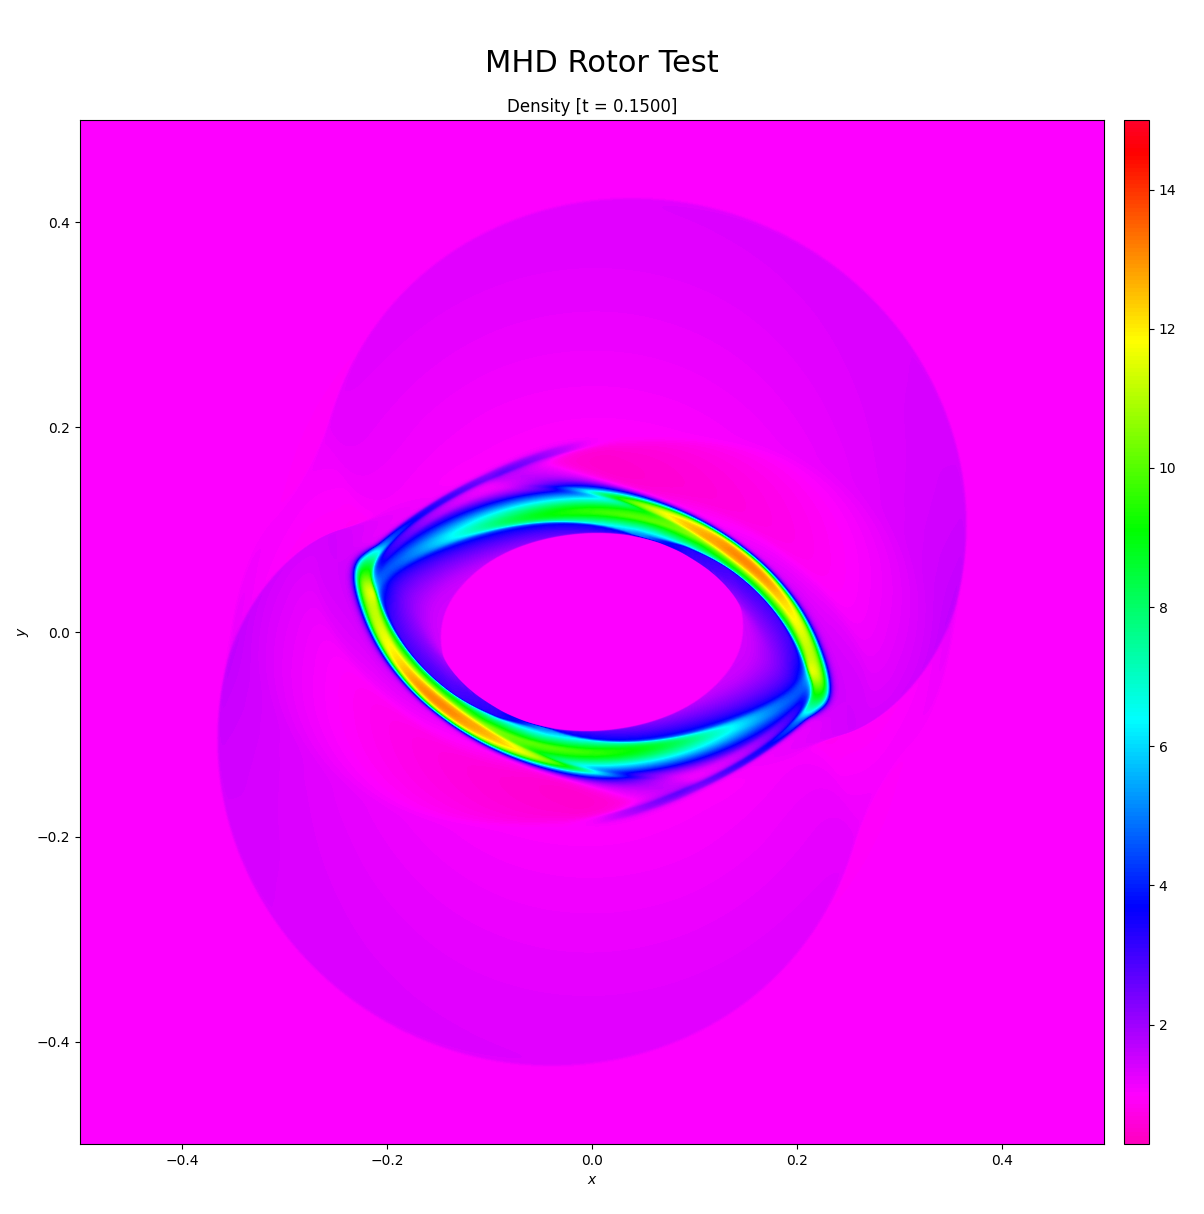
\includegraphics[width=\textwidth]{../Examples/MHD/MHDRotor/Outputs/MHDRotor2D-density.png}
\caption{Density}
\end{subfigure}
\hfill
\begin{subfigure}[t]{0.48\textwidth}
\centering
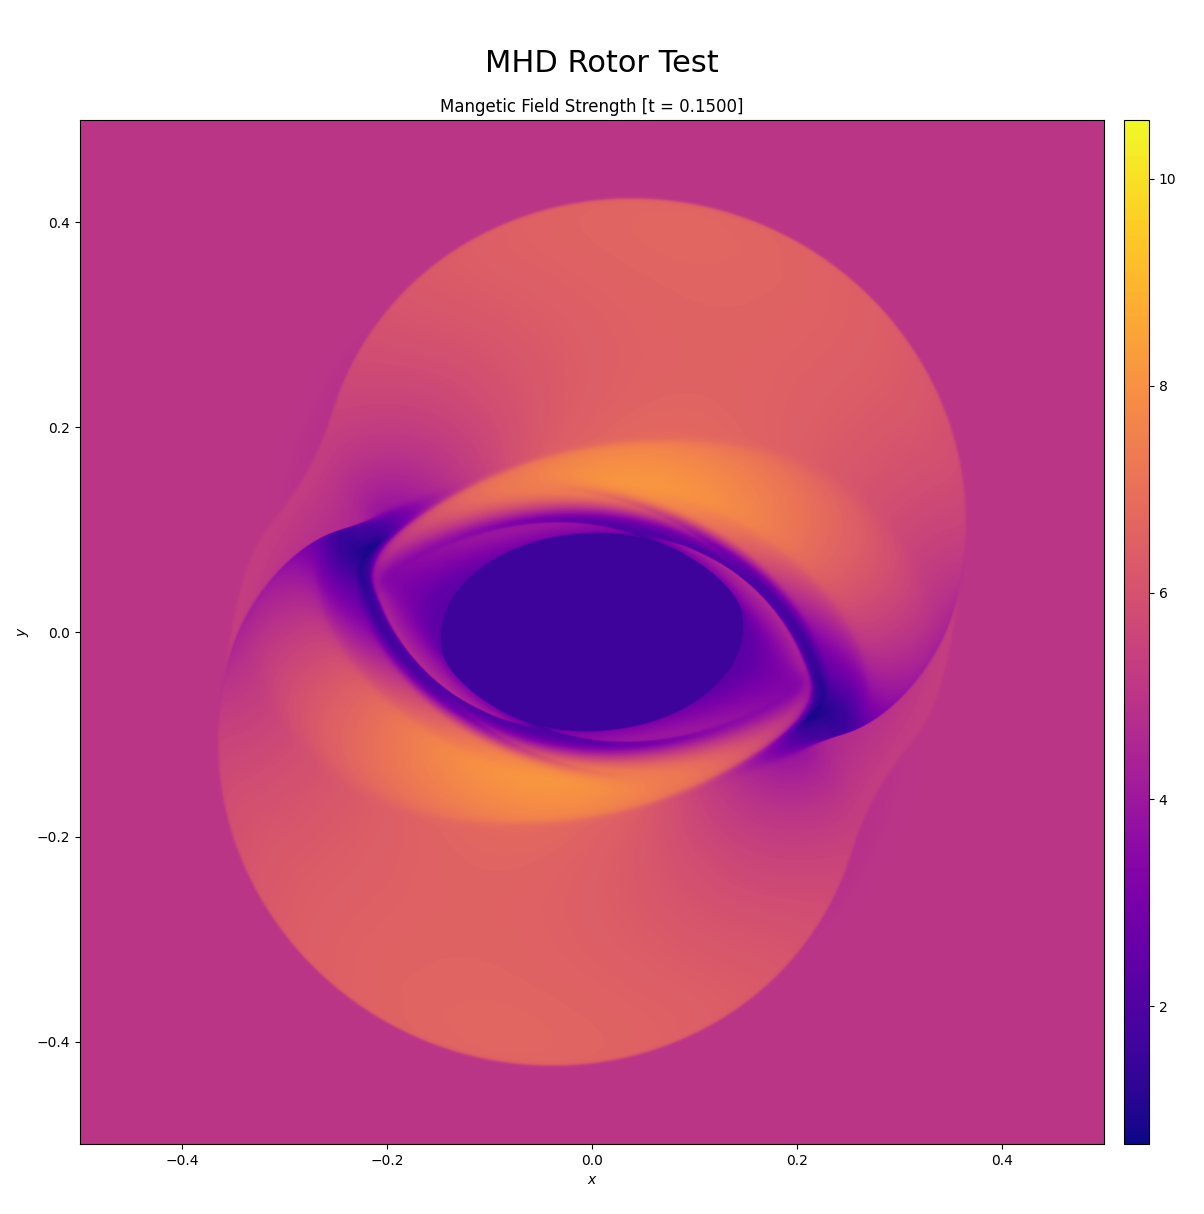
\includegraphics[width=\textwidth]{../Examples/MHD/MHDRotor/Outputs/MHDRotor2D-magnetic.png}
\caption{$|\mathbf{B}|$}
\end{subfigure}
\caption{MHD Rotor test at $t=0.15$.}
\label{fig:mhd-rotor}
\end{figure}


\Cref{fig:mhd-rotor} shows the expected result: the dense rotor has been drawn out into a thin, sheared ring bounded by a pair of spiral shocks, while the magnetic field strength panel shows the low-field cavity carved out at the centre of the rotor and the wound-up, compressed field trailing behind the spiral arms -- the signature of the torsional Alfv\'en waves the rotation launches into the ambient medium.

\subsubsection{Orszag--Tang}
\label{sec:orszag-tang}

The Orszag--Tang vortex \citep{OrszagTang1979} is a fully periodic problem on $[0,2\pi]^2$: the velocity field $\mathbf v = (-\sin y,\ \sin x, 0)$ sets up a large-scale vortical flow, while the vector potential $A_z = B_0\big(\cos y + \tfrac14\cos 2x\big)$ seeds a magnetic field with an X-point current sheet at the origin. As with the MHD Rotor, there is no closed-form solution to compare against; instead this problem is a visual benchmark of a code's ability to handle the development of MHD turbulence, evolving a smooth initial vortex into a cascade of interacting shocks and current sheets.


\begin{figure}[htbp]
\centering
\begin{subfigure}[t]{0.48\textwidth}
\centering
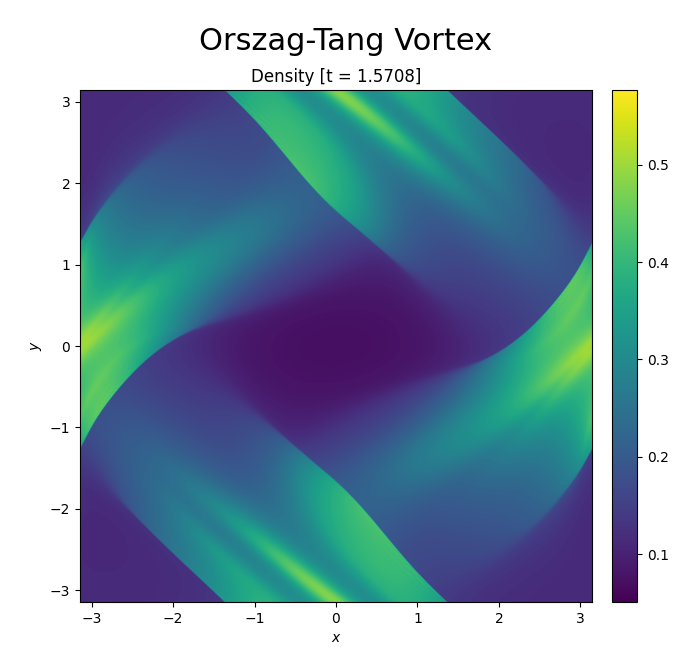
\includegraphics[width=\textwidth]{../Examples/MHD/Orszag–Tang/Outputs/OT2D-1.png}
\caption{$t=\pi/2$}
\end{subfigure}
\hfill
\begin{subfigure}[t]{0.48\textwidth}
\centering
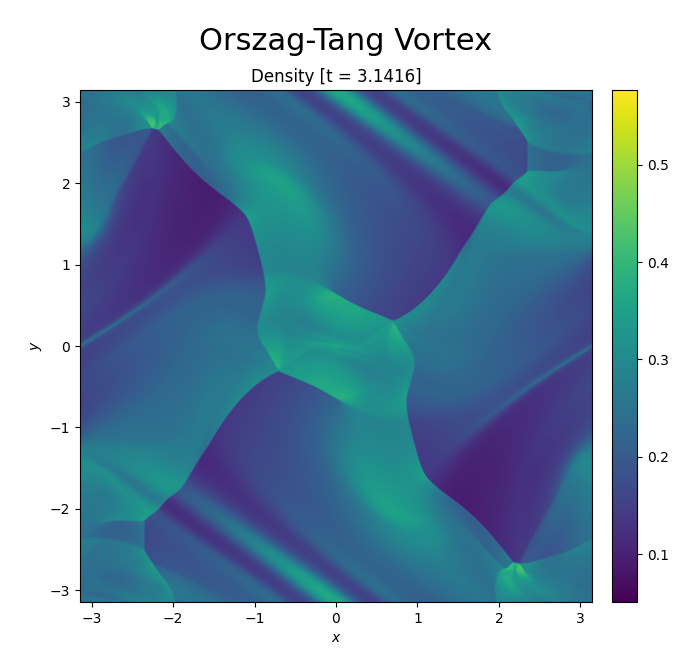
\includegraphics[width=\textwidth]{../Examples/MHD/Orszag–Tang/Outputs/OT2D-2.png}
\caption{$t=\pi$}
\end{subfigure}

\begin{subfigure}[t]{0.48\textwidth}
\centering
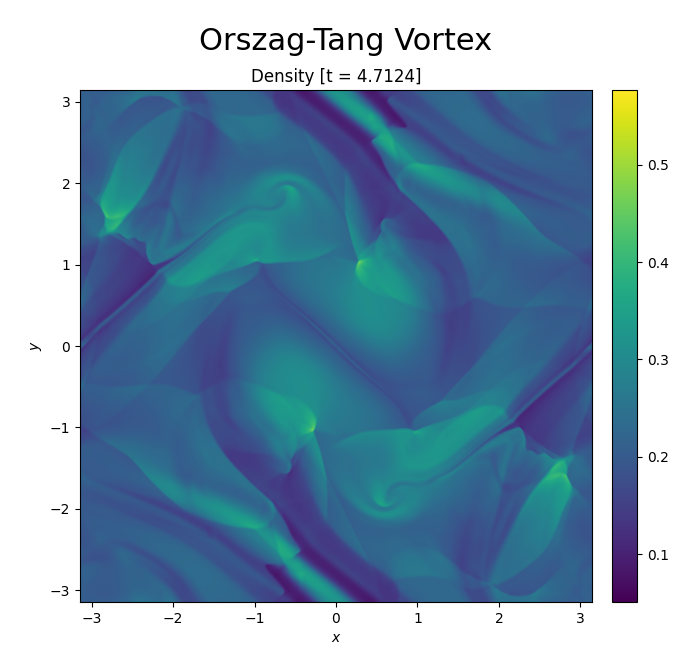
\includegraphics[width=\textwidth]{../Examples/MHD/Orszag–Tang/Outputs/OT2D-3.png}
\caption{$t=3\pi/2$}
\end{subfigure}
\hfill
\begin{subfigure}[t]{0.48\textwidth}
\centering
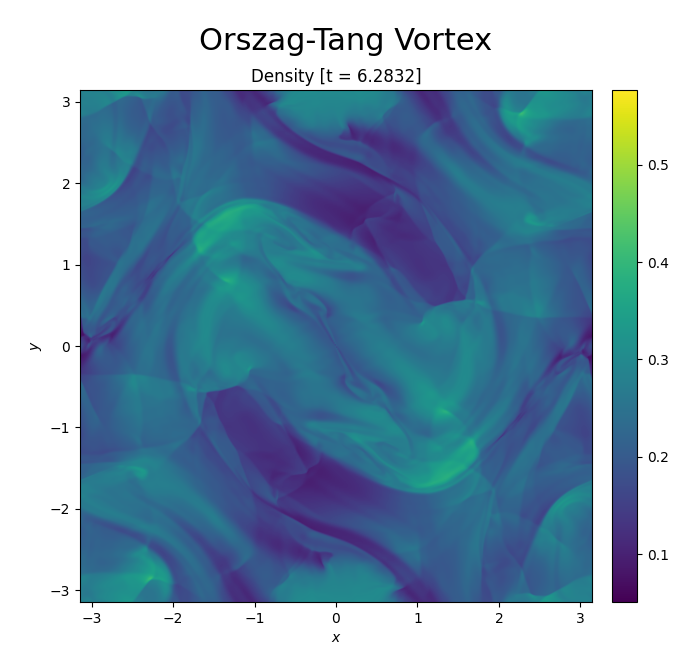
\includegraphics[width=\textwidth]{../Examples/MHD/Orszag–Tang/Outputs/OT2D-4.png}
\caption{$t=2\pi$}
\end{subfigure}
\caption{Density evolution of the Orszag--Tang vortex.}
\label{fig:orszag-tang}
\end{figure}




\Cref{fig:orszag-tang} shows this development.
At $t=\pi/2$, the flow is still close to the smooth initial vortex, with the first diagonal shear bands just beginning to steepen.
By $t=\pi$, these have sharpened into well-defined oblique shocks bracketing the central current sheet.
Finally, at $t=3\pi/2$ and $t=2\pi$ the interacting shocks have broken the flow up into a web of small-scale structure characteristic of MHD turbulence.



% ================= Appendix =================
\appendix

\chapter{Additional Test Problem Plots}
\label{ch:additional-figures}

Full-page versions of the MHD 1D reference plots referenced from \Cref{sec:tests-examples}, one per figure so that all six-to-eight panels of each remain legible.

\begin{figure}[htbp]
\centering
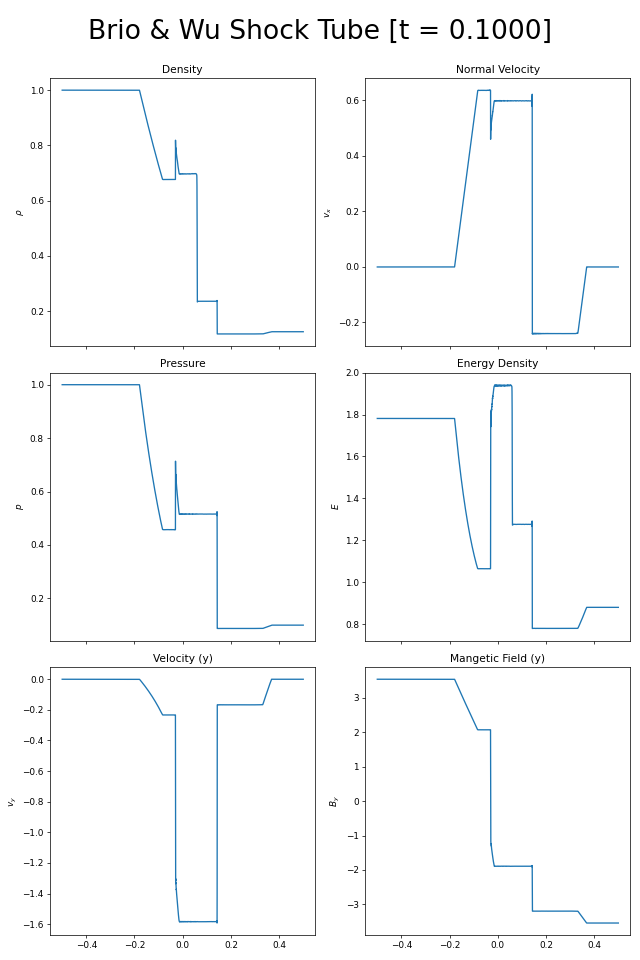
\includegraphics[width=0.5\textwidth]{../Examples/1D/Brio-Wu/Brio & Wu.png}
\caption{Reference output for the Brio \& Wu shock tube.}
\label{fig:1d-mhd-briowu}
\end{figure}

\begin{figure}[p]
\centering
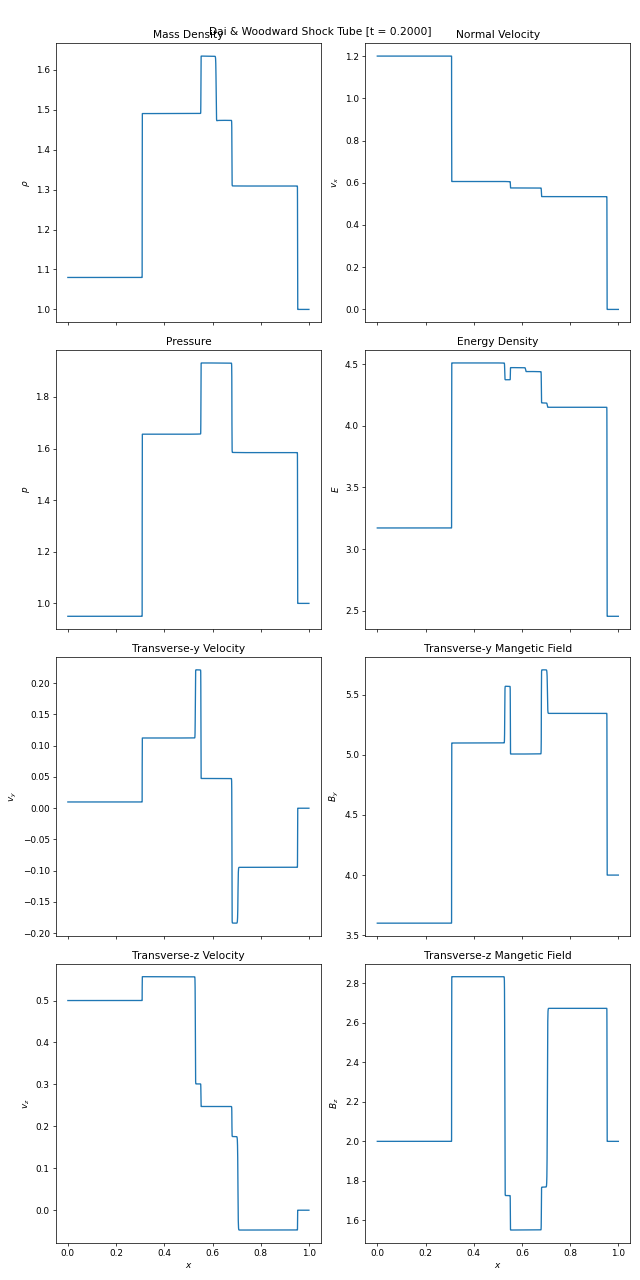
\includegraphics[width=0.7\textwidth]{../Examples/1D/Dai-Woodward/Dai & Woodward.png}
\caption{Reference output for the Dai \& Woodward shock tube.}
\label{fig:1d-mhd-daiwoodward}
\end{figure}

\begin{figure}[p]
\centering
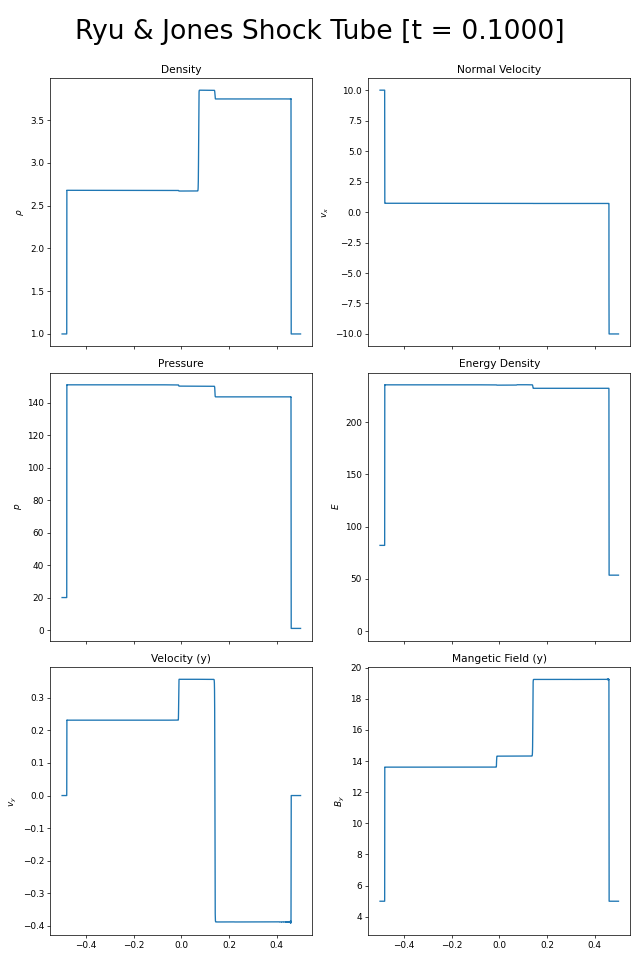
\includegraphics[width=0.7\textwidth]{../Examples/1D/Ryu-Jones/Ryu & Jones.png}
\caption{Reference output for the Ryu \& Jones shock tube.}
\label{fig:1d-mhd-ryujones}
\end{figure}

\chapter{Version History}
\textbf{Date TBD}: DRAGON v1.1 introduced the following changes
\begin{itemize}
\item Added support for user-defined passive scalars (\Cref{sec:passive}).
\begin{itemize}
\item Updated Kelvin-Helmholtz example to demonstrate passive scalars as tracers.
\item Added support for plotting any passive scalar in DRAGONGAZE
\end{itemize}
\item Added an atomic counter (\Cref{sec:atomics}) which is used to trigger a step restart if too many fallback behaviours have occurred in one advancement.
\item Added new DRAGONGAZE scripts for making bivariate plots.
\item Additional unit tests to directly verify DRAGONWING
\item Streamlined advancement and exception handling for domain-decomposed grids
\begin{itemize}
\item New \cpp{Grid::advance_step(dt)} delegates to \cpp{split_step} or \cpp{unsplit_step} as appropriate.
\item \cpp{launchParallel} now calls \cpp{grid.advance_step} instead of \cpp{grid.advance}, calls \cpp{requestRestart()} directly if an exception is thrown.
\item Removed: \cpp{Grid::on_step_fail}, \cpp{MULTITHREAD_UNAVAILABLE}
\end{itemize}
\end{itemize} 
\textbf{26 August 2026}:  Initial release of DRAGON v1.0

% ================= Bibliography =================
\bibliographystyle{plainnat}
\bibliography{references}

\end{document}
